\chapter{DESENVOLVIMENTO E RESULTADOS}\label{cap:desenvolvimento}

Este capítulo apresenta a implementação do sistema de comunicação digital proposto, detalhando cada etapa do processo, desde a geração dos bits até a recuperação do datagrama no receptor. A seguir, são descritas as principais componentes do sistema, incluindo a cadeia de transmissão, o canal de comunicação com ruído adicionado, a detecção de portadora e a cadeia de recepção.

\section{CADEIA DE TRANSMISSÃO}\label{sec:transmissao}

A primeira etapa do sistema é a geração da sequência de bits que compõem o datagrama ARGOS-3, conforme descrito na Seção \ref{sec:datagrama}. Essa sequência é multiplexada com um preâmbulo para permitir a sincronização de símbolos no receptor. Em seguida, os bits são codificados utilizando codificação de linha para melhorar as características espectrais do sinal modulado, como detalhado na Seção \ref{sec:line_coding}.

\subsection{Sequência de transmissão}\label{sec:geracao_bits}

O primeiro passo na cadeia de transmissão é a geração da sequência de bits que compõem o datagrama \gls{ARGOS-III}, conforme ilustrado na \autoref{fig:datagrama_time}, para a montagem do datagrama é necessário o número de identificação da PCD, \gls{ipcd}, e os dados que serão transmitidos (payload), conforme detalhado na seção \ref{sec:datagrama}, desta forma, o comprimento da mensagem \gls{Tm}, o campo de identificação da PCD \gls{pcdid} e a cauda do datagrama \gls{Em} podem ser calculados. 

\begin{figure}[H]
	\centering
	\caption{Streambits do datagrama ARGOS-3}\label{fig:datagrama_time}
	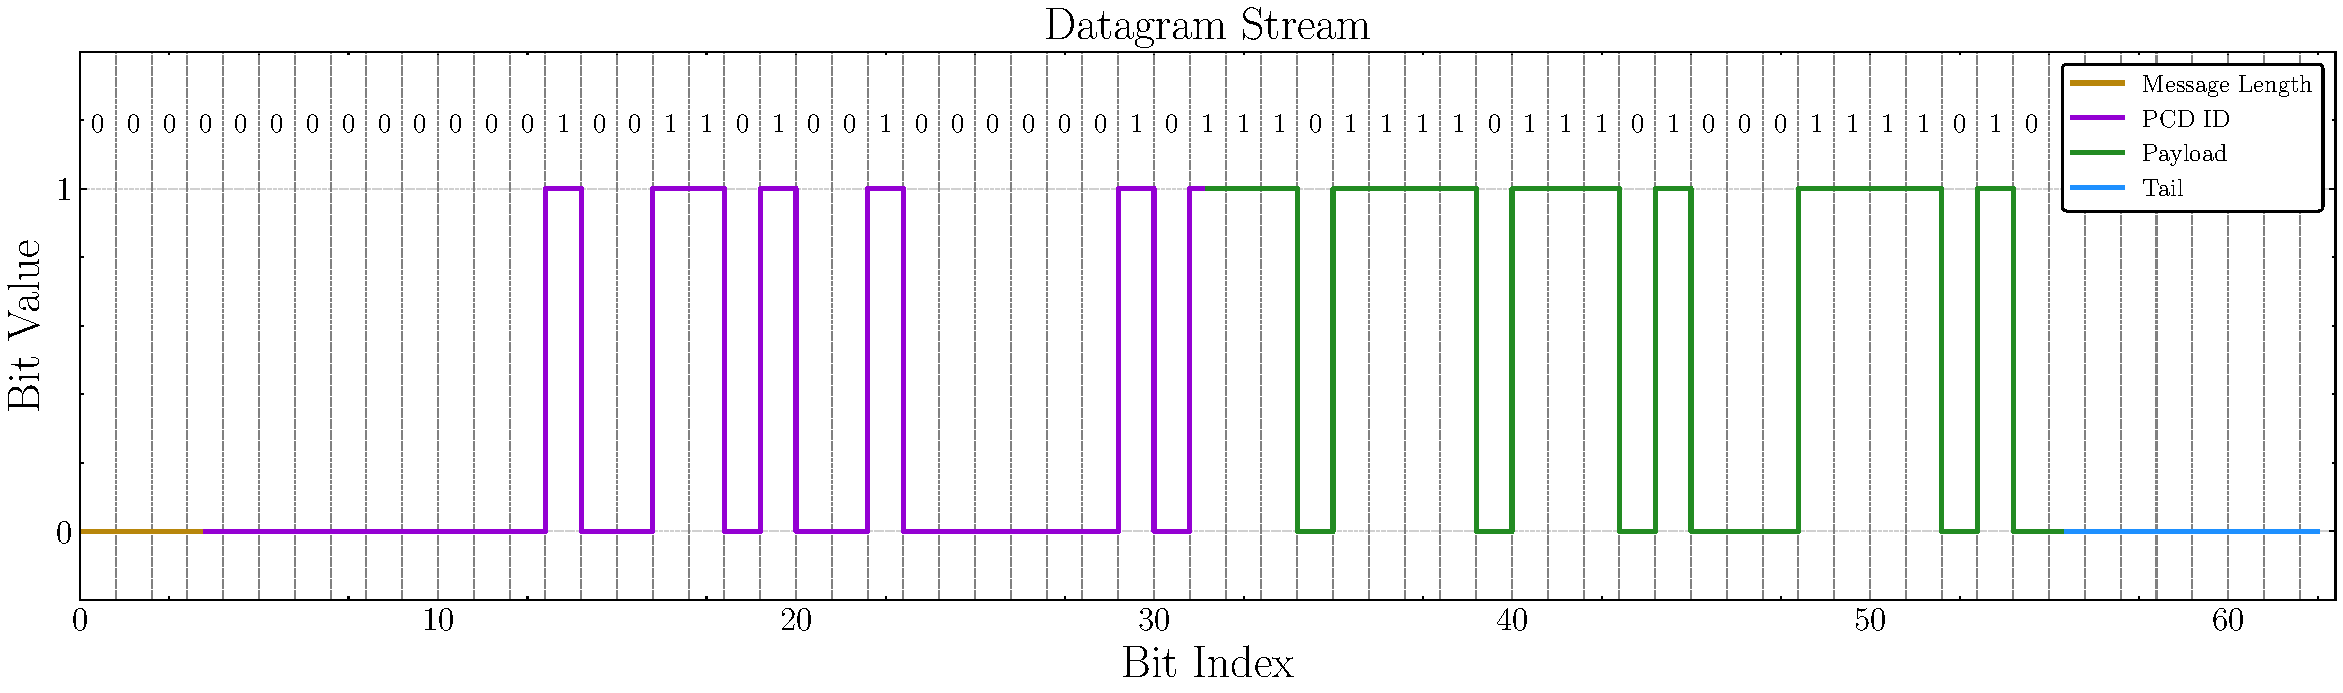
\includegraphics[width=\linewidth]{assets/cap3/transmitter_datagram_time.pdf}
\end{figure}

Após a montagem dos bits \gls{ut} do datagrama, os mesmos são codificados utilizando codificação convolucional, conforme detalhado na seção \ref{sec:conv_coding}, resultando nos vetores de bits \gls{vt0} e \gls{vt1}, que por sua vez são embaralhados resultando nas sequências \gls{Xn} e \gls{Yn} para os canais \gls{cI} e \gls{cQ}, respectivamente, o processo de codificação convolucional aplicado no vetor \gls{ut} é ilustrado na \autoref{fig:transmitter_conv_time}.

\begin{figure}[H]
	\centering
	\caption{Codificação convolucional do datagrama ARGOS-3}\label{fig:transmitter_conv_time}
	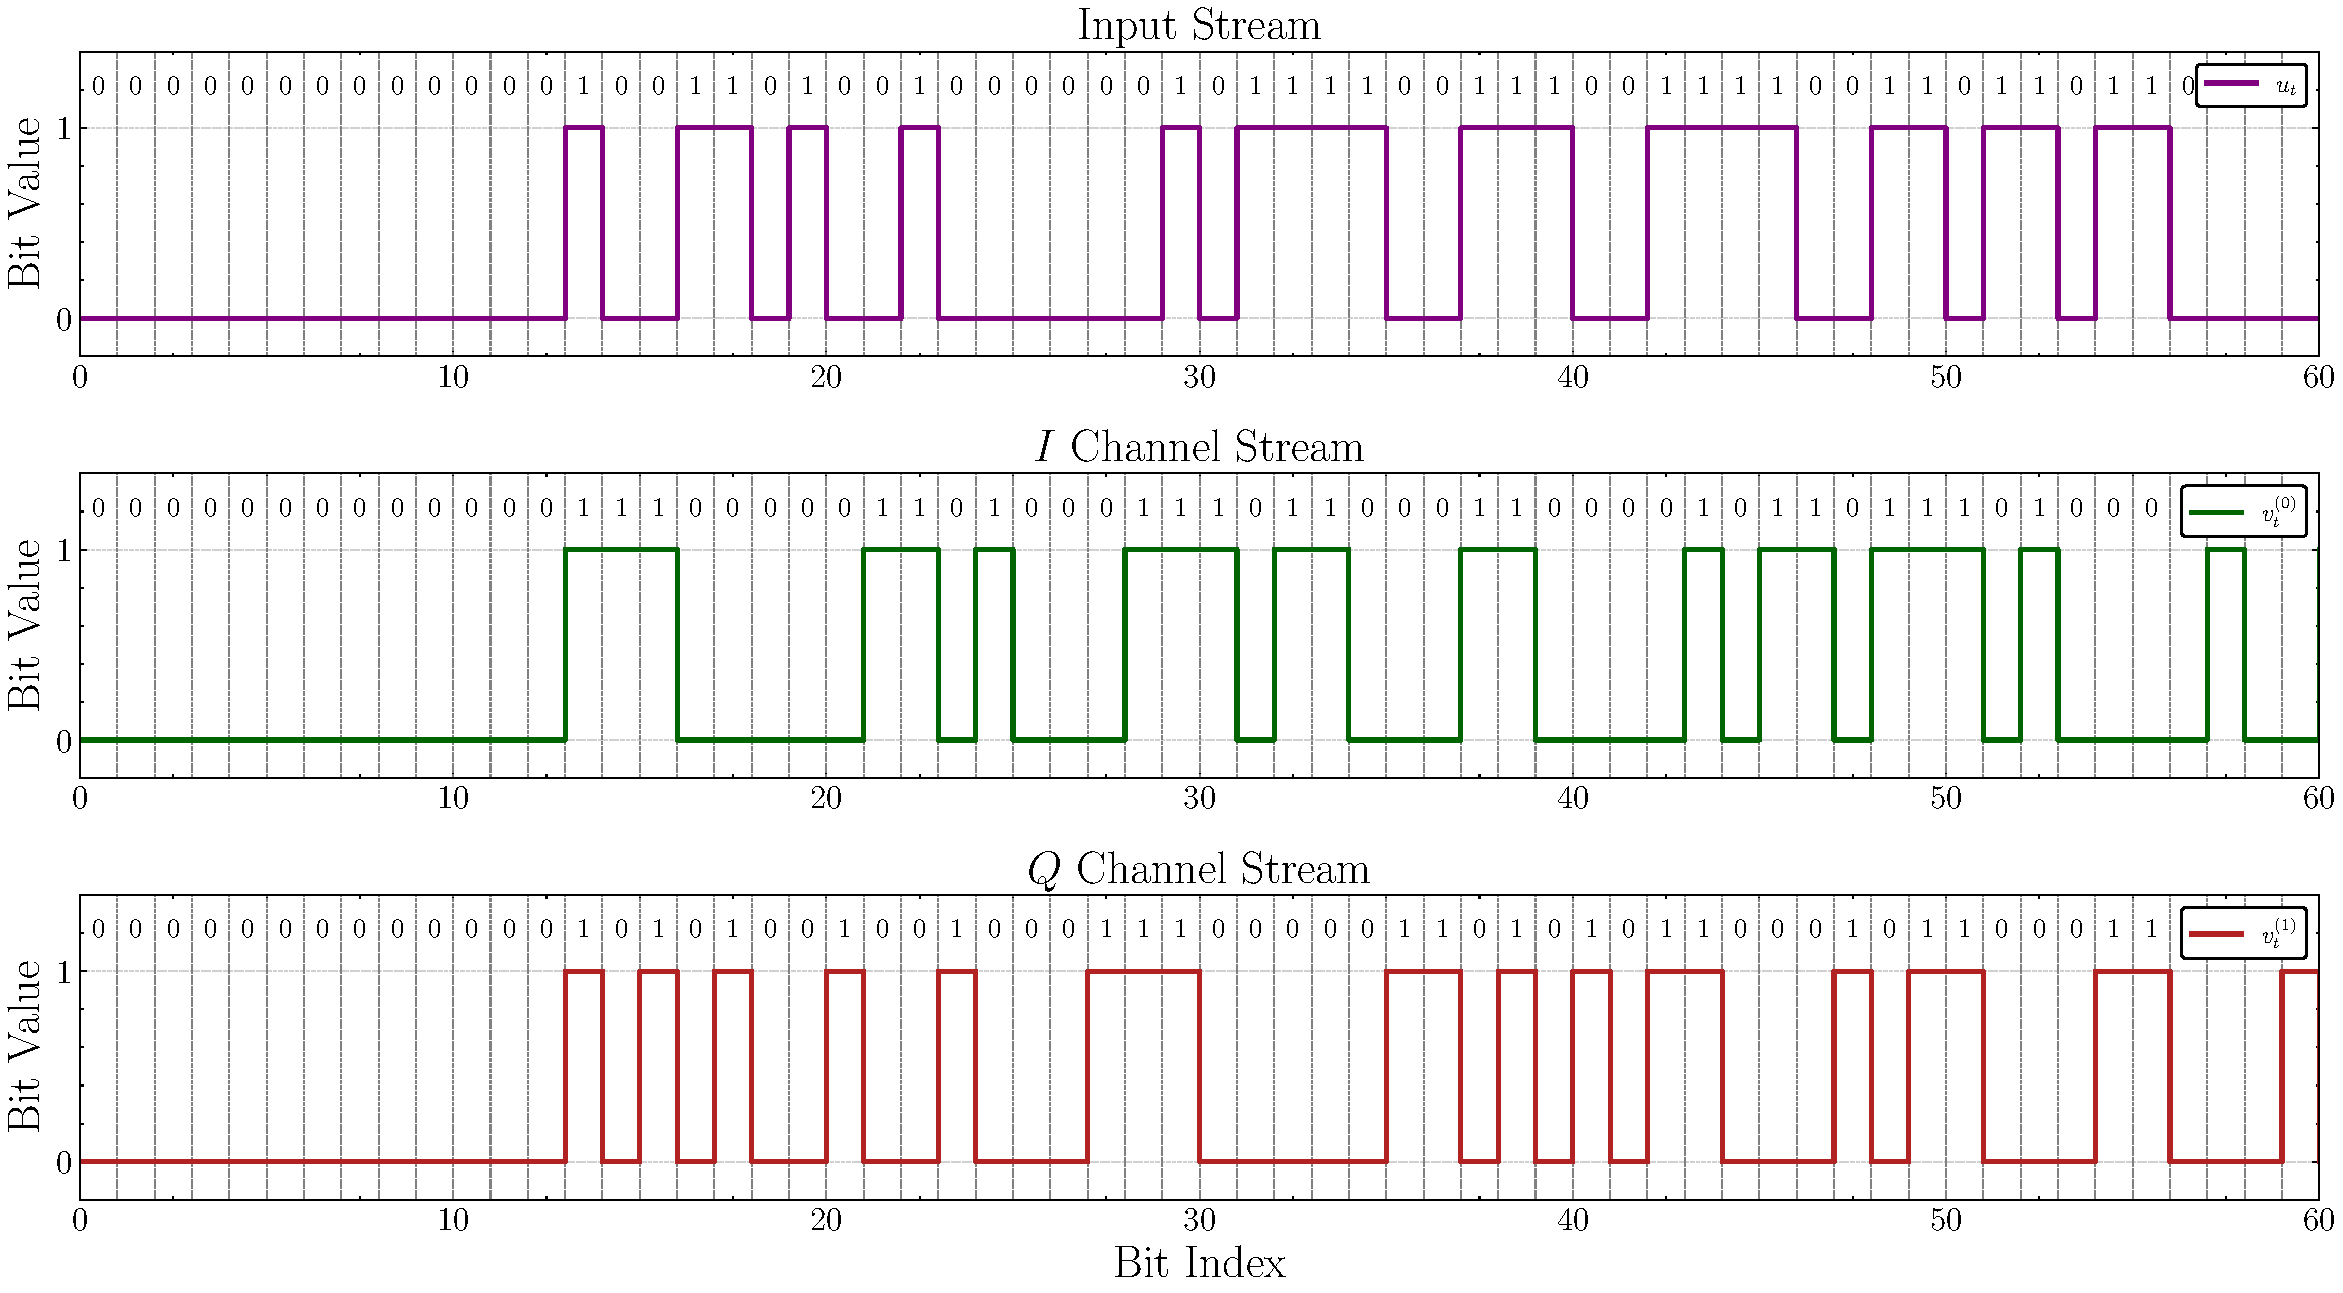
\includegraphics[width=\linewidth]{assets/cap3/transmitter_conv_time.pdf}
\end{figure}

As sequências \gls{Xn} e \gls{Yn} já embaralhadas, são então multiplexadas com o preâmbulo \gls{SIn} e \gls{SQn} dos canais \gls{cI} e \gls{cQ} respectivamente, gerados conforme apresentado na seção \ref{sec:preambulo}. A adição das sequências é fundamental para permitir a sincronização de símbolos no receptor, esse processo é ilustrado na \autoref{fig:mux_time}.

\begin{figure}[H]
	\centering
	\caption{Multiplexação com preâmbulo}\label{fig:mux_time}
	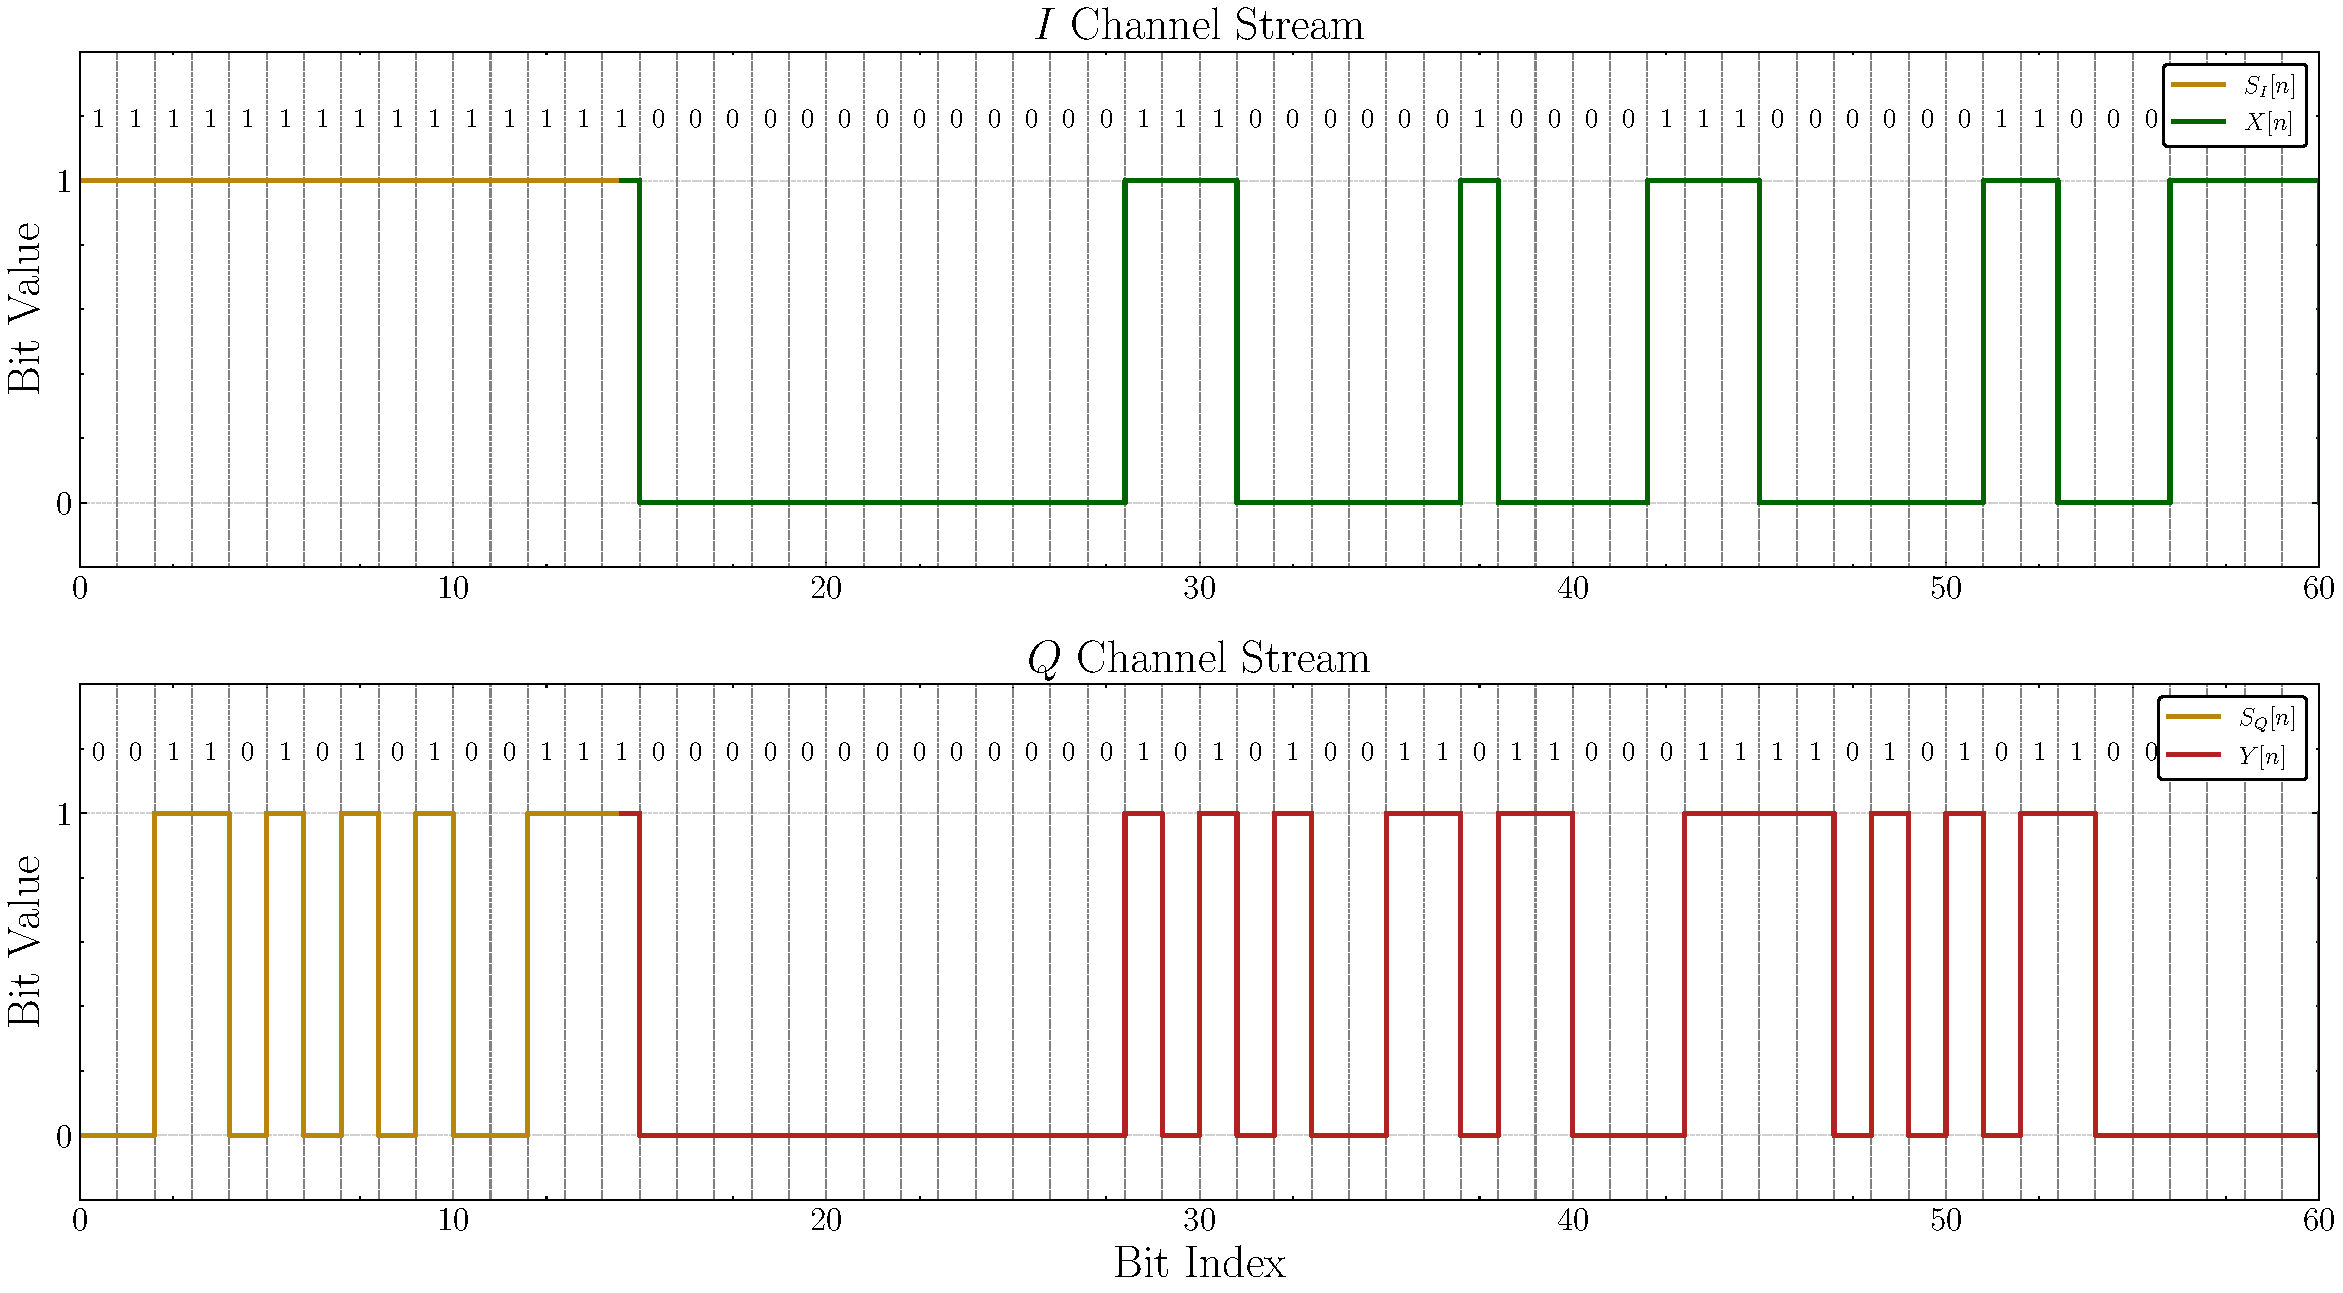
\includegraphics[width=\linewidth]{assets/cap3/transmitter_mux_time.pdf}
\end{figure}

Em seguida, os bits são codificados utilizando codificação de linha para melhorar as características espectrais do sinal modulado, como detalhado na seção \ref{sec:line_coding}, neste processo é utilizado apenas codificação \gls{NRZ} para os dois canais, pois a técnica \gls{Manchester} será aplicada posteriormente na modulação de pulso do canal \gls{cQ}, o processo de codificação de linha de ambos os canais é ilustrado na \autoref{fig:encoder_time}.

\begin{figure}[H]
	\centering
	\caption{Codificação de linha}\label{fig:encoder_time}
	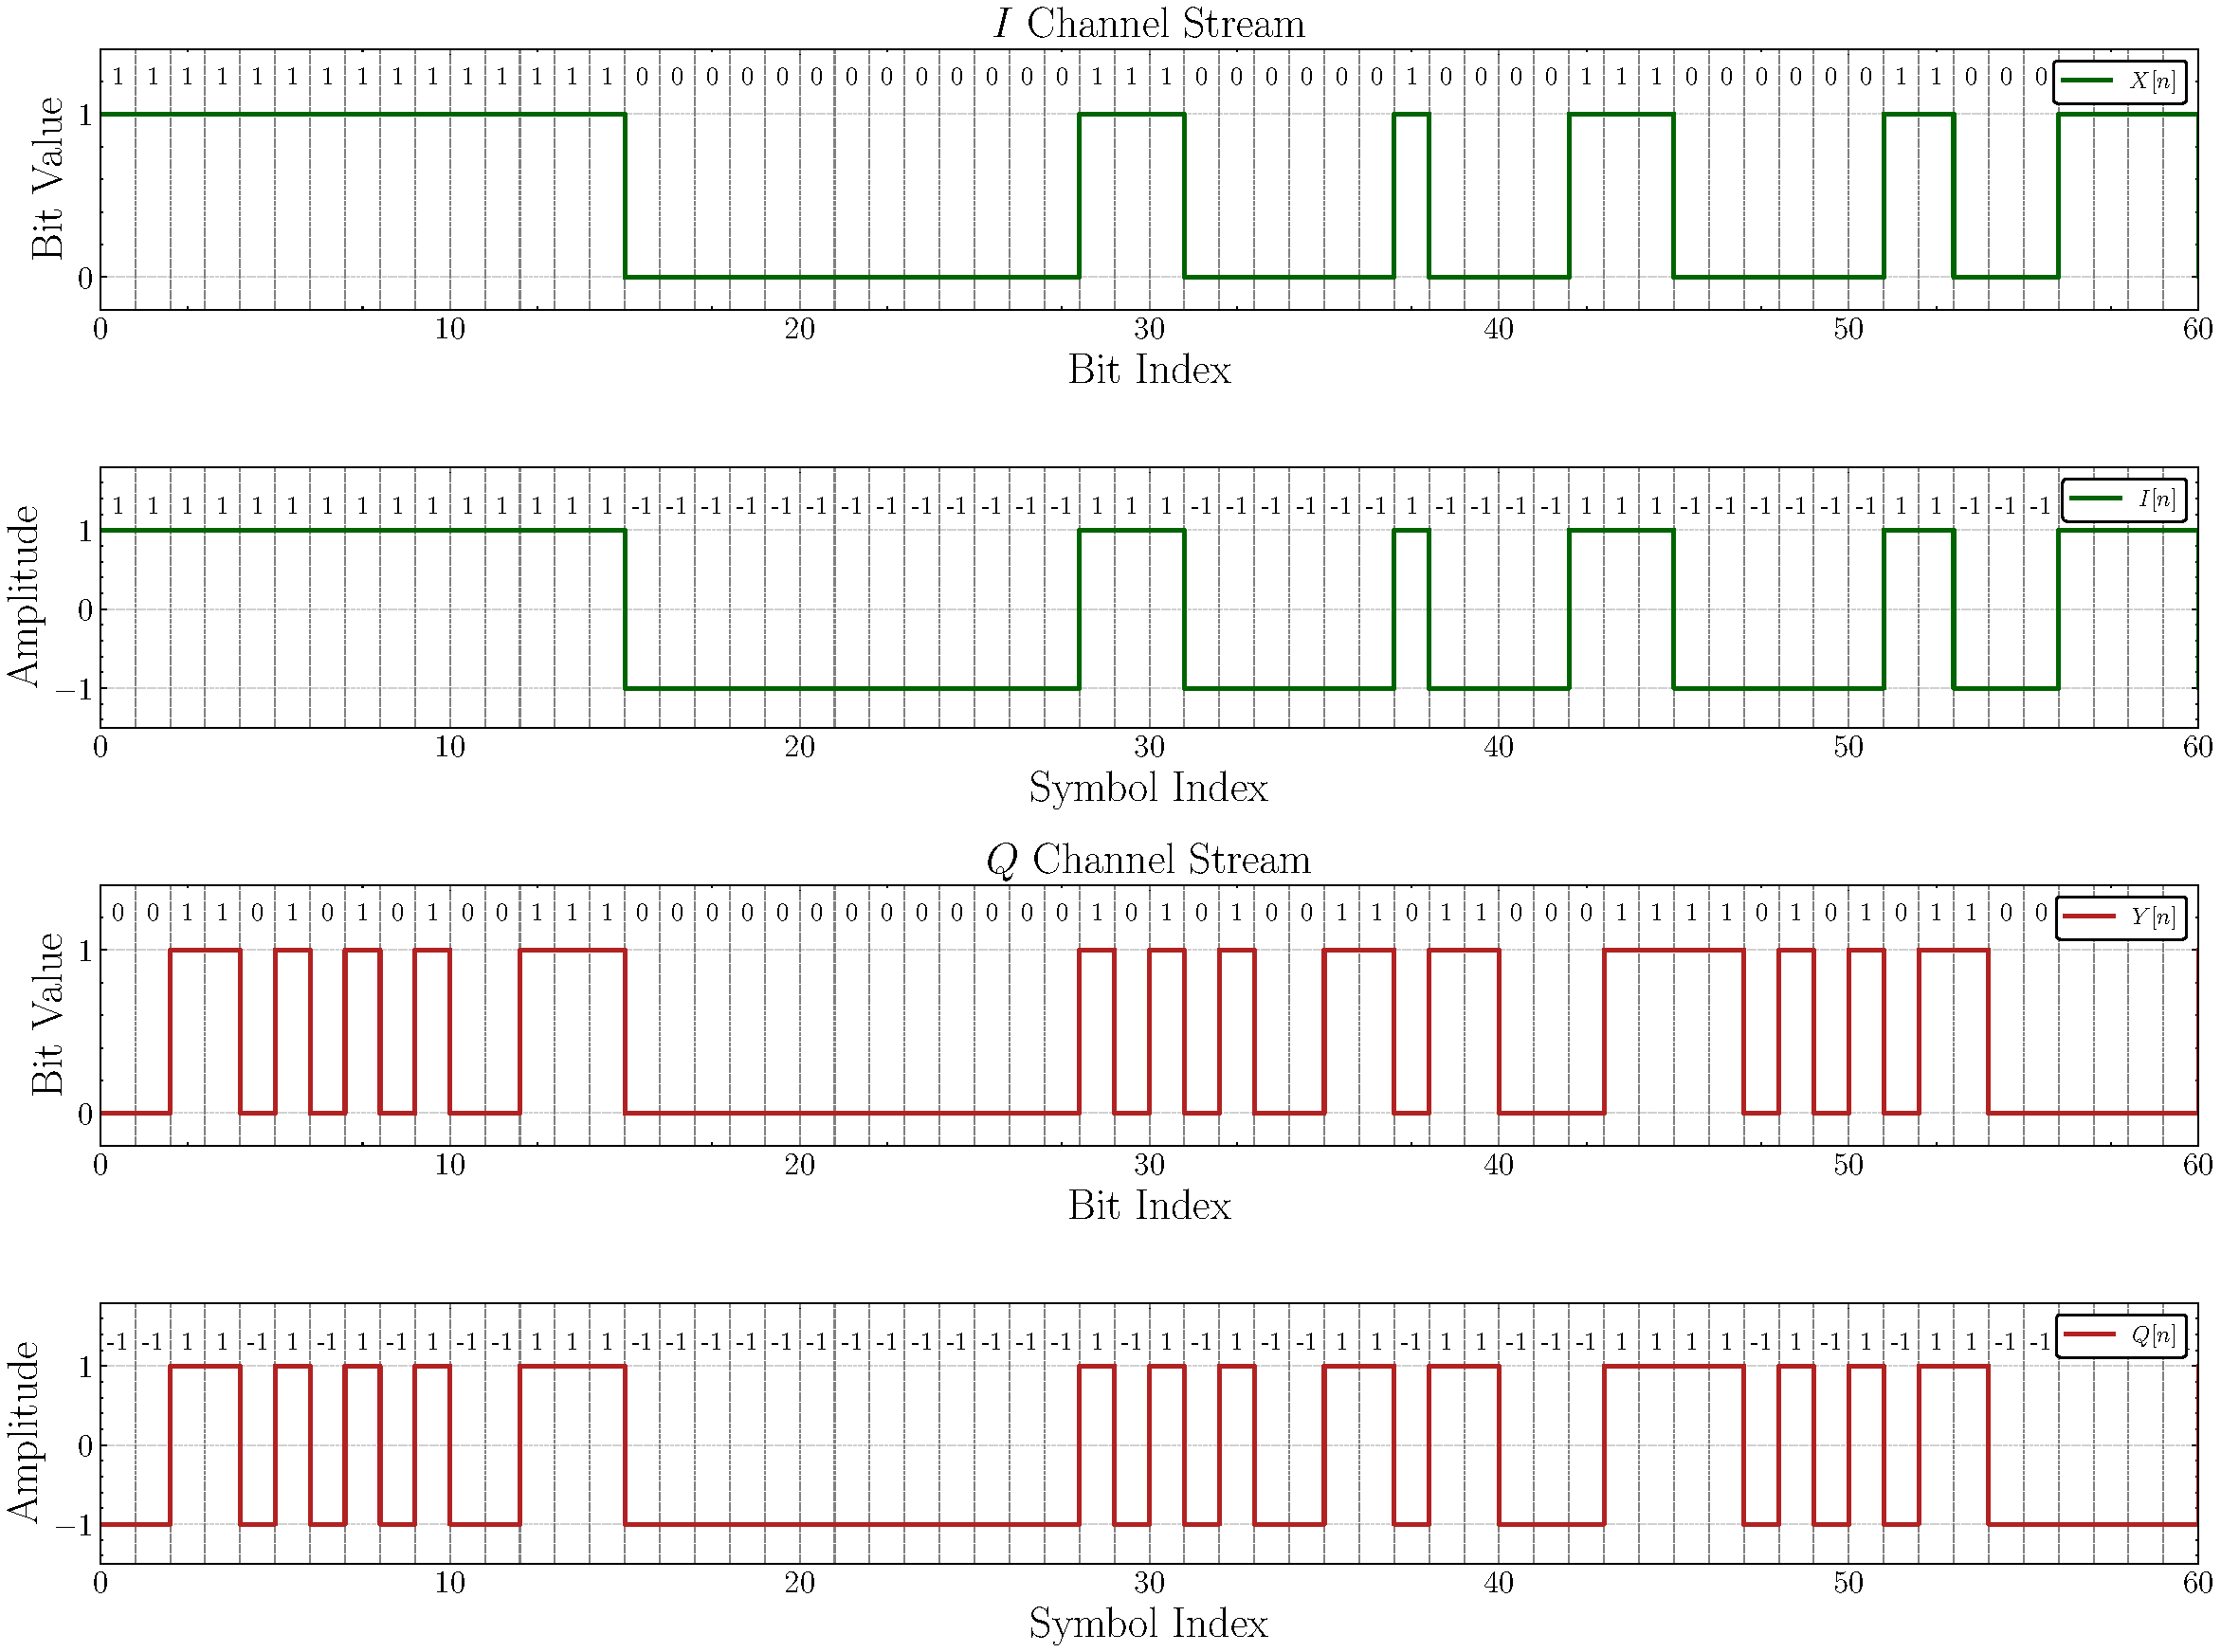
\includegraphics[width=\linewidth]{assets/cap3/transmitter_encoder_time.pdf}
\end{figure}

As sequências de símbolos \gls{In} e \gls{Qn} resultantes da codificação de linha, estão prontas para serem moduladas utilizando modulação de pulso. 

\subsection{Modulação de pulso RRC e Manchester}

Após a montagem das sequências de símbolos \gls{In} e \gls{Qn}, o próximo passo é a modulação de pulso, onde o canal \gls{cI} utiliza um filtro de pulso \gls{RRC} e o canal \gls{cQ} utiliza um filtro de pulso \gls{Manchester}, conforme detalhado na seção \ref{sec:line_coding}. A modulação de pulso é fundamental para reduzir a largura de banda \gls{W} do sinal que está sendo transmitido e também reduzir a interferência entre símbolos \gls{ISI}. O processo de modulação de pulso dos canais \gls{cI} e \gls{cQ} é ilustrado na \autoref{fig:pulse_modulate_diagram}.

\begin{figure}[H]
    \centering
    \caption{Diagrama de blocos do modulador de pulso para os canais $I$ e $Q$}\label{fig:pulse_modulate_diagram}
    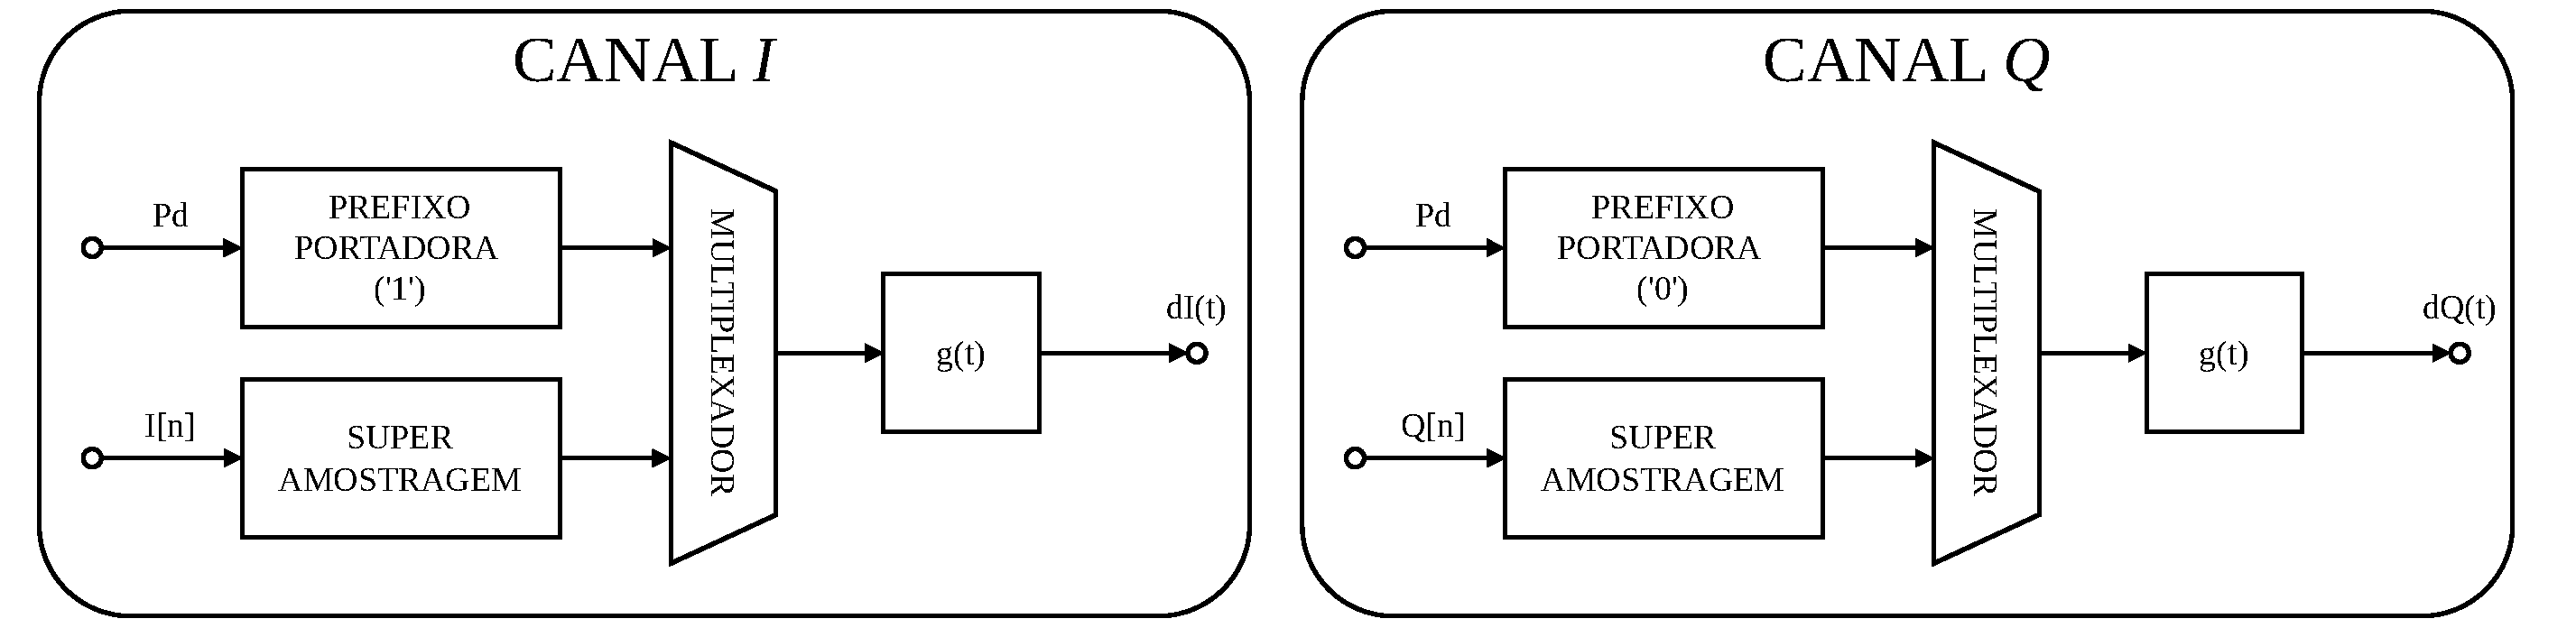
\includegraphics[width=\linewidth]{assets/diagrams/pulse_modulate.pdf}
\end{figure}

\subsubsection{Pulso RRC e Manchester}

Antes de aplicar a modulação de pulso, é necessário gerar os filtros de pulso \gls{RRC} e \gls{Manchester}, que serão utilizados para modular os canais \gls{cI} e \gls{cQ}, respectivamente. A resposta ao impulso do filtro \gls{RRC} é ilustrada na \autoref{fig:impulse_response_rrc}, e é calculada conforme apresentado na seção \ref{sec:pulse_modulation}. 

\begin{figure}[H]
	\centering
	\caption{Resposta ao impulso - Pulso RRC}\label{fig:impulse_response_rrc}
	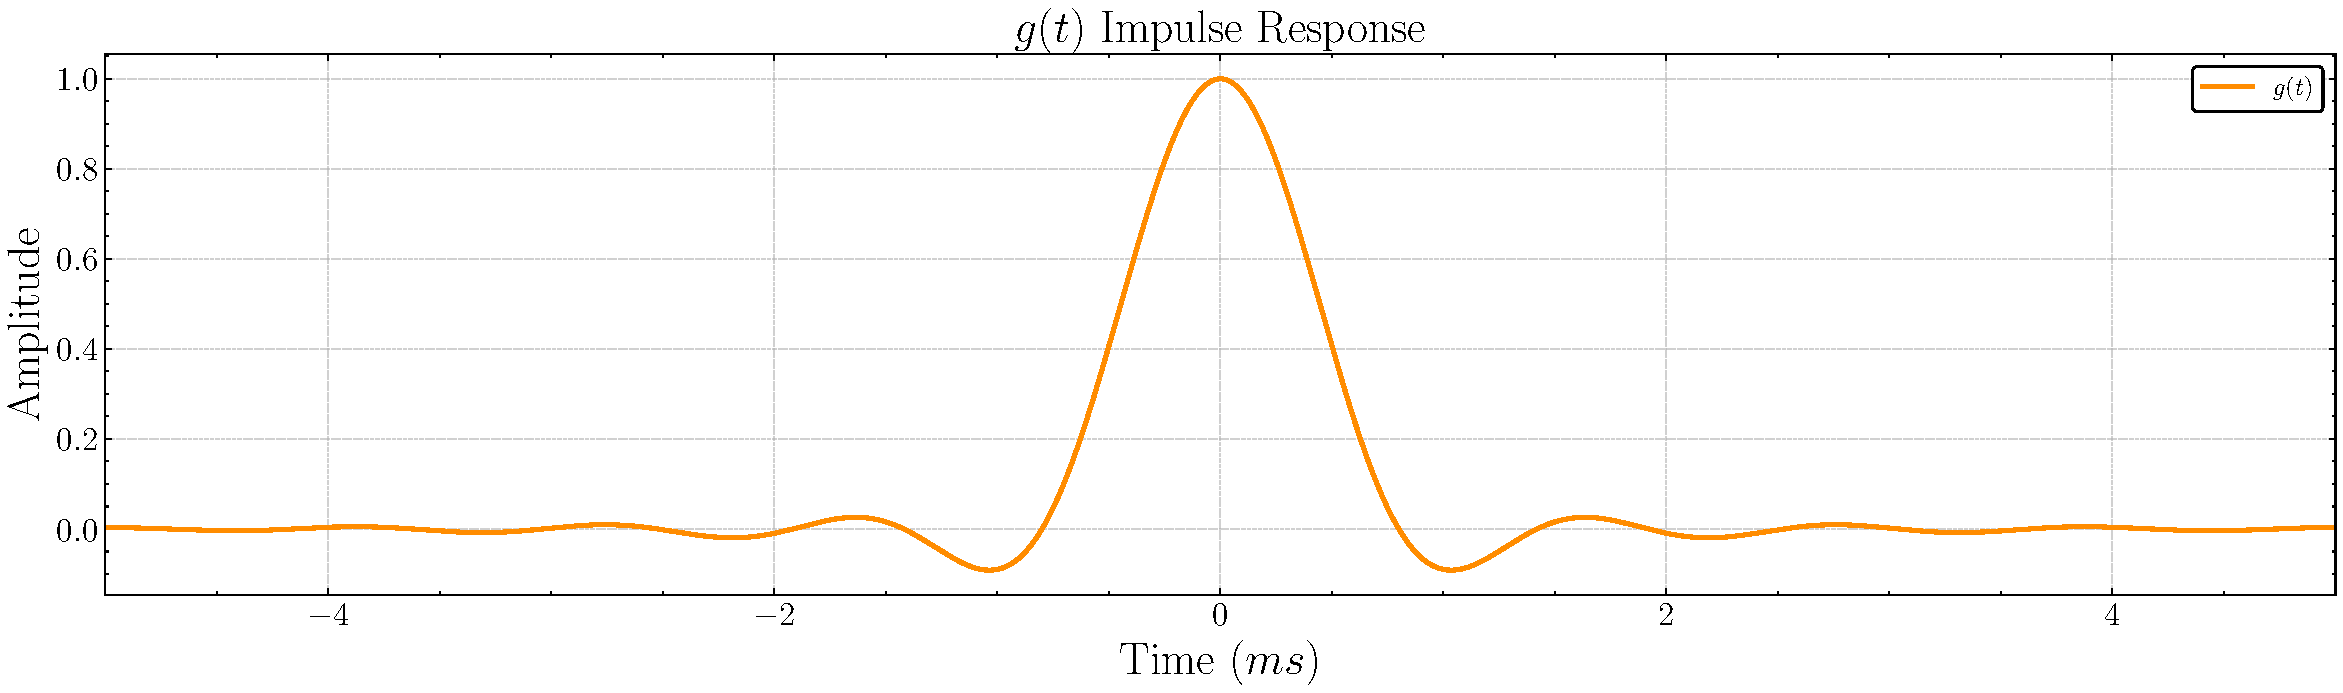
\includegraphics[width=\linewidth]{assets/cap3/example_formatter_impulse.pdf}
\end{figure}

Já o pulso \gls{Manchester} é gerado através de uma soma de dois pulsos \gls{RRC} deslocados no tempo, um positivo deslocado em $T_b/2$ e outro negativo deslocado em $-T_b/2$, conforme ilustrado na \autoref{fig:impulse_response_man}. O calculo do pulso pode ser expresso como 

\begin{equation}
g_{MAN}(t) = g_{RRC}(t + T_b/2) - g_{RRC}(t - T_b/2)
\end{equation}

Onde $g_{MAN}(t)$ é o pulso Manchester, $g_{RRC}(t)$ é o pulso RRC e $T_b$ é o tempo de bit. A resposta ao impulso do filtro \gls{Manchester} é ilustrada na \autoref{fig:impulse_response_man}.

\begin{figure}[H]
	\centering
	\caption{Resposta ao impulso - Pulso Manchester}\label{fig:impulse_response_man}
	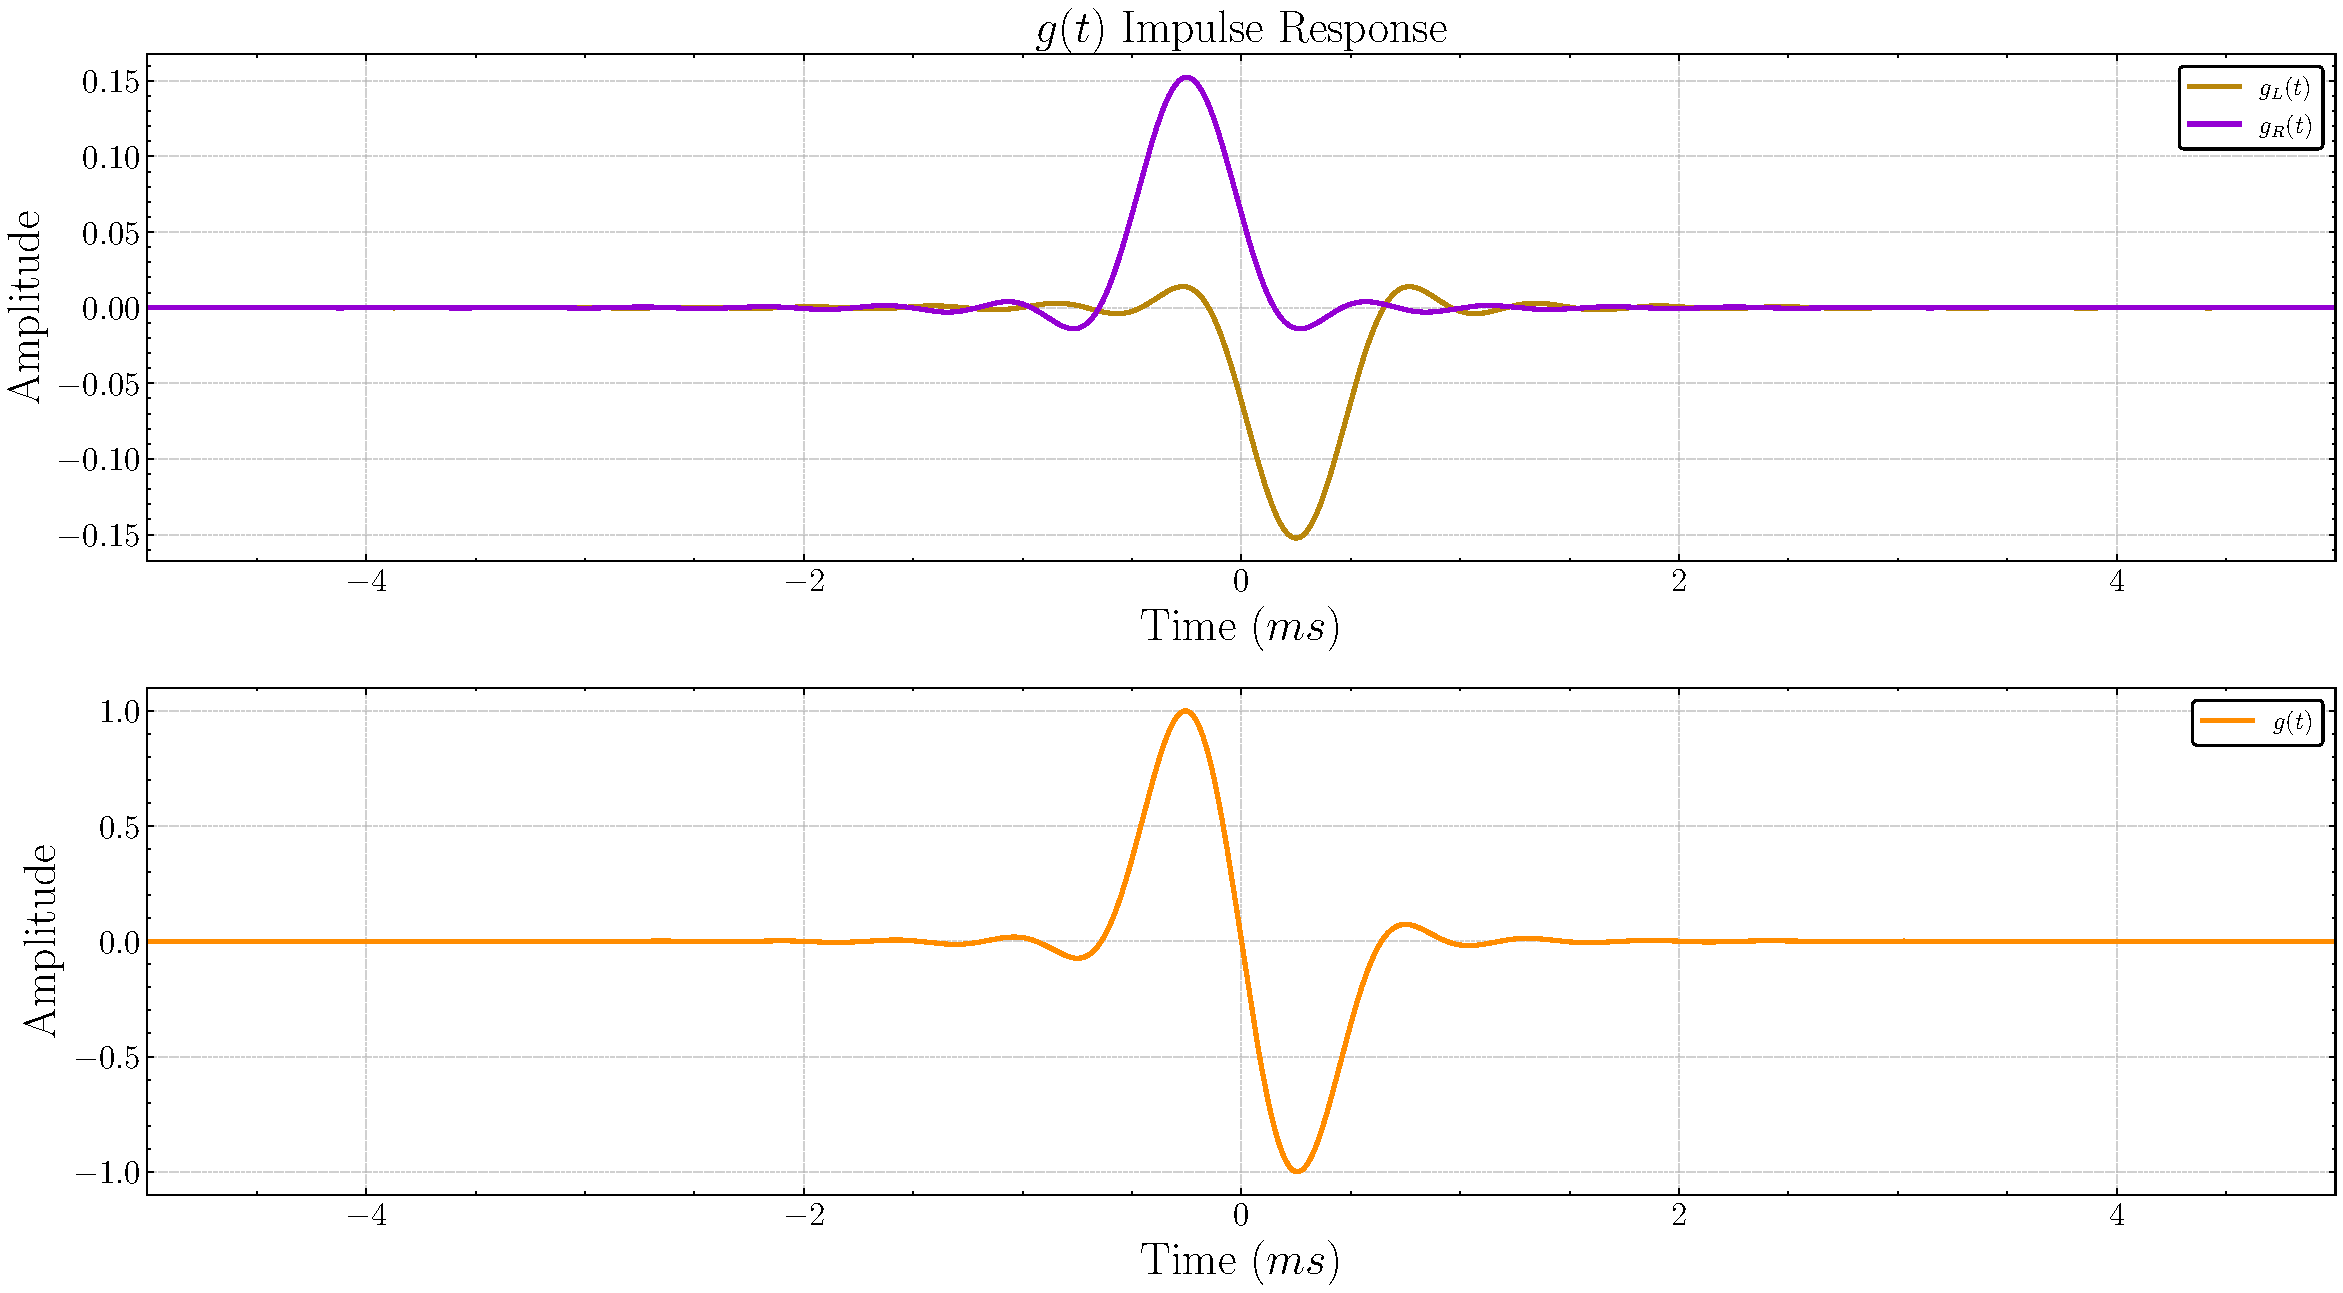
\includegraphics[width=\linewidth]{assets/cap3/example_formatter_impulse_man.pdf}
\end{figure}

A utilização do pulso \gls{Manchester} no canal \gls{cQ} ao invés da codificação de linha \gls{Manchester} proposta originalmente tem como objetivo simplificar a implementação do sistema, reduzindo a complexidade computacional e o número de etapas necessárias na cadeia de transmissão. 

\subsubsection{Modulação de pulso dos canais I e Q}

Uma vez com os filtros de pulso \gls{RRC} e \gls{Manchester} gerados, é possível aplicar a modulação de pulso nos canais \gls{cI} e \gls{cQ}, respectivamente gerando os sinais \gls{dI} e \gls{dQ} modulados em banda base. Esse processo envolve a superamostragem dos vetores de símbolos \gls{In} e \gls{Qn}, em função da frequência de amostragem \gls{fs}, seguida da filtragem com os respectivos filtros de pulso. 

O resultado são as sequências \gls{dI} e \gls{dQ} contínuas ao longo do tempo \gls{t}, onde cada bit de informação é transmitido durante um período de tempo $\text{ \gls{Tb}} = 1/ \text{\gls{Rb}}$ (tempo de bit), definido com base na taxa de bit \gls{Rb}. A modulação de pulso dos canais \gls{cI} e \gls{cQ} é ilustrada na \autoref{fig:transmitter_formatter_time}.

\begin{figure}[H]
	\centering
	\caption{Modulação de pulso dos canais $I$ e $Q$}\label{fig:transmitter_formatter_time}
	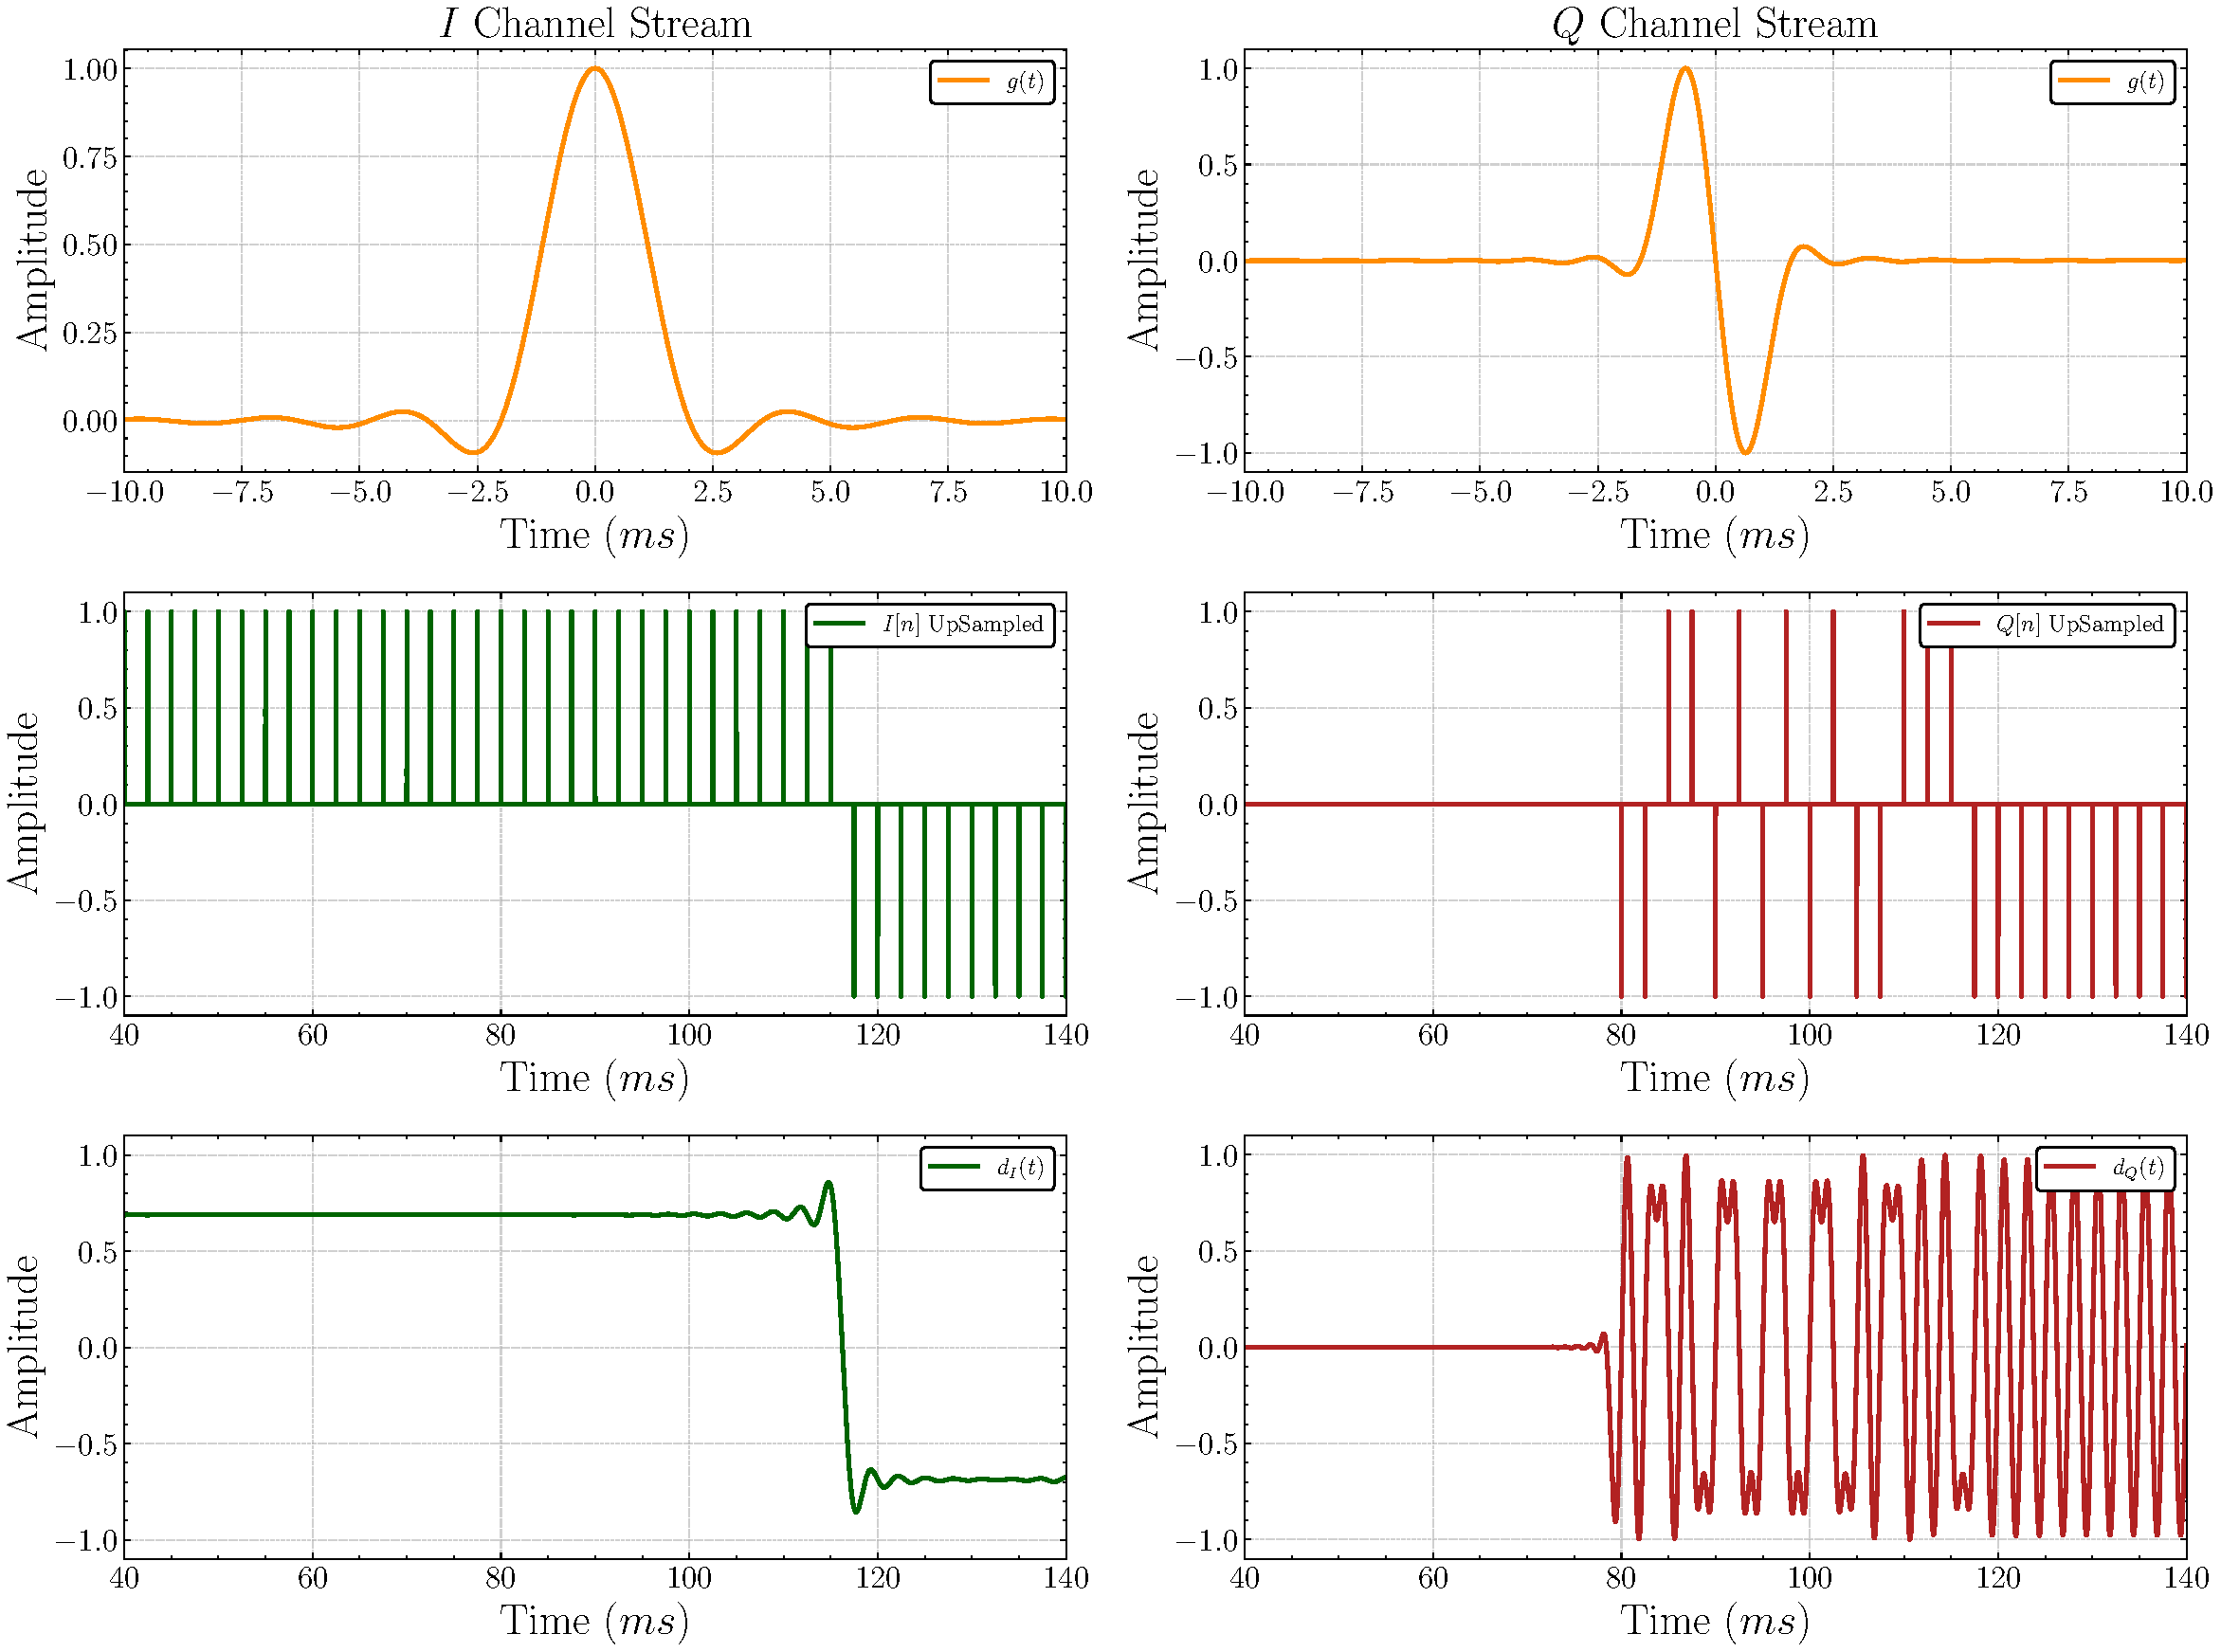
\includegraphics[width=\linewidth]{assets/cap3/transmitter_formatter_time_comp.pdf}
\end{figure}

As sequências \gls{dI} e \gls{dQ} estão agora prontas para serem moduladas em banda passante utilizando modulação em fase em quadratura (\gls{QPSK}), conforme detalhado na seção \ref{sec:qpsk}.

\subsection{Modulação em fase em quadratura (QPSK)}\label{sec:qpsk}

Na modulação \gls{QPSK}, os sinais modulados em banda base \gls{dI} e \gls{dQ} são utilizados para modular uma componente senoideal e uma componente cossenoidal, respectivamente, com frequência \gls{fc}, o somatório dessas duas componentes moduladas resulta no sinal modulado em banda passante \gls{st}, conforme ilustrado na \autoref{fig:transmitter_modulator_time}.

\begin{figure}[H]
	\centering
	\caption{Modulação em banda passante canais $I$ e $Q$}\label{fig:transmitter_modulator_time}
	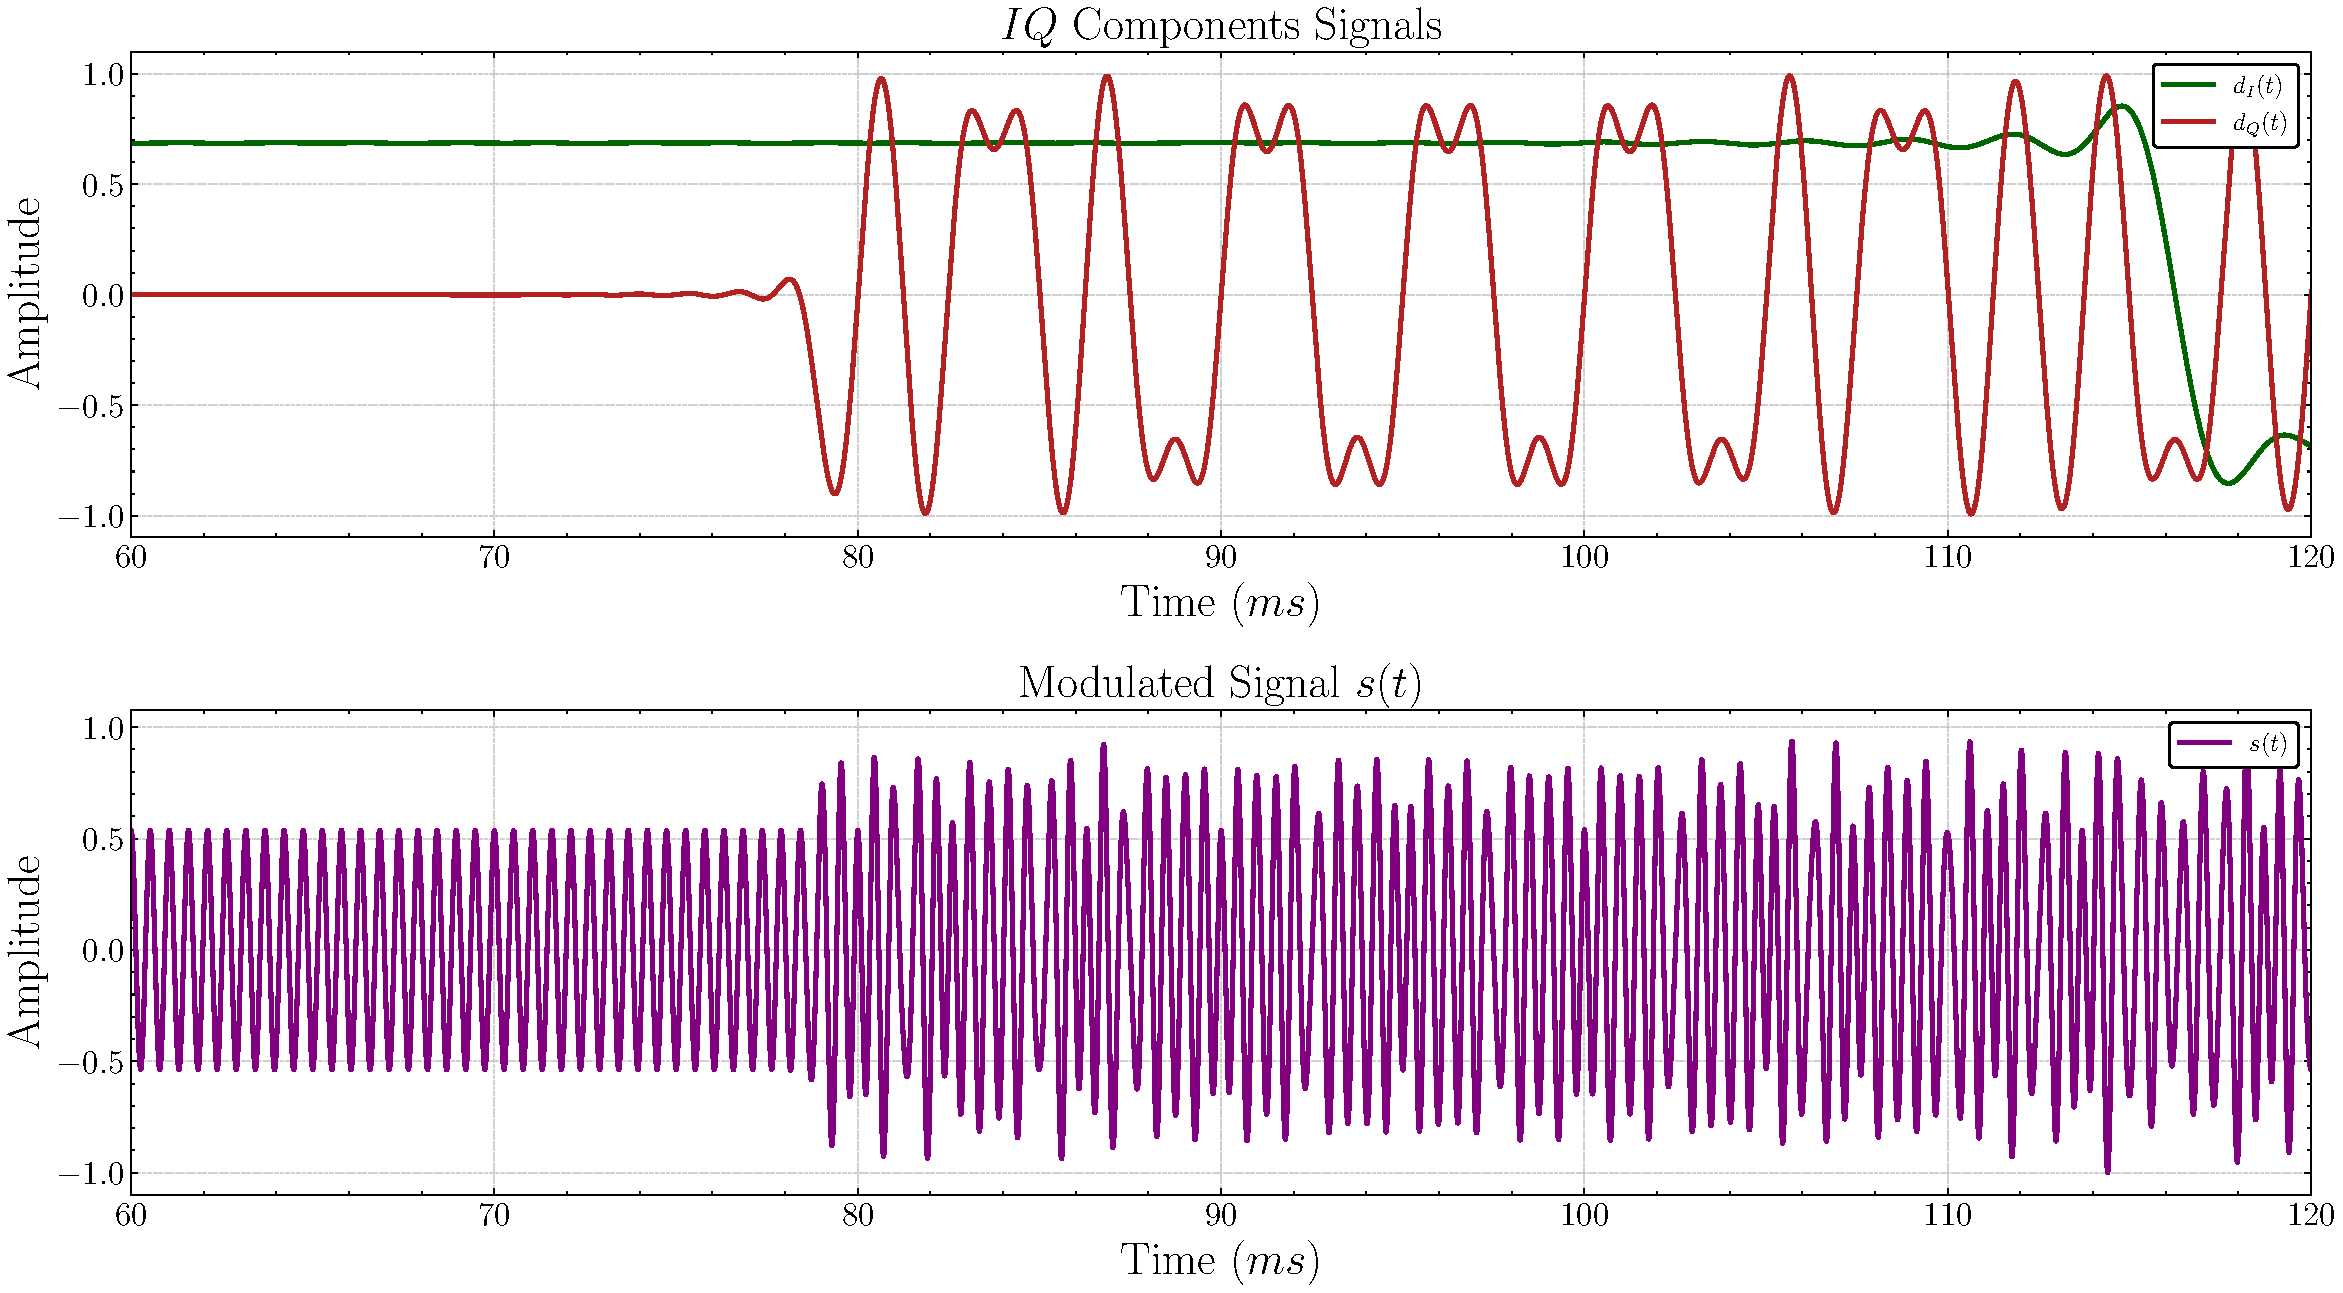
\includegraphics[width=\linewidth]{assets/cap3/transmitter_modulator_time.pdf}
\end{figure}

A partir do sinal modulado \gls{st}, é possível observar a constelação do sinal \gls{QPSK}, isto é o comportamento do sinal \gls{st} no \gls{iqplane}, que idealmente para o \gls{QPSK} é composto por quatro pontos distintos, cada um representando uma combinação única dos bits transmitidos pelos canais \gls{cI} e \gls{cQ}. A constelação do sinal modulado \gls{st} é ilustrada na \autoref{fig:transmitter_modulator_constellation}, onde é possível observar a fase do sinal modulado e a constelação resultante no \gls{iqplane}.


\begin{figure}[H]
	\centering
	\caption{Fase e Constelação do sinal modulado $s(t)$}\label{fig:transmitter_modulator_constellation}
	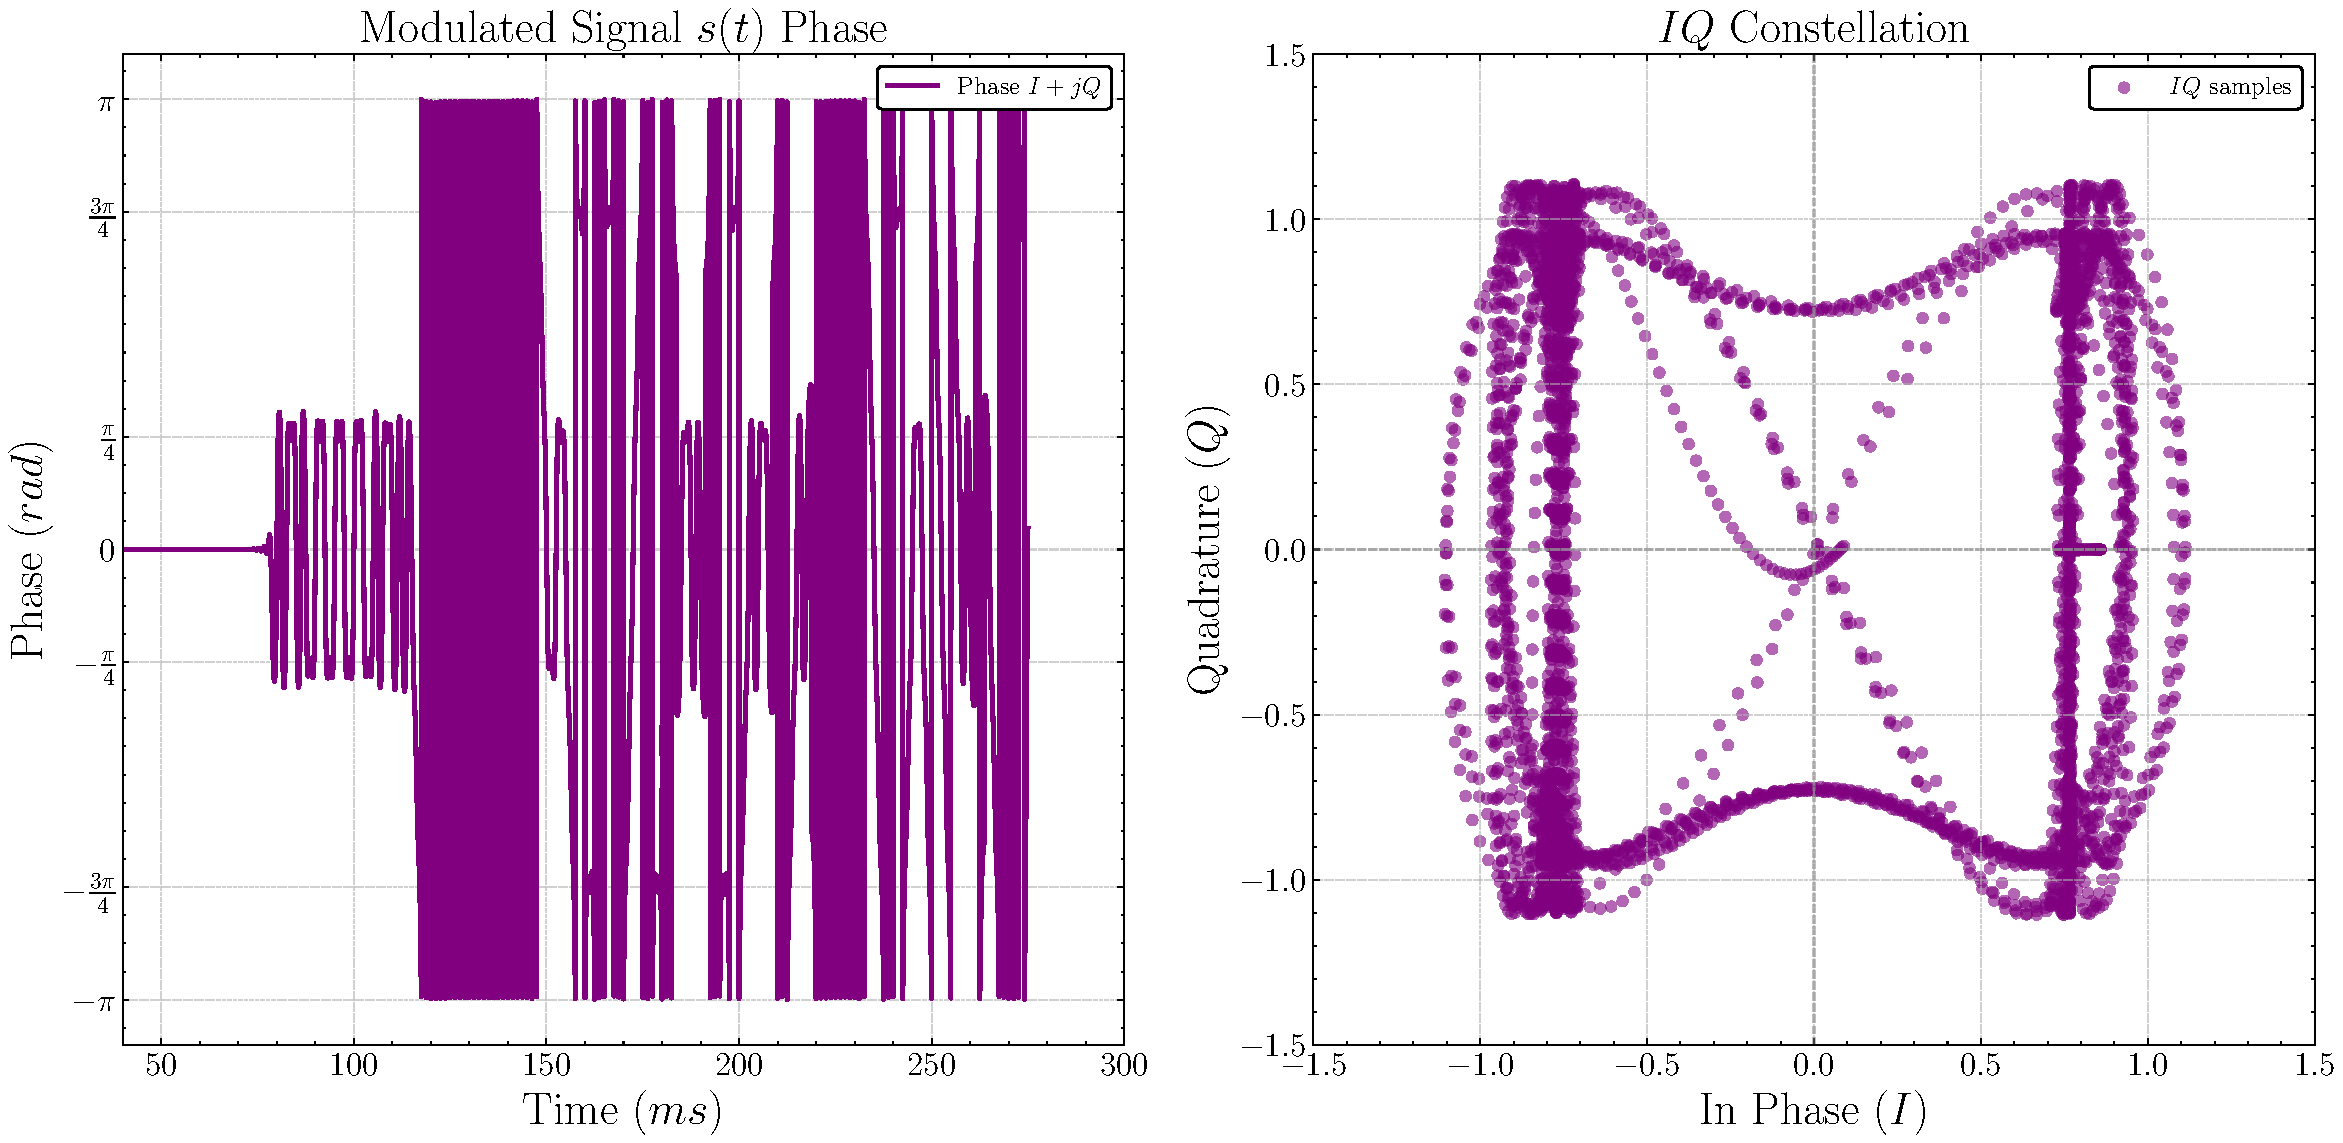
\includegraphics[width=\linewidth]{assets/cap3/transmitter_modulator_constellation.pdf}
\end{figure}


\subsubsection{Adição de portadora pura}

Ao se observar as figuras \ref{fig:transmitter_modulator_time} e \ref{fig:transmitter_formatter_time} pode-se notar que no inicio da transmissão, a componente \gls{dI} está com amplitude estável e proxima á $`1`$, enquanto que a componente \gls{dQ} está estável com amplitude igual a $`0`$, essa é configuração é proposital dentro do \gls{Pd} para que a sequência resultante modulada em banda passante tenha um periodo de fase estável, ou seja, uma portadora pura, antes do inicio da transmissão dos dados. O equacionamento para o período de portadora pura pode ser expresso como

\begin{equation}
    s(t) = 1(t) \cdot \cos(2\pi f_c t) - 0(t) \cdot \sin(2\pi f_c t) \mapsto s(t) = \cos(2\pi f_c t)
\end{equation}

\noindent Onde $1(t)$ é a componente \gls{dI} com valor constante $`1`$ e $0(t)$ é a componente \gls{dQ} com valor constante $`0`$. O período de portadora pura é fundamental para o receptor identificar a frequência da portadora \gls{fc} e realizar a detecção do sinal corretamente, conforme detalhado na seção \ref{sec:detector}. A duração do período de portadora pura é definida pelo parâmetro \gls{Pd}, que no padrão \gls{ARGOS-III} é aproximadamente $0.082$ segundos.

Com o sinal modulado em banda passante \gls{st} conforme definido acima, podemos também verificar a presença da portadora pura nos primeiros instantes da transmissão, isto é ilustrado na figura \ref{fig:transmitter_modulator_portadora}.

\begin{figure}[H]
	\centering
	\caption{Comparação de portadora pura e sinal modulado}\label{fig:transmitter_modulator_portadora}
	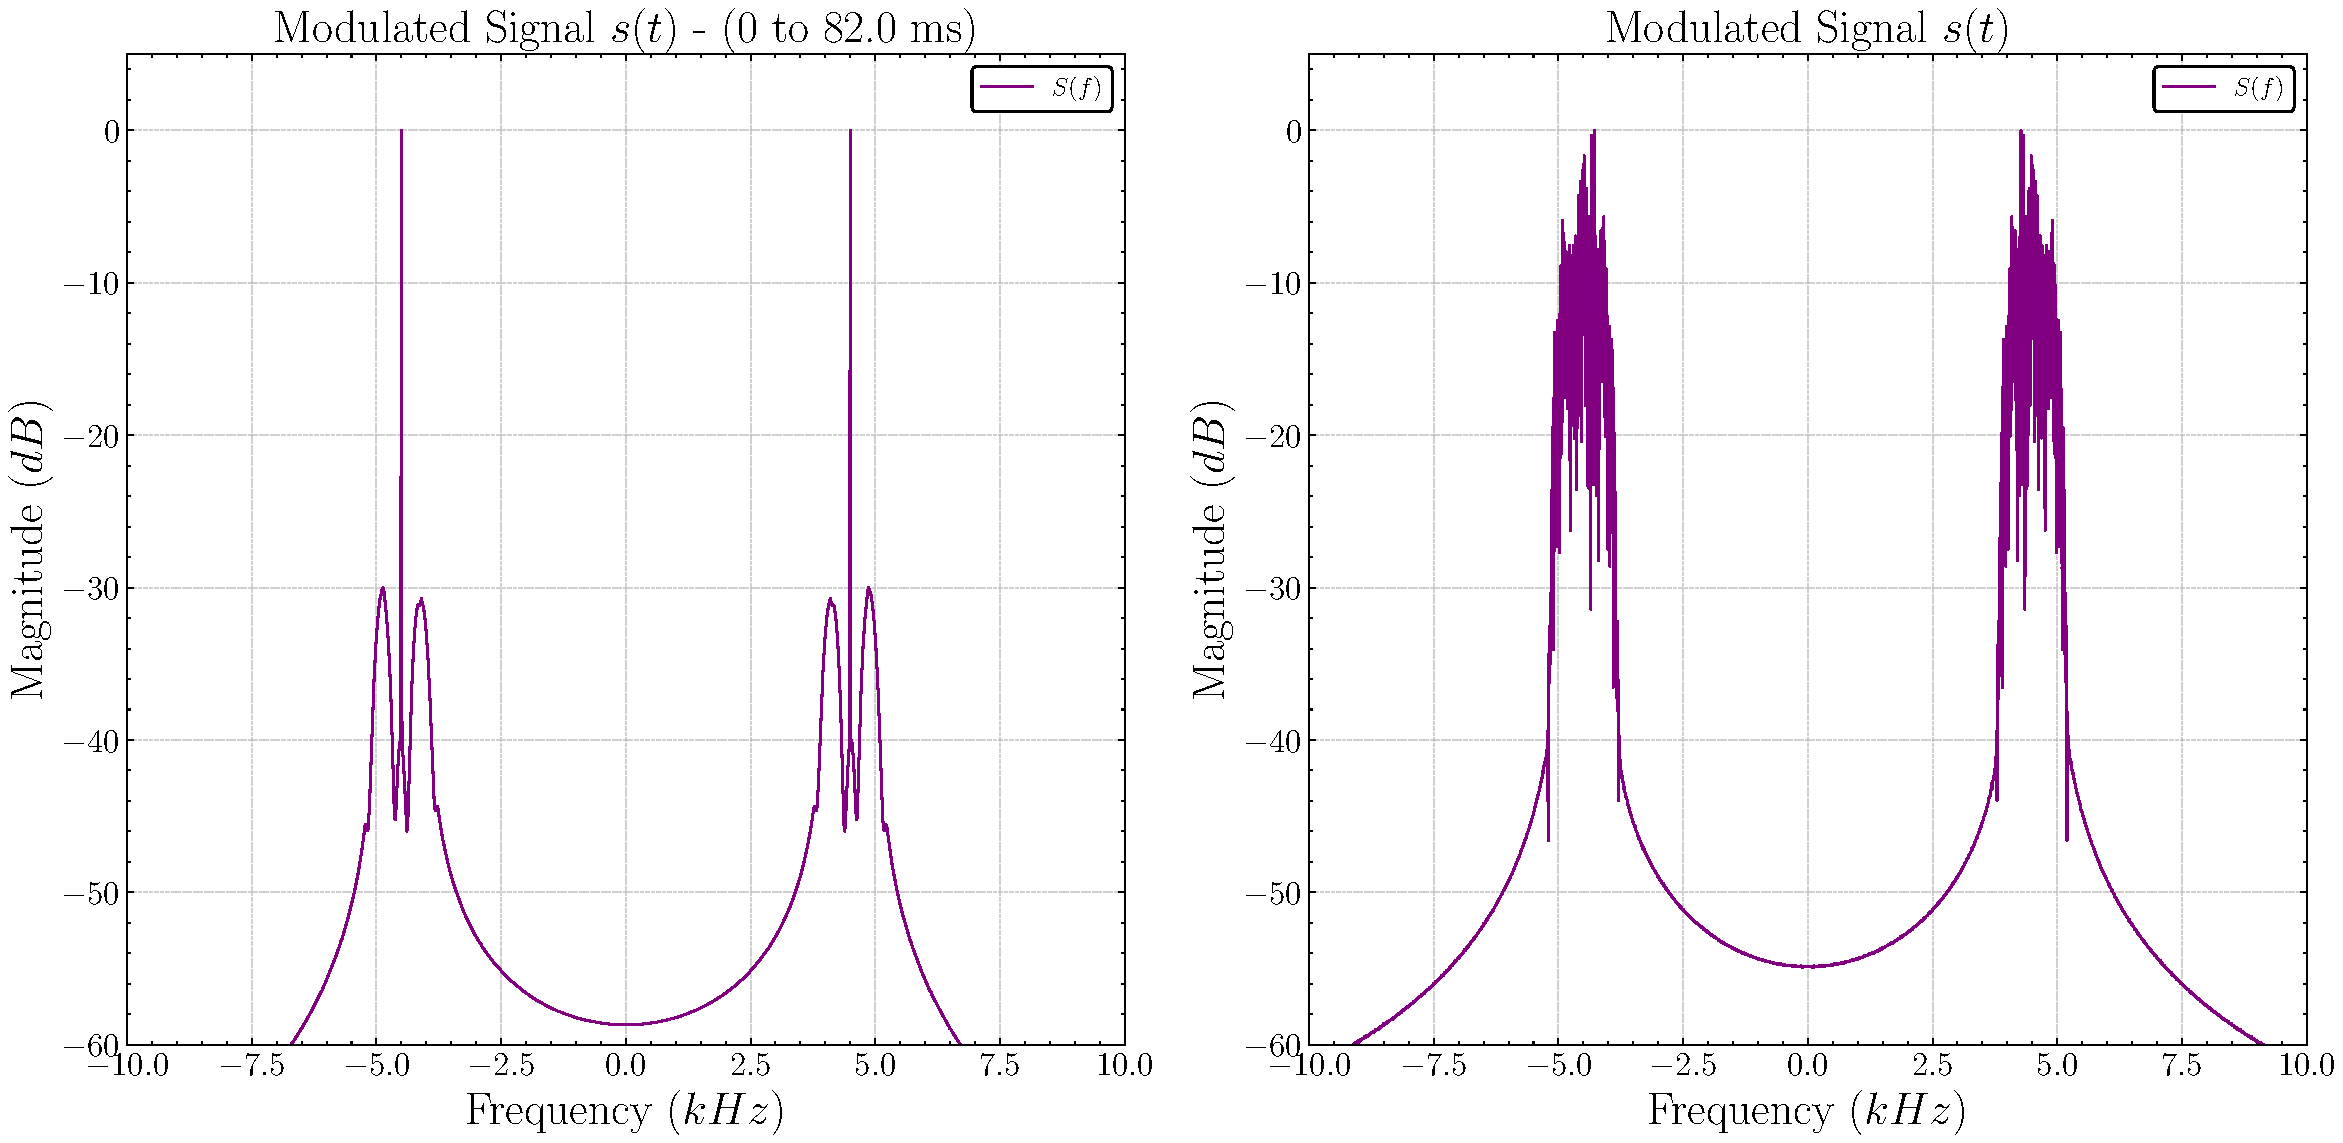
\includegraphics[width=\linewidth]{assets/cap3/transmitter_modulator_portadora.pdf}
\end{figure}

\section{CANAL E ADIÇÃO DE RUÍDO}\label{sec:canal}


Após a modulação do sinal \gls{st} em banda passante, o próximo passo é a transmissão através do canal de comunicação, que permite a adição de múltiplas transmissões simultâneas e a introdução de ruído \gls{AWGN} ao sinal transmitido. O diagrama de blocos do canal é ilustrado na \autoref{fig:channel_diagram}.

\begin{figure}[H]
	\centering
	\caption{Diagrama de blocos do canal}\label{fig:channel_diagram}
	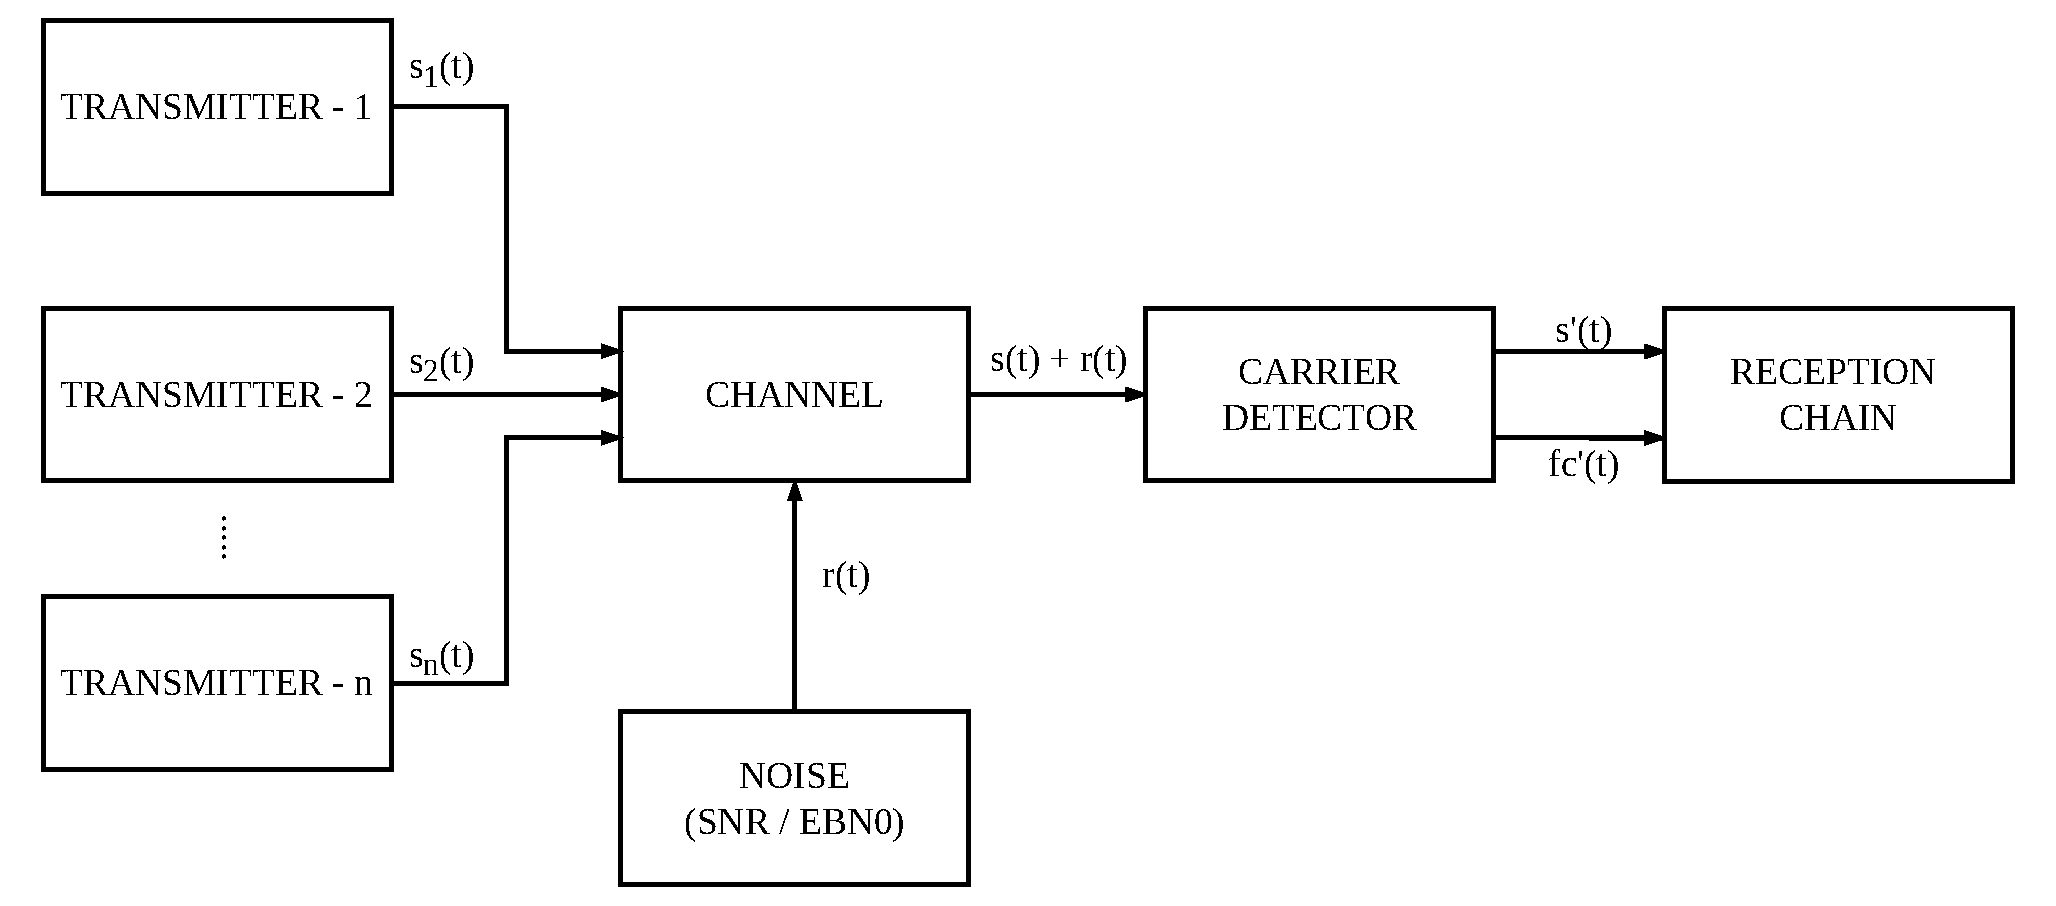
\includegraphics[width=\linewidth]{assets/diagrams/channel.pdf}
\end{figure}

\subsection{Modelo de canal}\label{sec:modelo_canal}

O modelo de canal é instânciado com base na \gls{fs} e na duração desejada para o canal, padrão $1$ segundo. A partir disto, é possivel calcular a quantidade de amostras necessárias para compor o canal, e então criar um vetor de zeros com o tamanho adequado, que servirá como base para a adição das transmissões. O modelo de canal é ilustrado na \autoref{fig:channel_time}.

\begin{figure}[H]
	\centering
	\caption{Adição de múltiplas transmissões no canal}\label{fig:channel_time}
	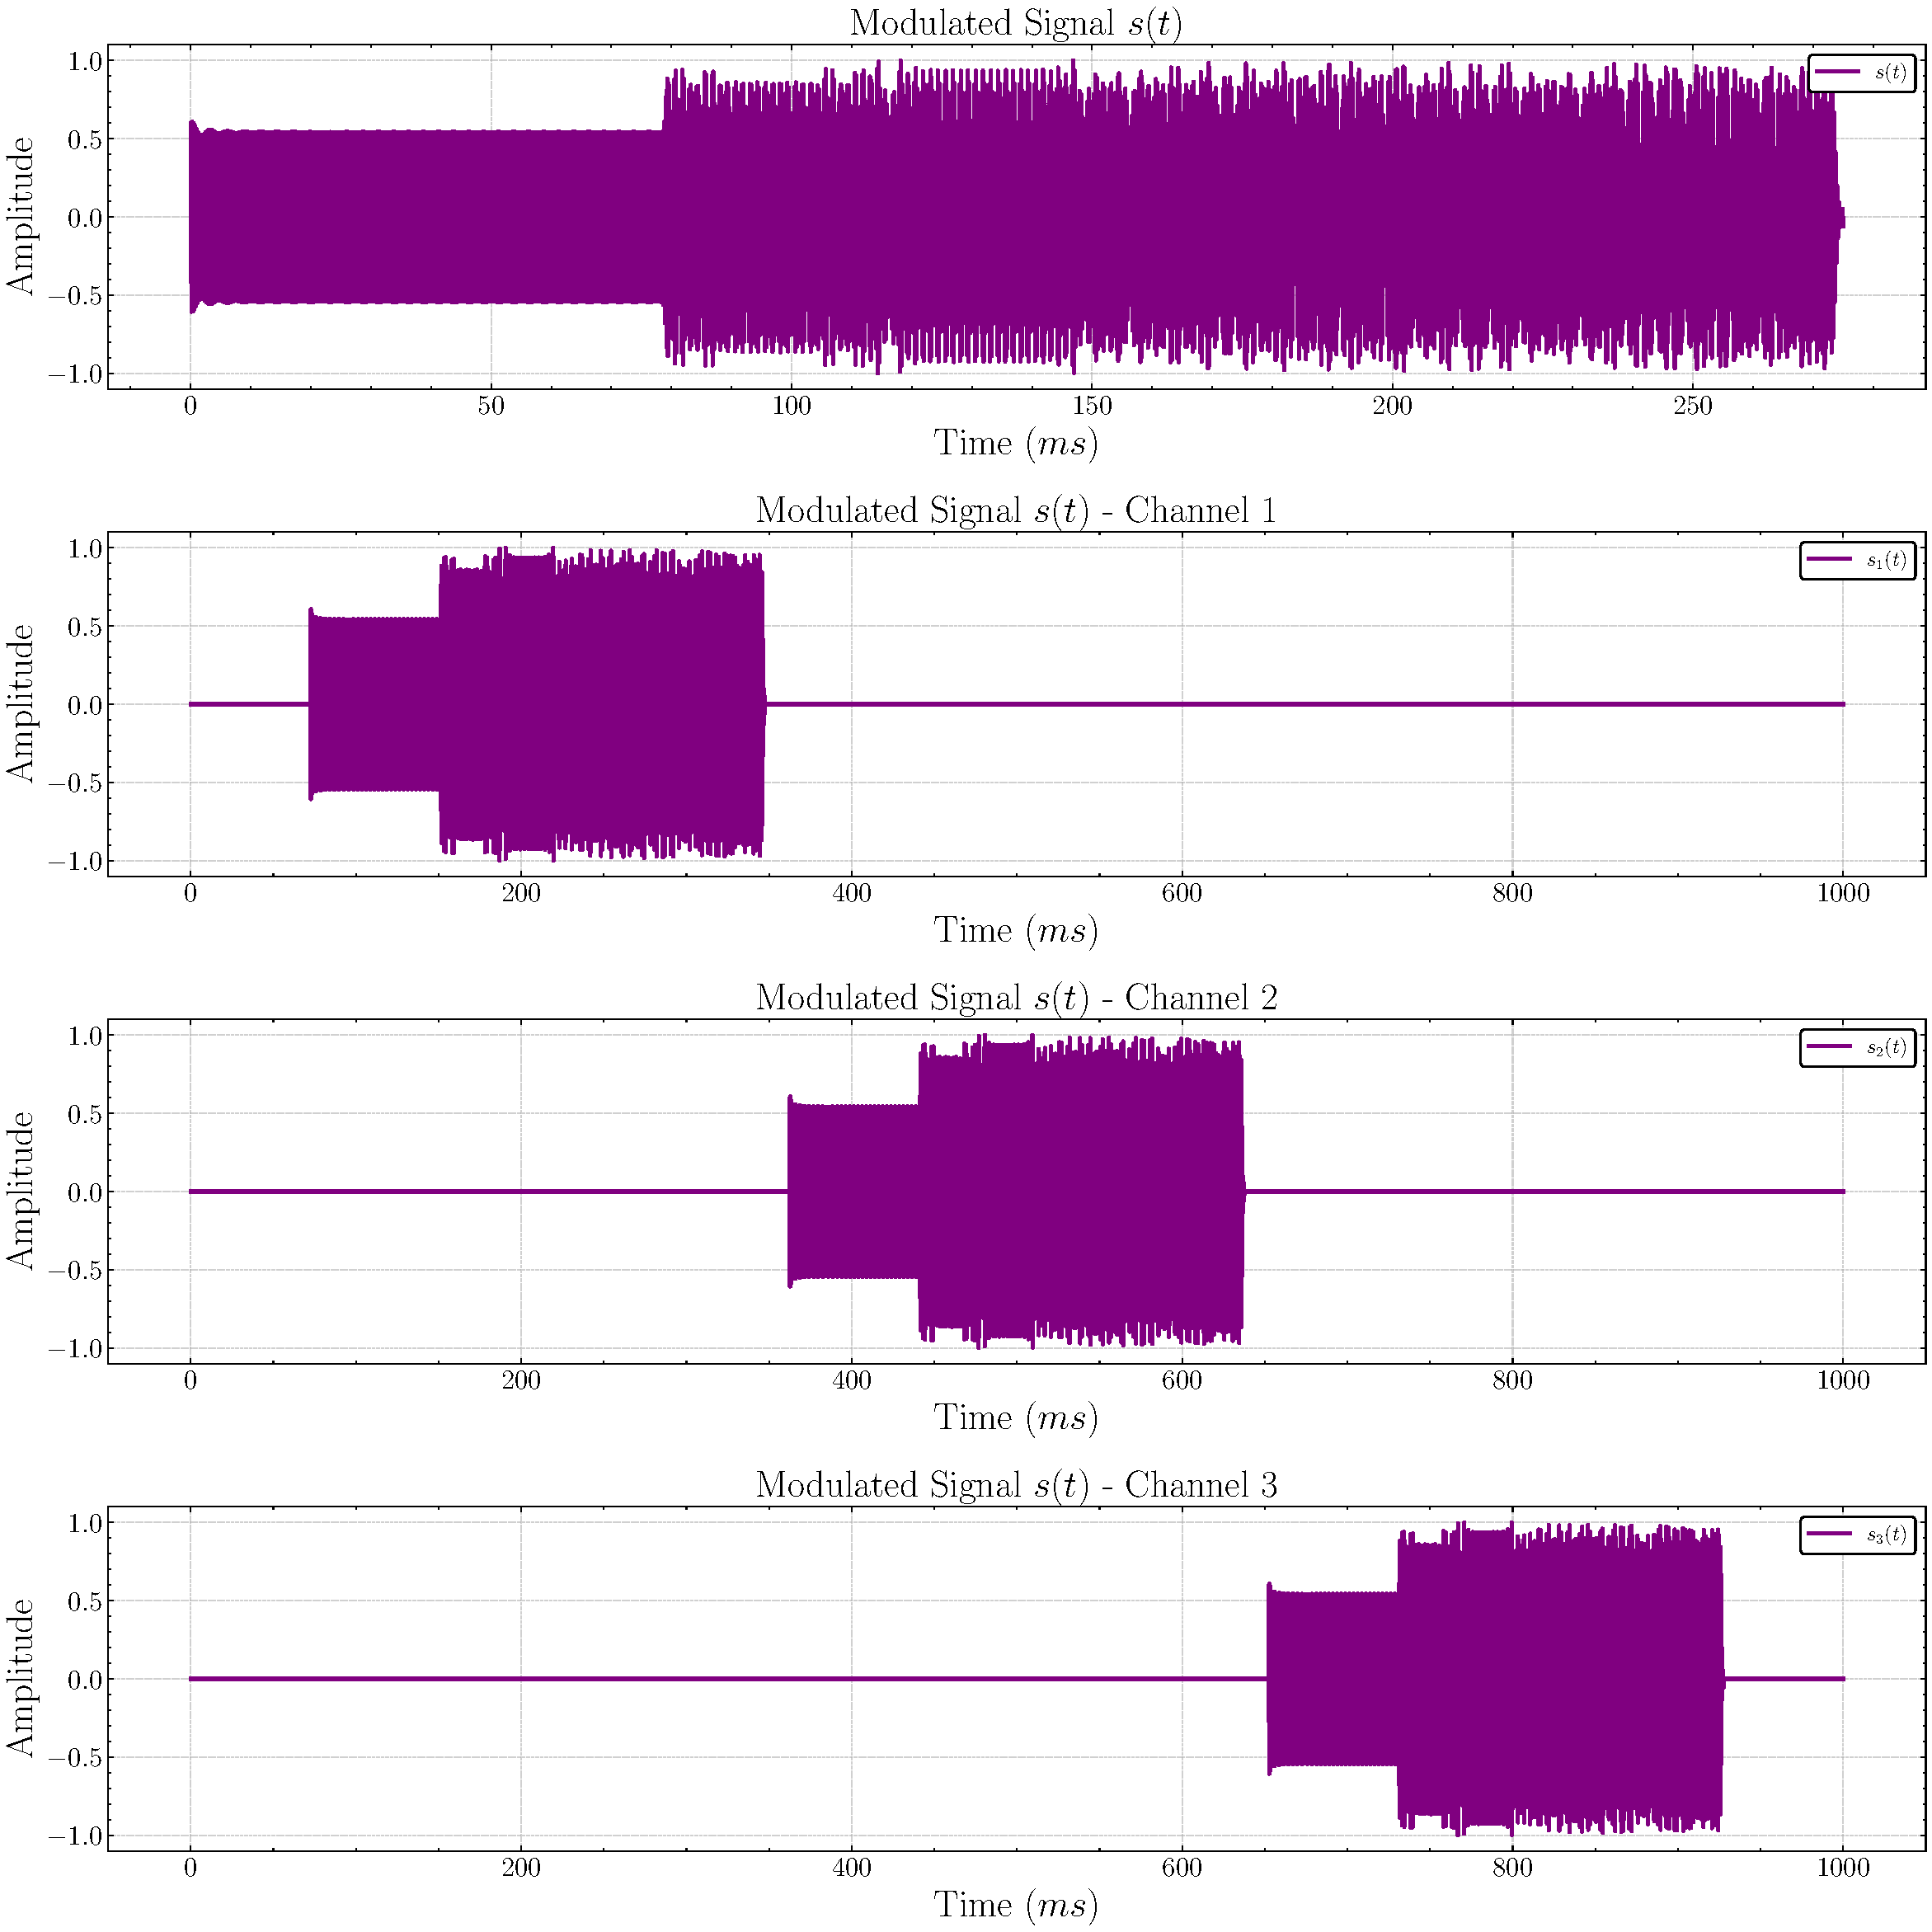
\includegraphics[width=\linewidth]{assets/cap3/example_channel_time_subchannels.pdf}
\end{figure}

Em seguida, cada transmissão é adicionada ao canal junto a fator de posição desejado, fator que pode variar entre $0$ e $1$, onde $0$ representa o início do canal e $1$ representa o final do canal. A posição de cada transmissão é calculada com base no fator de posição e na quantidade total de amostras do canal. 

\subsection{Geração de ruído AWGN}\label{sec:geracao_ruido}

Uma vez com as transmissões adicionadas ao canal, o próximo passo é a geração do ruído \gls{AWGN} com base na \gls{SNR} ou \gls{EbN0} desejada. O ruído é gerado como um vetor de números aleatórios com distribuição normal, com média zero e variância calculada com base no tipo de ruído utilizado e na potência do sinal transmitido. O calculo da \gls{sigma2} utilizada na geração do ruído \gls{SNR} pode ser expresso como

\begin{equation}
    \sigma^2 = \frac{\mathbb{E}\!\left[ |s(t)|^2 \right]}{10^{\frac{\mathrm{SNR}_{dB}}{10}}}
\end{equation}

\noindent Onde $\mathbb{E}\!\left[ |s(t)|^2 \right]$ é a potência do sinal transmitido e $\mathrm{SNR}_{dB}$ é a relação sinal-ruído em decibéis. A geração e adição do ruído \gls{rt} ao sinal \gls{st} é ilustrada na \autoref{fig:add_noise_time}.

\begin{figure}[H]
	\centering
	\caption{Adição de ruído ao canal}\label{fig:add_noise_time}
	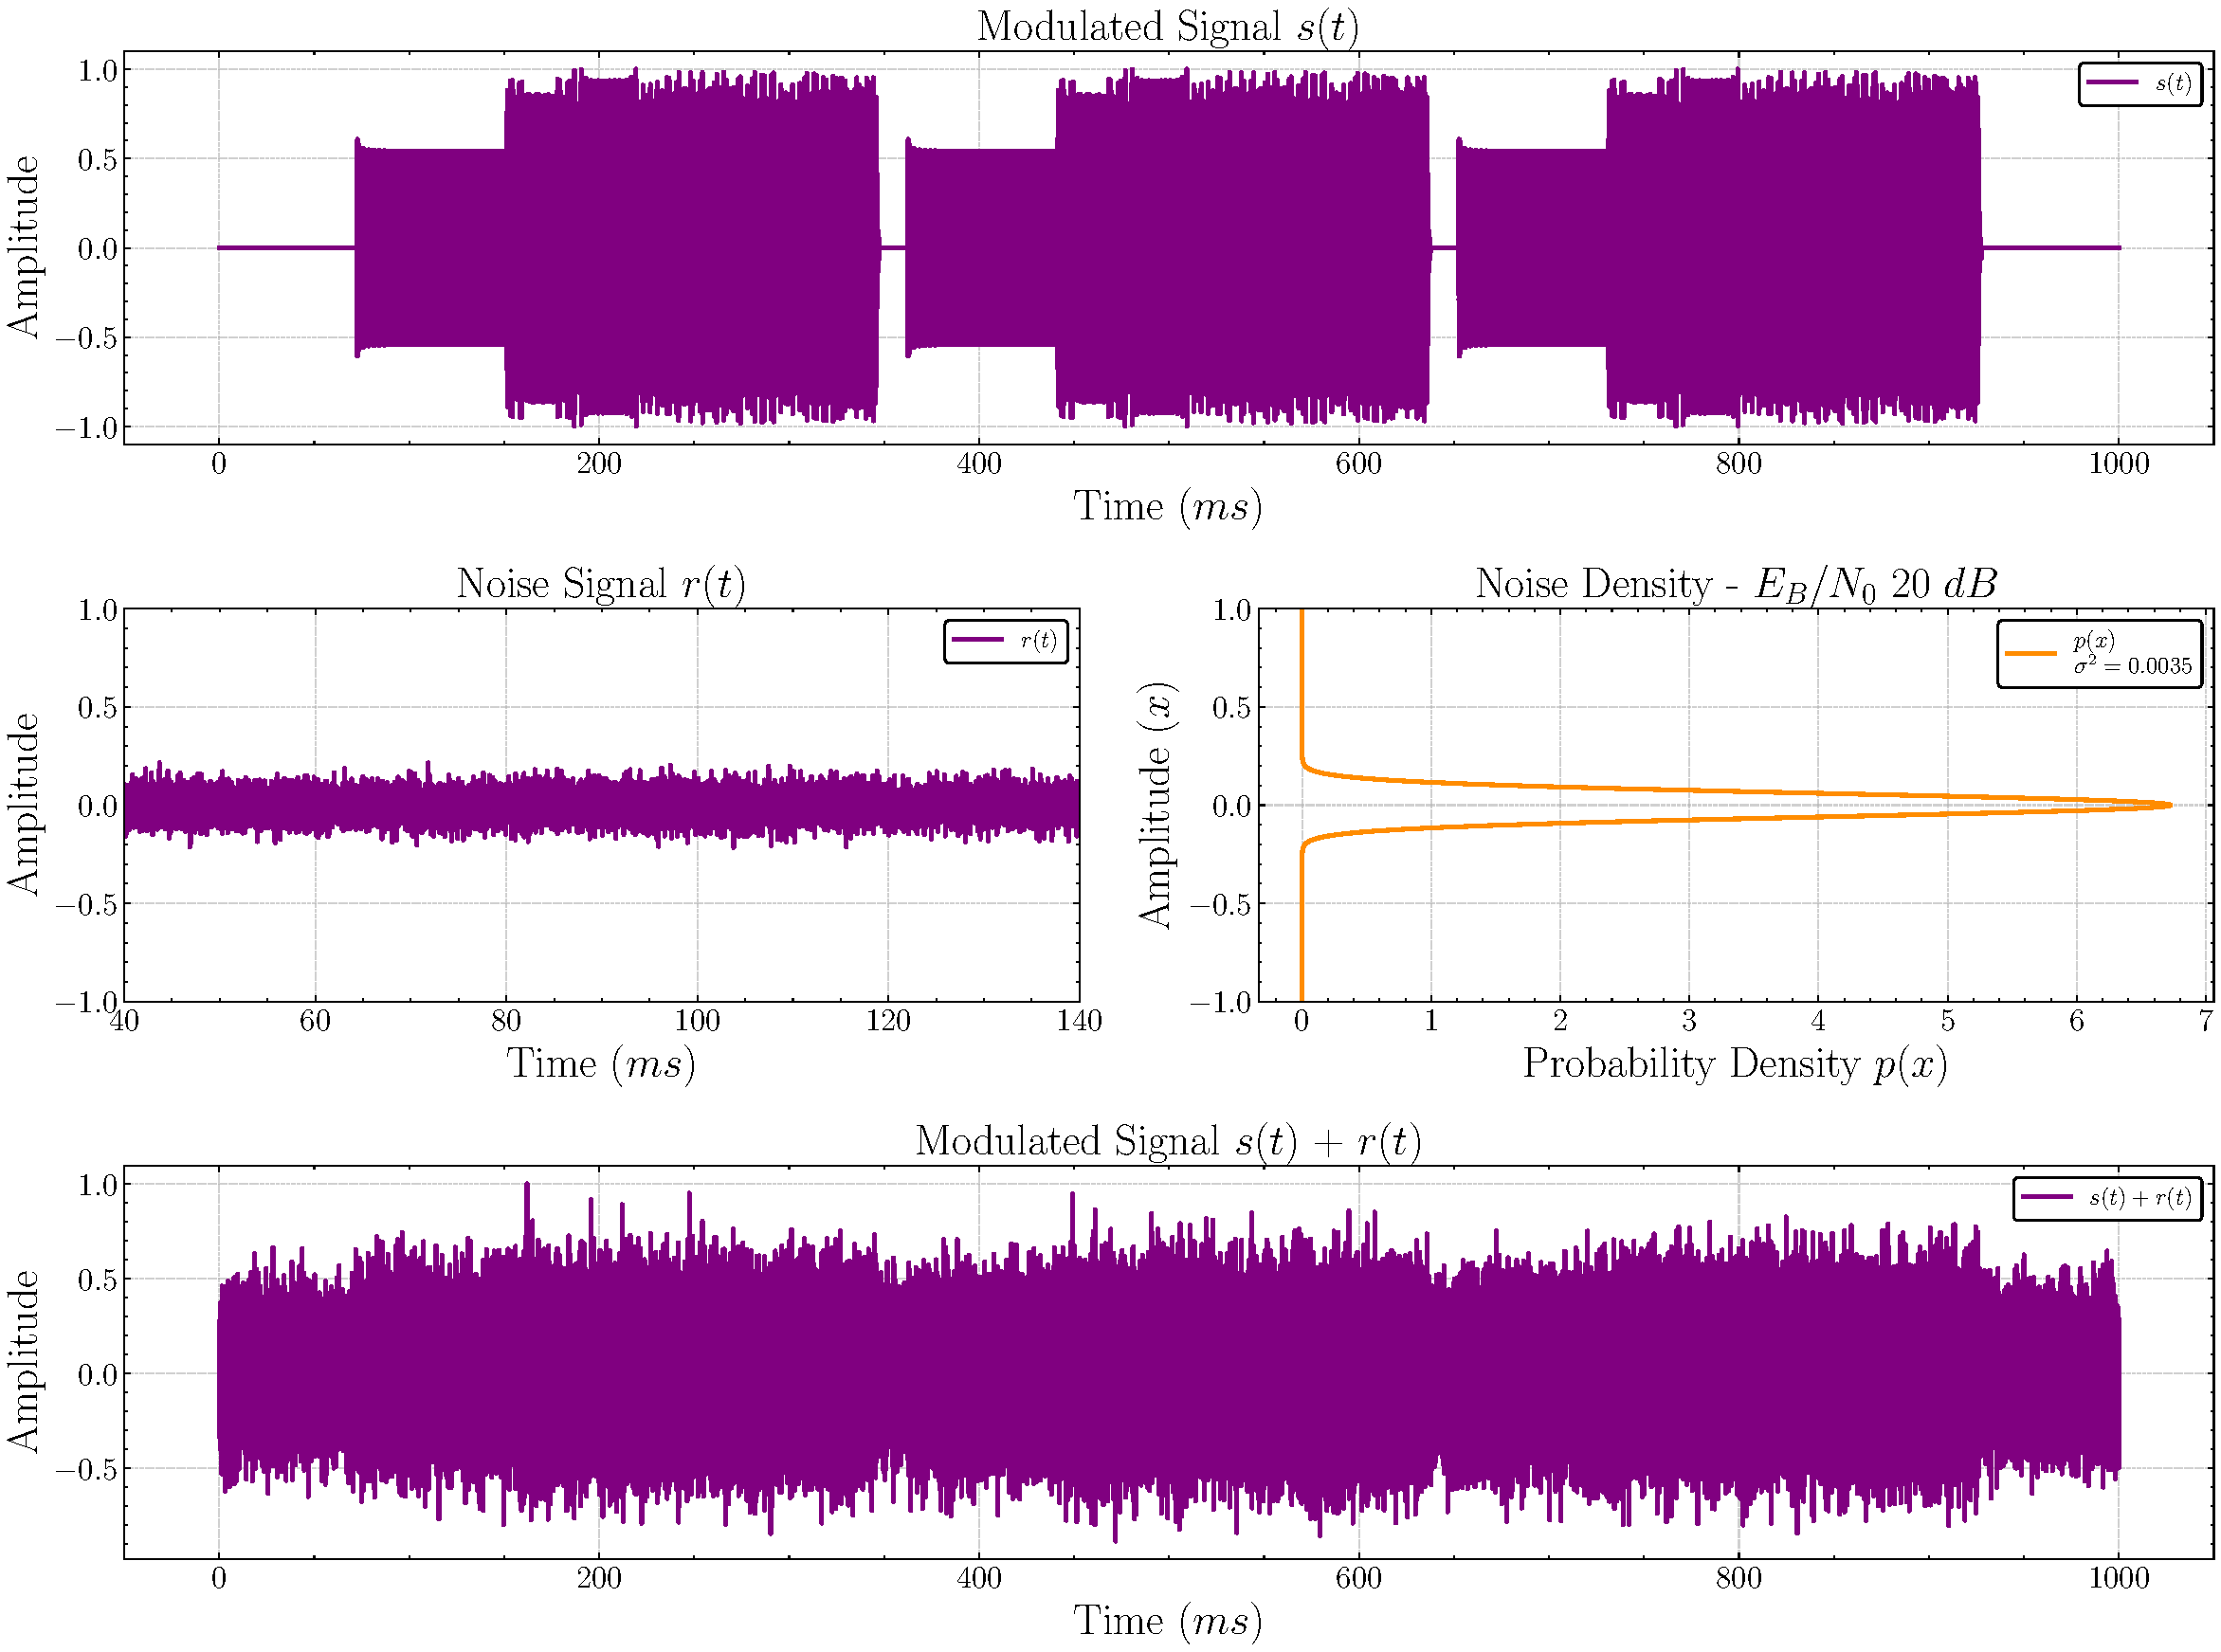
\includegraphics[width=\linewidth]{assets/cap3/example_channel_time_channel.pdf}
\end{figure}

\section{DETECÇÃO DE PORTADORA}\label{sec:detector}

Com as múltiplas transmissões e o ruído adicionados ao canal, o próximo passo é a detecção das portadoras presentes no canal para posterior recepção. A detecção de portadora é realizada através de um processo de segmentação do sinal recebido em segmentos \gls{xn}, análise do espectro de cada segmento para identificação de componentes com potência acima de um limiar definido \gls{Pt}, e decisão sobre quais componentes serão consideradas como portadoras válidas. O diagrama de blocos do detector é ilustrado na \autoref{fig:detector_diagram}.

\begin{figure}[H]
	\centering
	\caption{Diagrama de blocos da detecção de portadora}\label{fig:detector_diagram}
	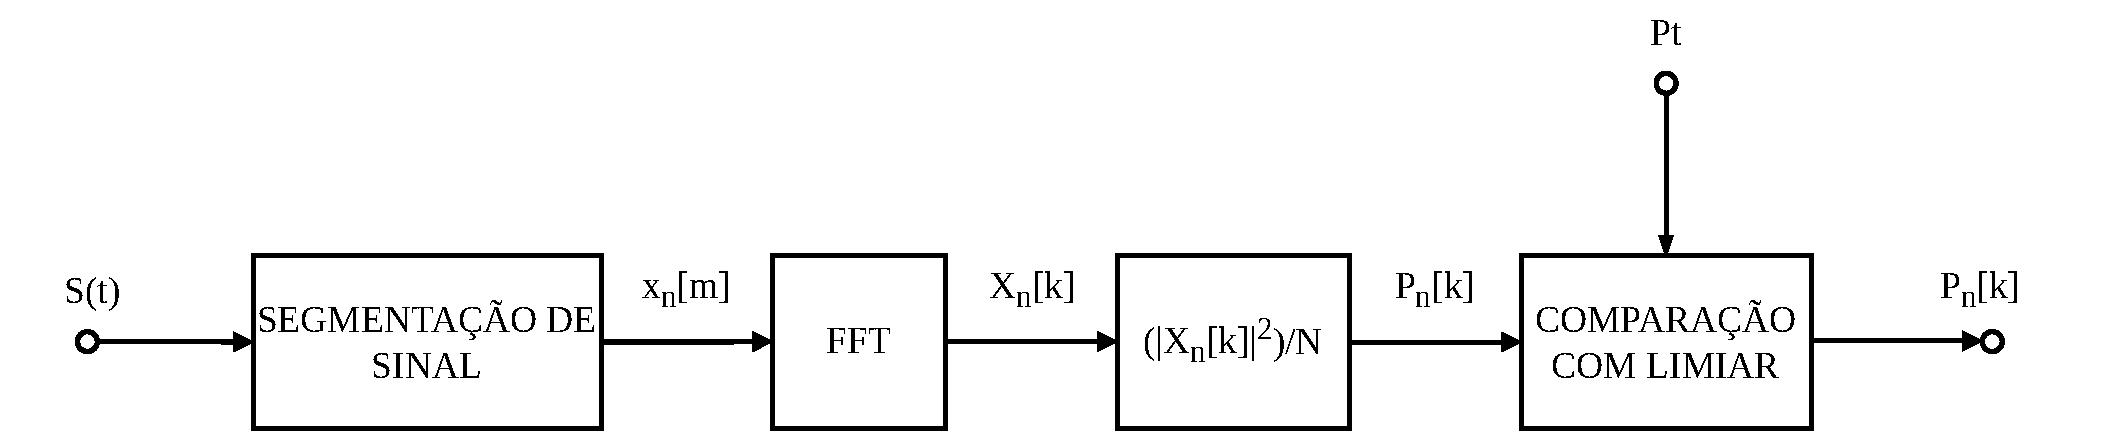
\includegraphics[width=\linewidth]{assets/diagrams/detector.pdf}
\end{figure}

\subsection{Segmentação do sinal recebido}\label{sec:segmentacao}

O primeiro passo na detecção de portadora é a segmentação do sinal recebido \gls{rt} em segmentos \gls{xn} de duração \gls{Tm}, conforme detalhado na seção \ref{sec:detector}. Cada segmento é então analisado individualmente para identificar a potência \gls{Pnk} de cada componente \gls{k} de cada segmento \gls{m}, formando assim uma matriz $m \times k$, podendo ser representado como um diagrama waterfall, conforme ilustrado na \autoref{fig:waterfall}.

\begin{figure}[H]
	\centering
	\caption{Diagrama de waterfall do canal}\label{fig:waterfall}
	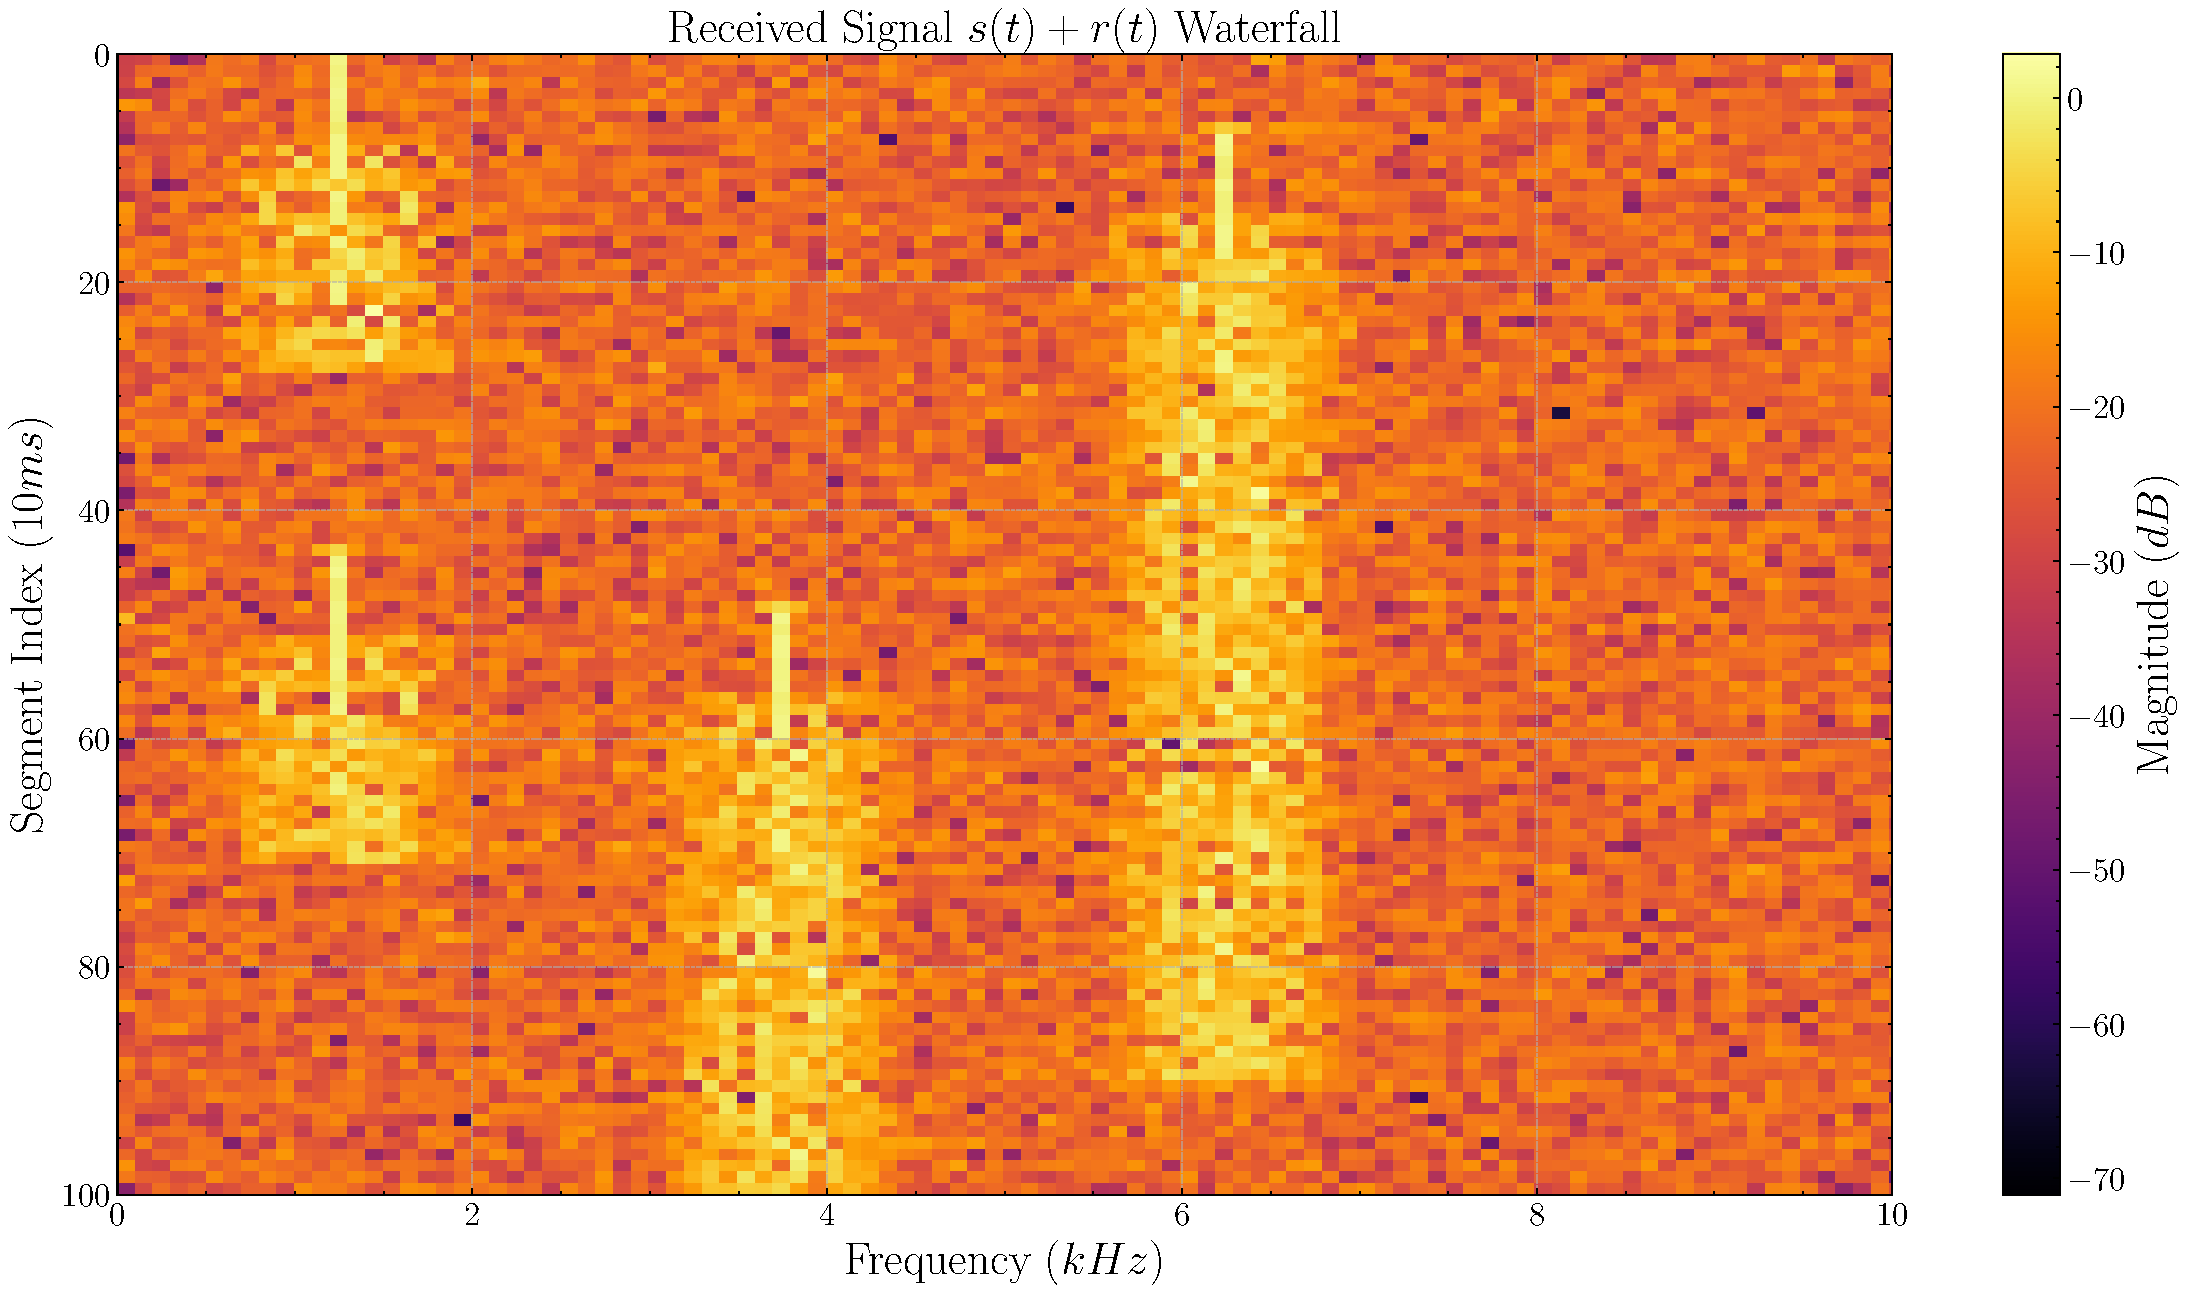
\includegraphics[width=\linewidth]{assets/cap3/example_detector_waterfall.pdf}
\end{figure}

Na \ref{fig:waterfall} é possível observar claramente a presença das transmissões realizadas, além disso, nota-se que no inicio de cada transmissão a uma sequência de altas componentes, formando uma linha, que corresponde ao período de portadora pura \gls{Pd}, conforme detalhado na seção \ref{sec:qpsk}.

\subsection{Detecção de componentes no espectro}\label{sec:comparacao_potencia}

Para cada segmento \gls{xn}, as componentes \gls{Pnk} são comparadas com o limiar de potência \gls{Pt}, e aquelas que apresentarem potência acima do limiar são consideradas como componentes detectadas. O resultado dessa comparação é uma matriz $m \times k$, onde cada elemento indica se a componente \gls{k} do segmento \gls{m} foi detectada ou não. A detecção de componentes no espectro com base em \gls{Pt} é ilustrada na \autoref{fig:freq_detection}.

\begin{figure}[H]
	\centering
	\caption{Detecção de componentes no espectro com base em $P_t$}\label{fig:freq_detection}
	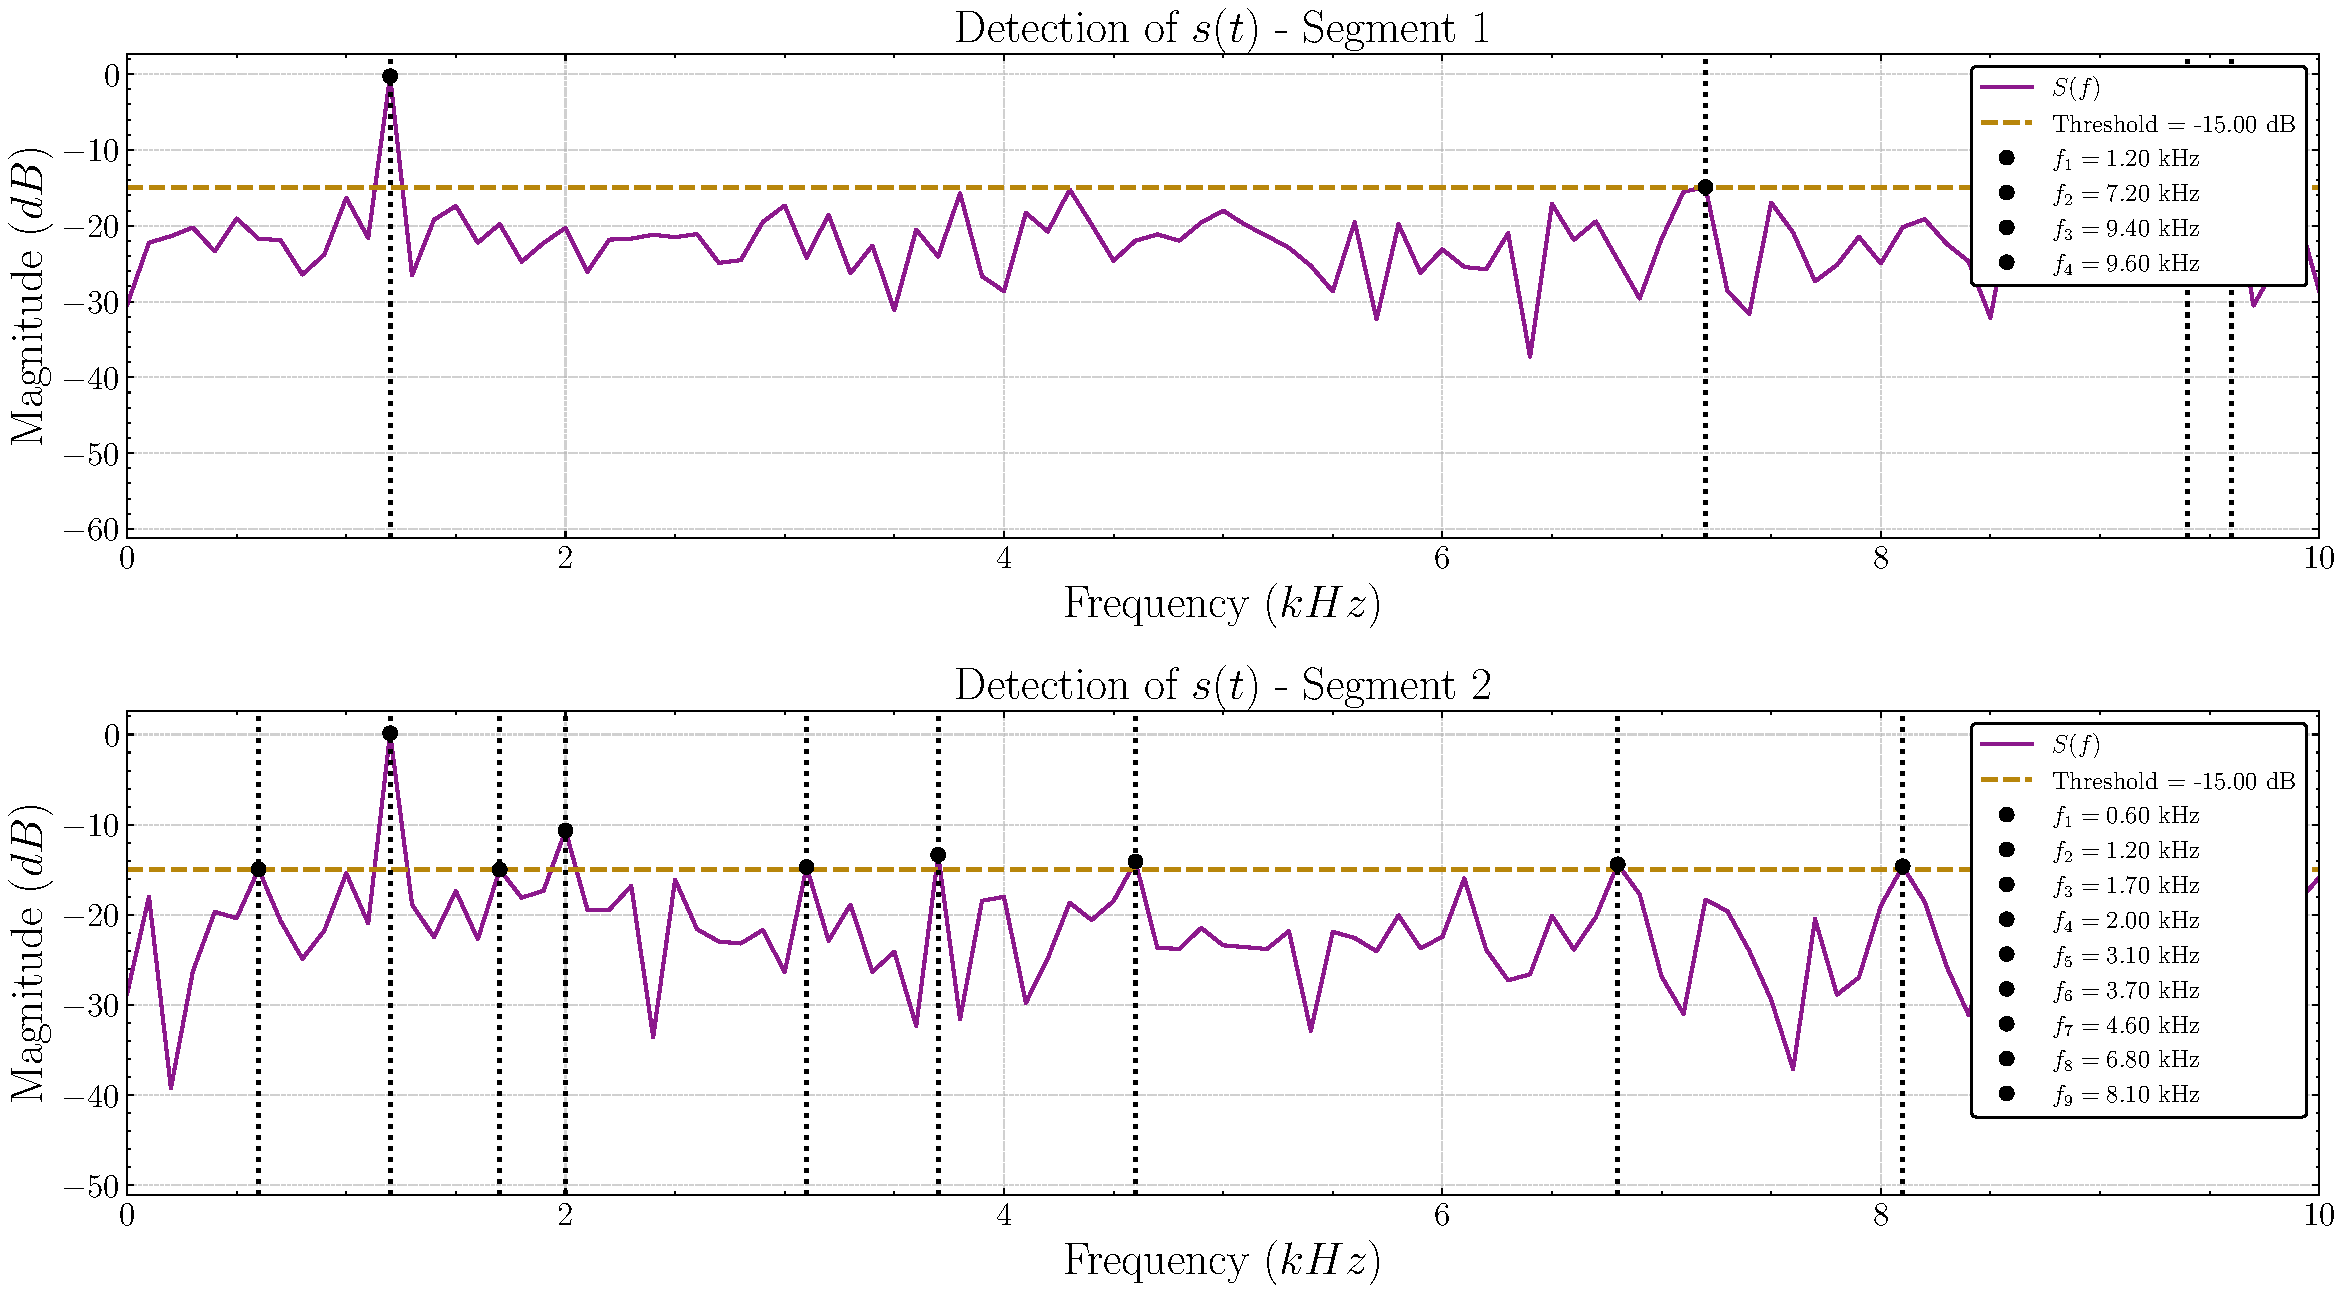
\includegraphics[width=\linewidth]{assets/cap3/example_detector_freq.pdf}
\end{figure}

Além disso, quando uma componente é detectada múltiplas vezes concecutivas, essa componente é considerada como "confirmada", ou seja, é uma componente que provavelmente corresponde a uma portadora válida, a quantidade de vezes consecutivas que uma componente deve ser detectada para ser considerada como confirmada é definida pelo parâmetro \gls{Nc}. A matriz de componentes detectadas e confirmadas pode ser representada como um diagrama waterfall, conforme ilustrado na \autoref{fig:waterfall_detection}.

\begin{figure}[H]
	\centering
	\caption{Diagrama de waterfall de detecção do canal}\label{fig:waterfall_detection}
	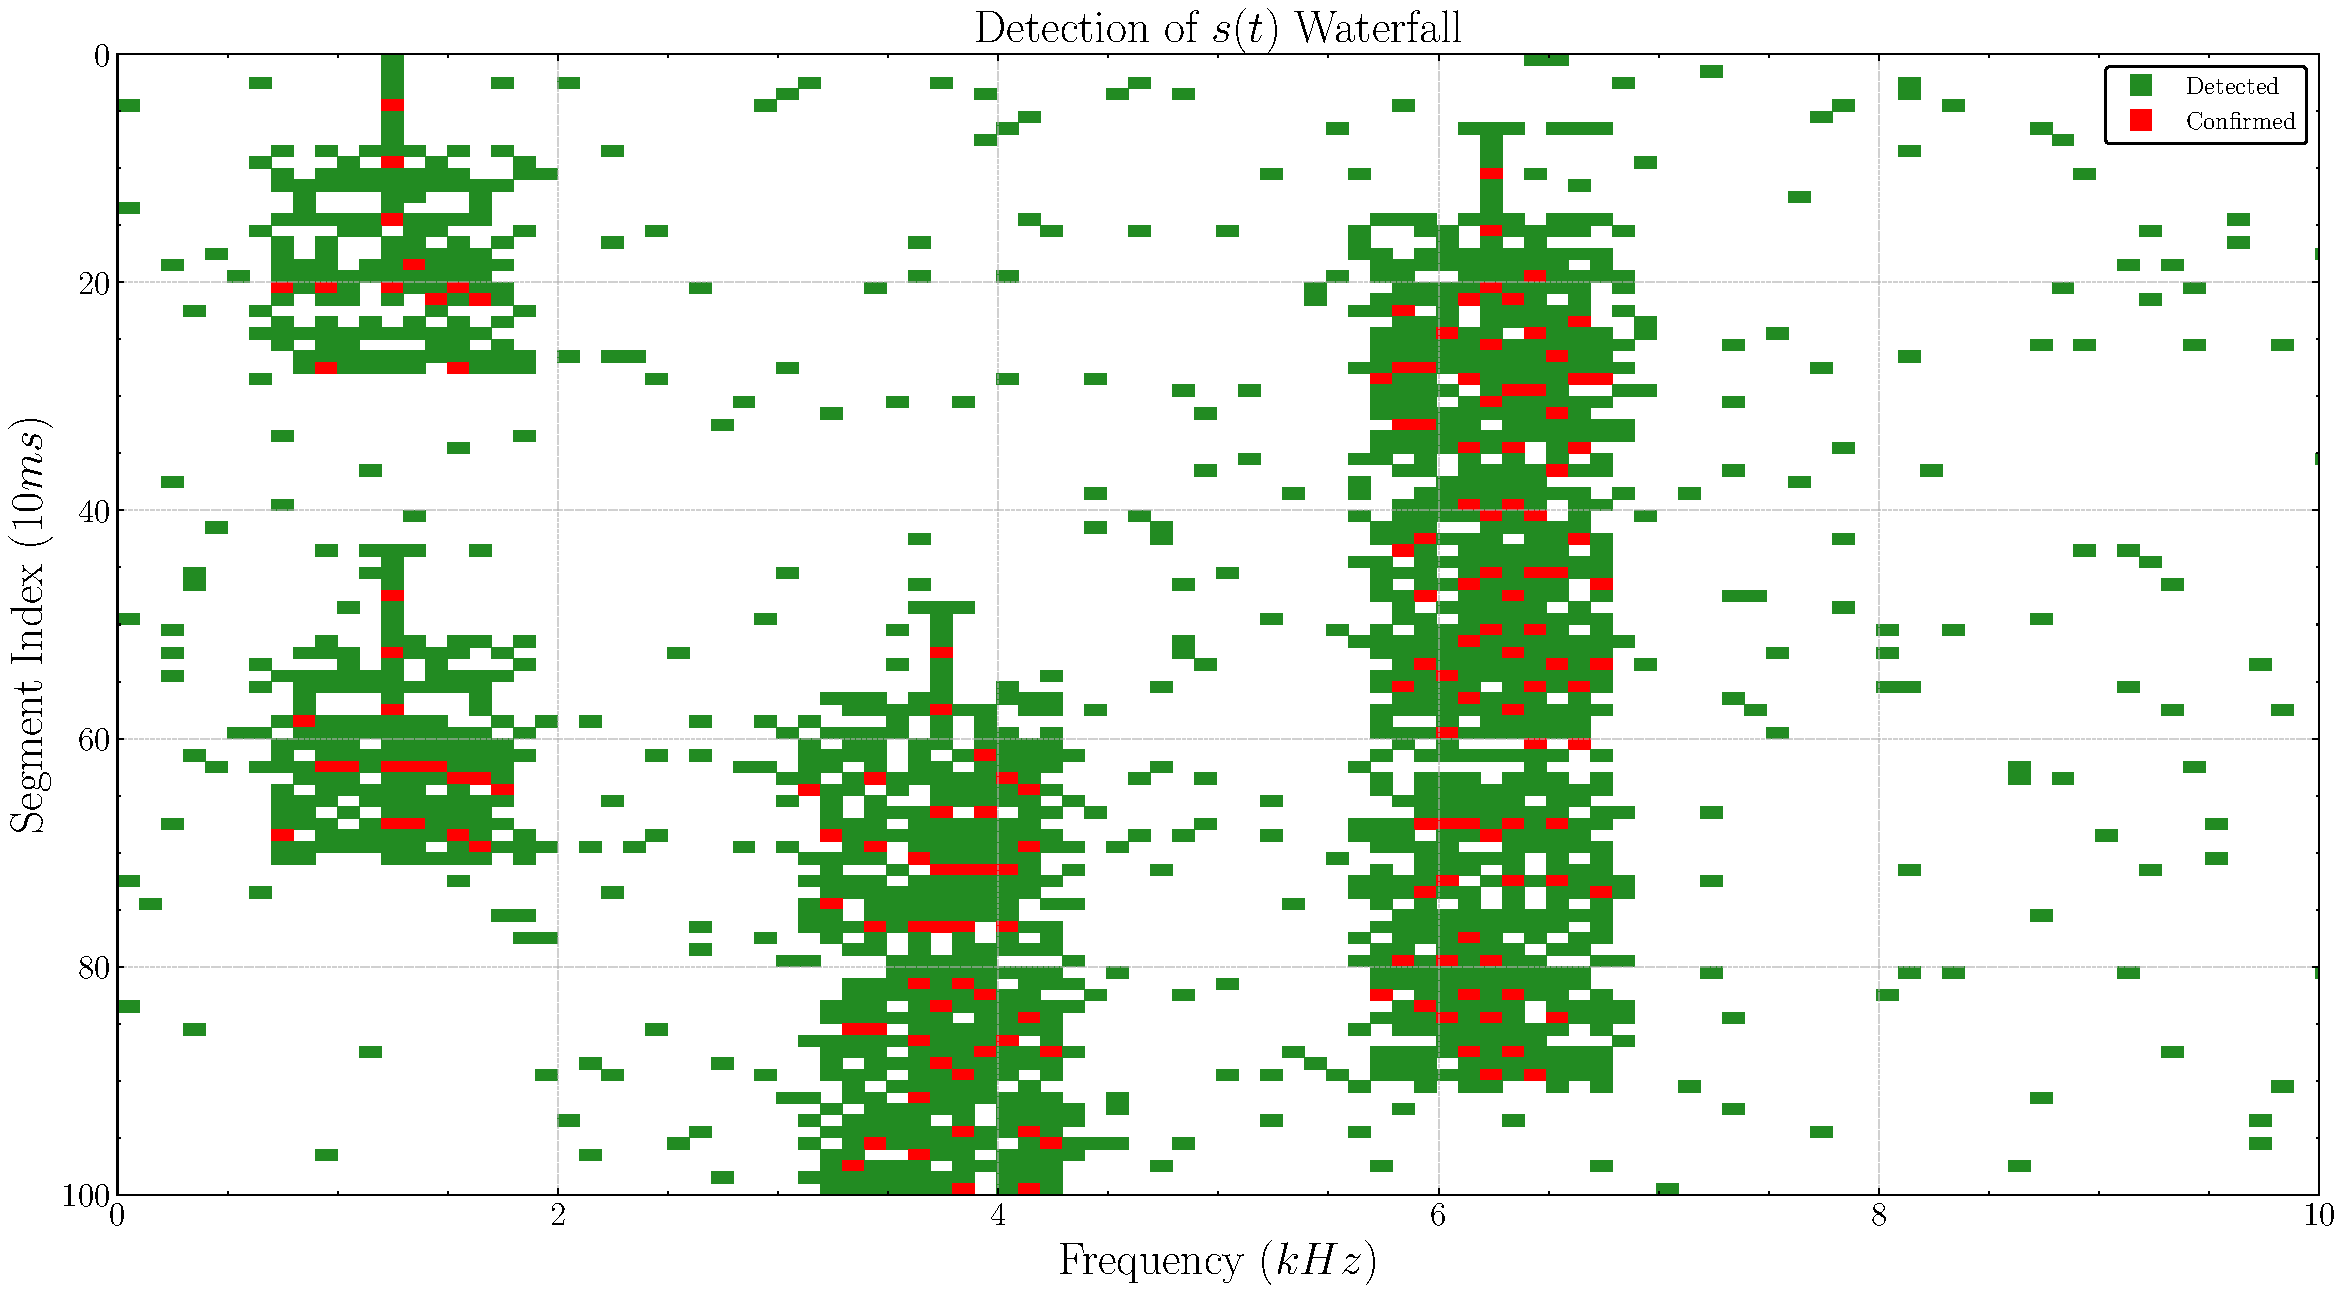
\includegraphics[width=\linewidth]{assets/cap3/example_detector_waterfall_detection.pdf}
\end{figure}

No simulador, \gls{Nc} é fixado em $4$, por ser metade do comprimento da portadora pura, entretanto, quanto maior o valor de \gls{Nc}, maior a certeza de que a componente detectada é realmente uma portadora válida portanto maior a tolerância da decisão a \gls{Pt} mais baixos, porém, isso também pode aumentar falhas de detecção, caso o período de amostragem do detector não seja suficiente para conformar a transmissão.

\subsection{Decisão de componentes detectadas}\label{sec:decisao}

Com base na matriz de componentes confirmadas, o próximo passo é a decisão sobre quais componentes serão efetivamente consideradas como portadoras válidas para recepção. A decisão é baseada na continuidade da detecção de componentes ao longo dos segmentos, assim a primeira componente confirmada sobre a frequência \gls{fcprime} é considerada como o inicio de uma transmissão, a partir dela, é aplicado um span, isto é, um intervalo de amostras no mesmo segmento onde são ignoradas novas detecções, esse span tem largura \gls{W}, e é aplicado consecutivamente até o fim das detecções sobre a frequência \gls{fcprime}. A decisão de componentes detectadas é ilustrada na \autoref{fig:waterfall_decision}.

\begin{figure}[H]
	\centering
	\caption{Diagrama de waterfall de decisão do canal}\label{fig:waterfall_decision}
	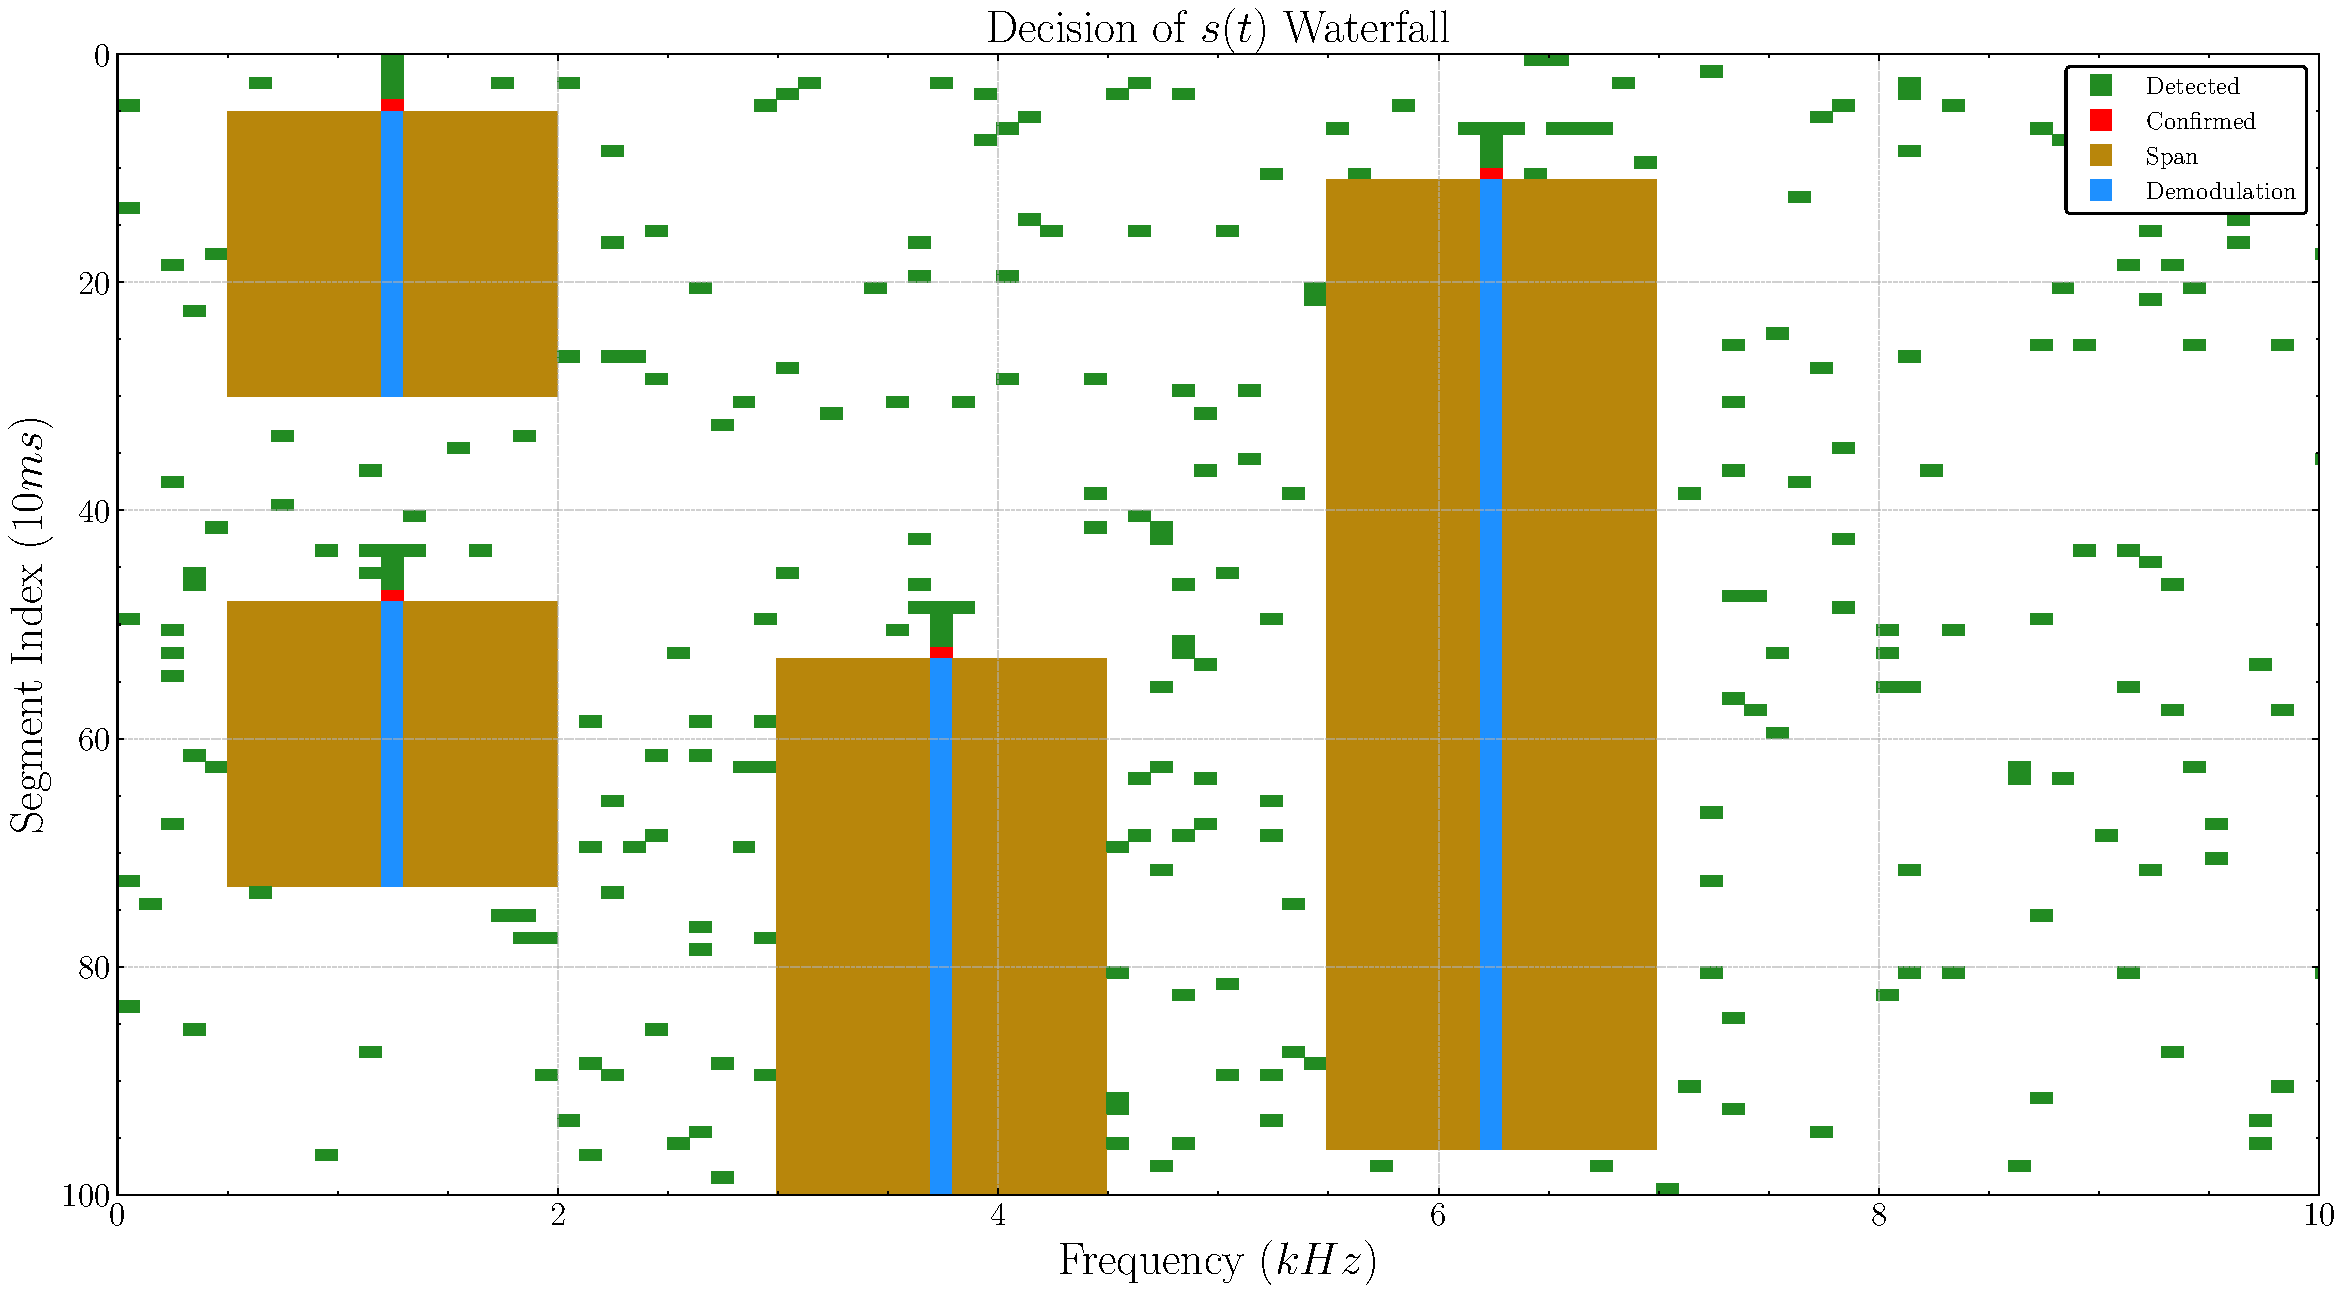
\includegraphics[width=\linewidth]{assets/cap3/example_detector_waterfall_decision.pdf}
\end{figure}

\subsection{Segmentação do sinal recebido para recepção}\label{sec:segmentacao_recepcao}

Para cada componente \gls{fcprime} decidida como portadora válida, tendo seu segmento de inicio e seu segmento de fim, o próximo passo é a segmentação do sinal recebido \gls{st} para recepção em segmentos de sinal \gls{stprime}. Cada segmento \gls{stprime} é então processado individualmente na cadeia de recepção com sua respectiva \gls{fcprime}, conforme detalhado na seção \ref{sec:recepcao}. O proceso de segmentação do sinal recebido para recepção é apresentado no código de exemplo \ref{cod:detector}.

\lstinputlisting[language=python,caption={Recepção de sinal $s'(t)$},label=cod:detector]{codigo/detector.py}

\section{CADEIA DE RECEPÇÃO}\label{sec:recepcao}    

A cadeia de recepção é responsável por recuperar o datagrama transmitido a partir do sinal recebido \gls{stprime}, que foi segmentado e identificado como uma portadora válida na etapa de detecção de portadora, conforme detalhado na seção \ref{sec:detector}. A cadeia de recepção é dividida em demodulação em banda base, filtragem, sincronização de símbolos, decisão de símbolos e recuperação do datagramam conforme apresentado na seção \ref{sec:receptor}

\subsection{Demodulação banda base}\label{sec:demodulacao}

O primeiro passo na cadeia de recepção é a demodulação do sinal recebido \gls{stprime} para retornar o sinal para banda base. Para isso, é necessário injetar uma componente senoidal e cossenoidal no \gls{stprime} com a mesma frequência \gls{fcprime} da portadora detectada, fazendo com que o sinal seja transladado, isto é, deslocado para banda base formando as componentes \gls{dXprime} e \gls{dYprime}, o processo de demodulação também faz com que uma componente identica seja gerada na frequência $2 \cdot \gls{fcprime}$, esse processo é ilustrado na \autoref{fig:receiver_demodulator}.

\begin{figure}[H]
	\centering
	\caption{Demodulação banda base dos canais $I$ e $Q$}\label{fig:receiver_demodulator}
	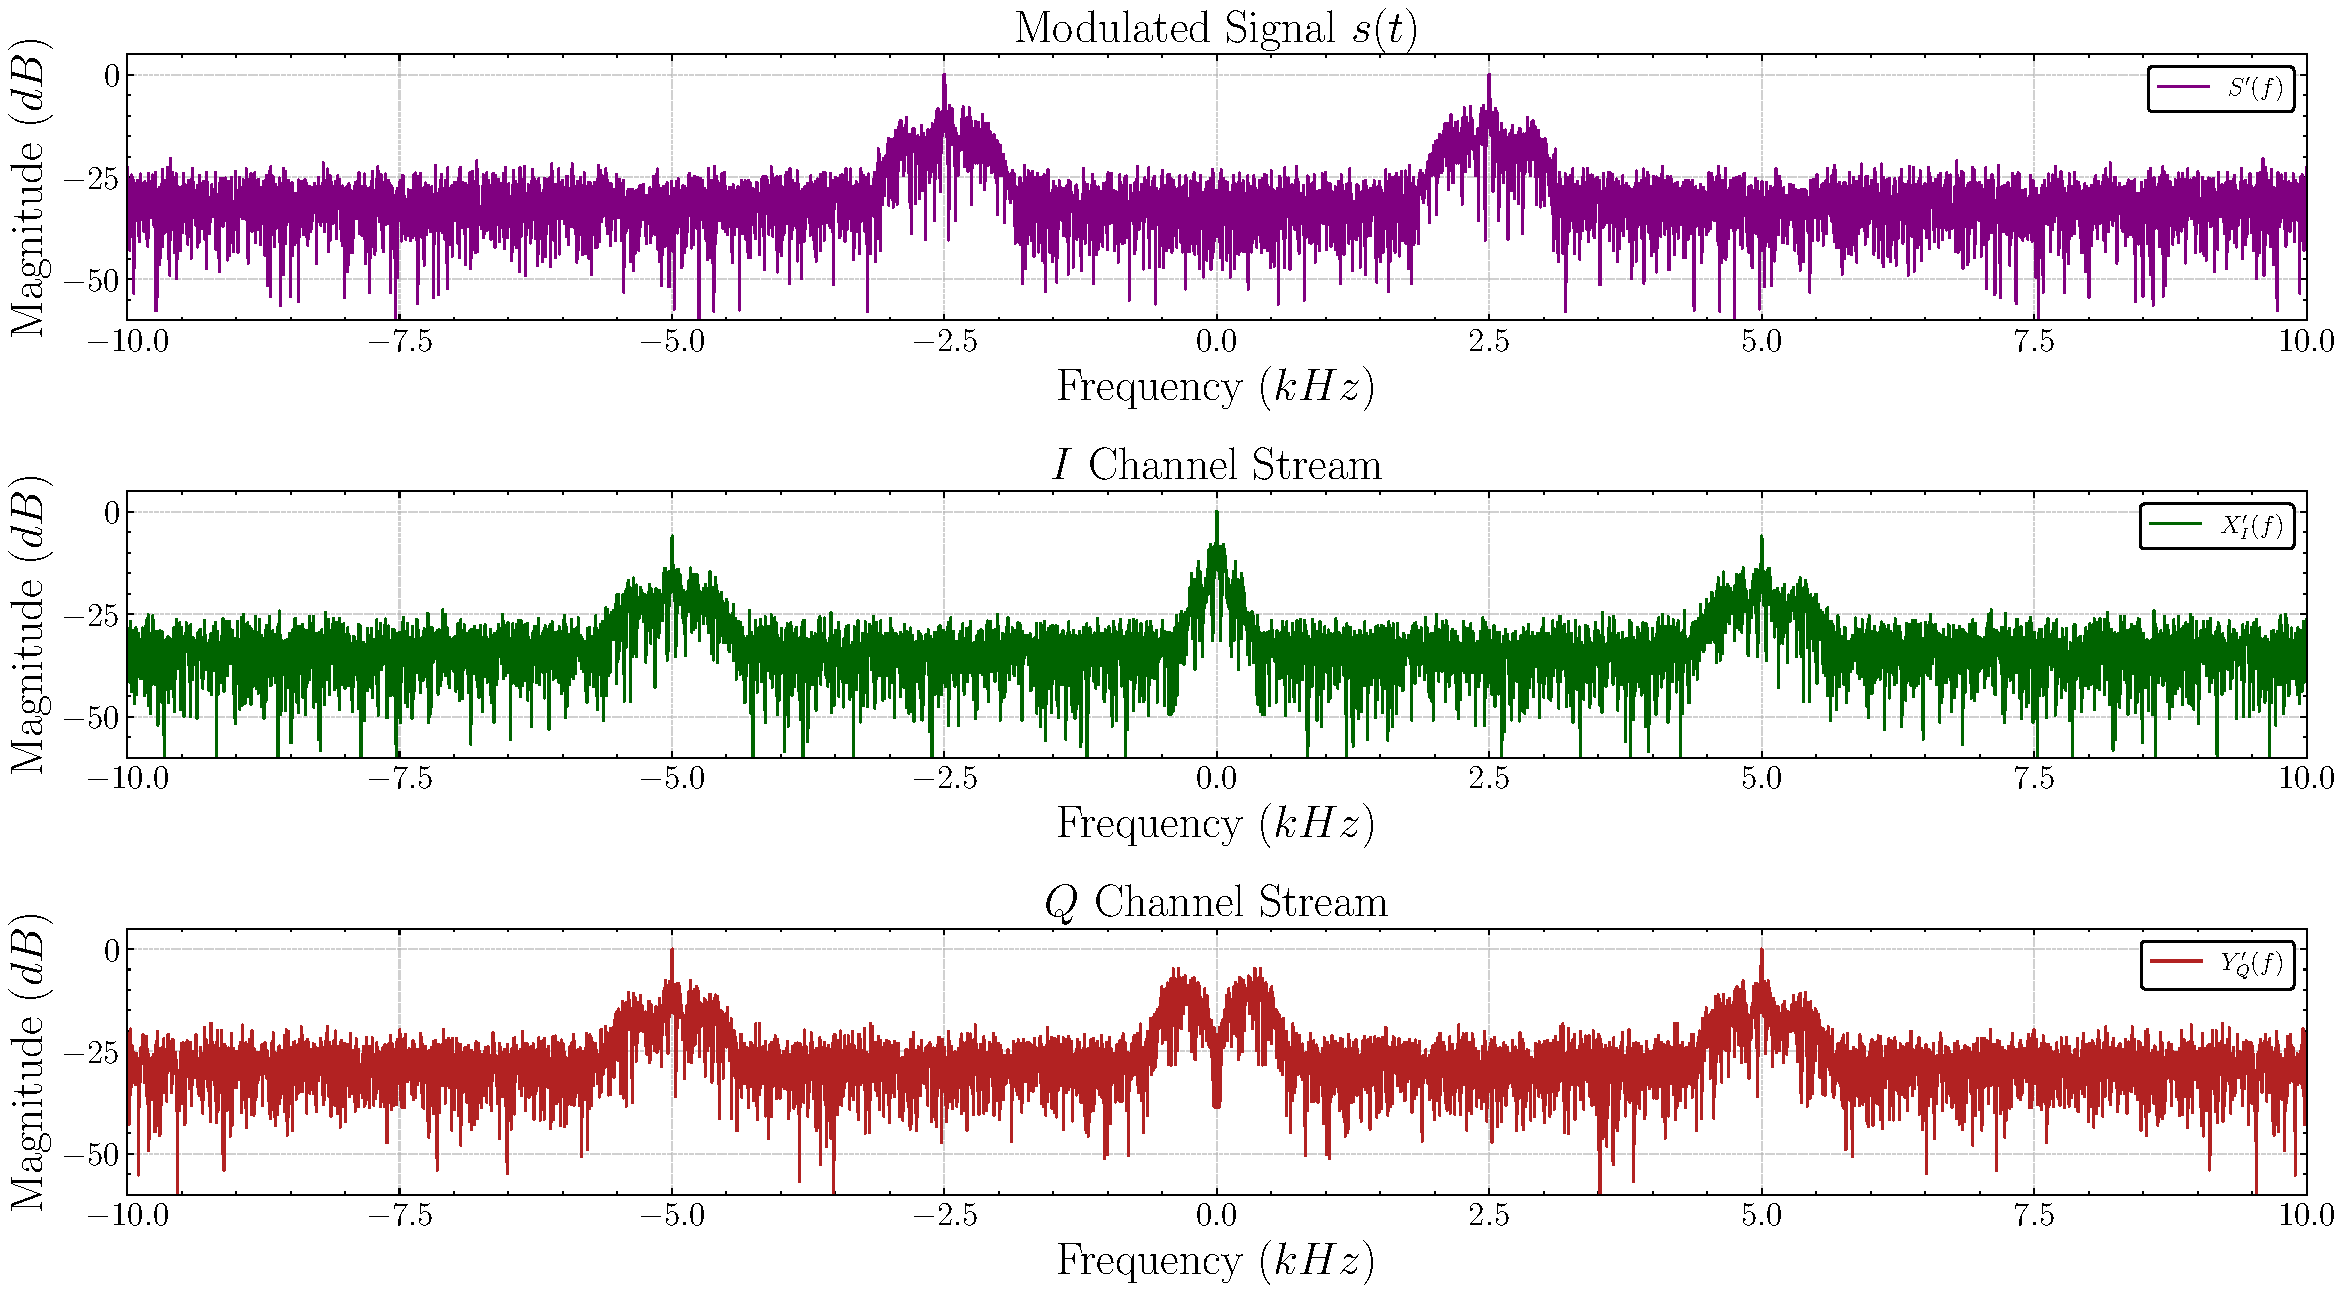
\includegraphics[width=\linewidth]{assets/cap3/receiver_demodulator_freq.pdf}
\end{figure}

\subsection{Filtragem}\label{sec:filtragem}

Após a demodulação, o próximo passo é a filtragem dos canais \gls{cI} e \gls{cQ} para remover as componentes de alta frequência geradas no processo de demodulação, bem como reduzir o máximo possível ruído presente em cada canal. A filtragem é realizada em duas etapas, primeiramente uma filtragem passa baixa para remover as componentes de alta frequência, conforme detalhado na seção \ref{sec:filtering}, resultando nos sinais \gls{dIprime} e \gls{dQprime}, conforme ilustrado na \autoref{fig:receiver_lpf}.

\begin{figure}[H]
	\centering
	\caption{Filtragem passa baixa dos canais $I$ e $Q$}\label{fig:receiver_lpf}
	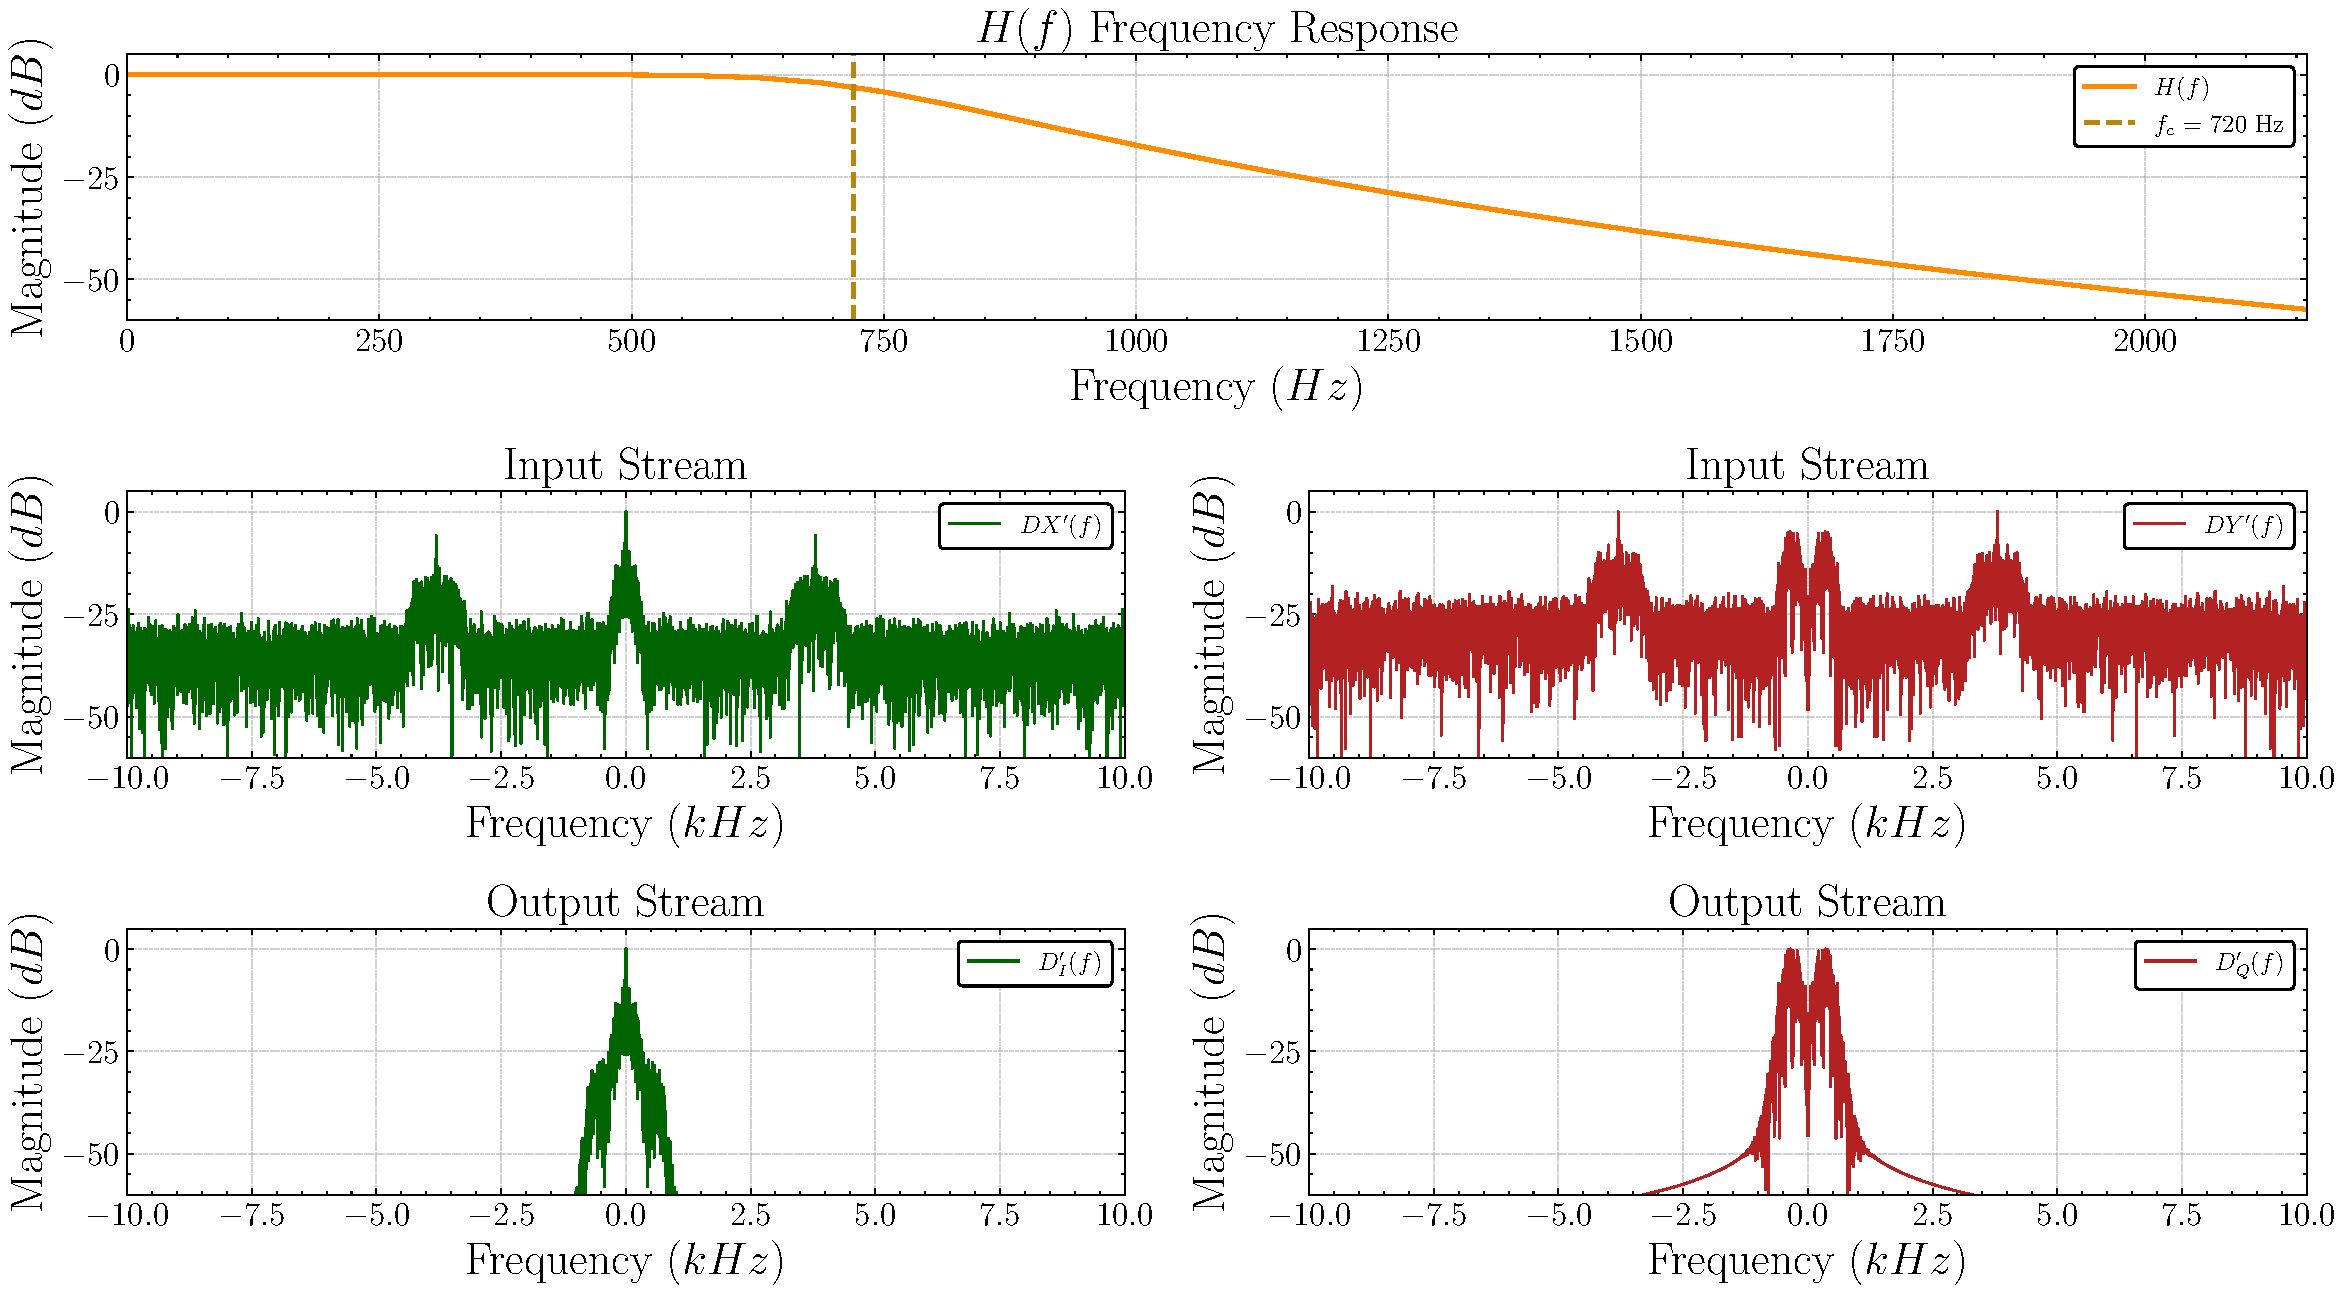
\includegraphics[width=\linewidth]{assets/cap3/receiver_lpf_freq.pdf}
\end{figure}

Em seguida, os sinais \gls{dIprime} e \gls{dQprime} já filtrados são submetidos outra filtragem, com o objetivo de maximizar a \gls{SNR} do sinal, para isso é aplicada uma filtragem casada utilizando os mesmos filtros de pulso utilizados na modulação de pulso porem invertidos no tempo, ou seja, com resposta ao impulso \gls{gti}, conforme detalhado na seção \ref{sec:filtering}, resultando nos sinais \gls{Iprime} e \gls{Qprime}. O processo de filtragem casada é ilustrado na \autoref{fig:receiver_matchedfilter}.

\begin{figure}[H]
	\centering
	\caption{Filtragem casada dos canais $I$ e $Q$}\label{fig:receiver_matchedfilter}
	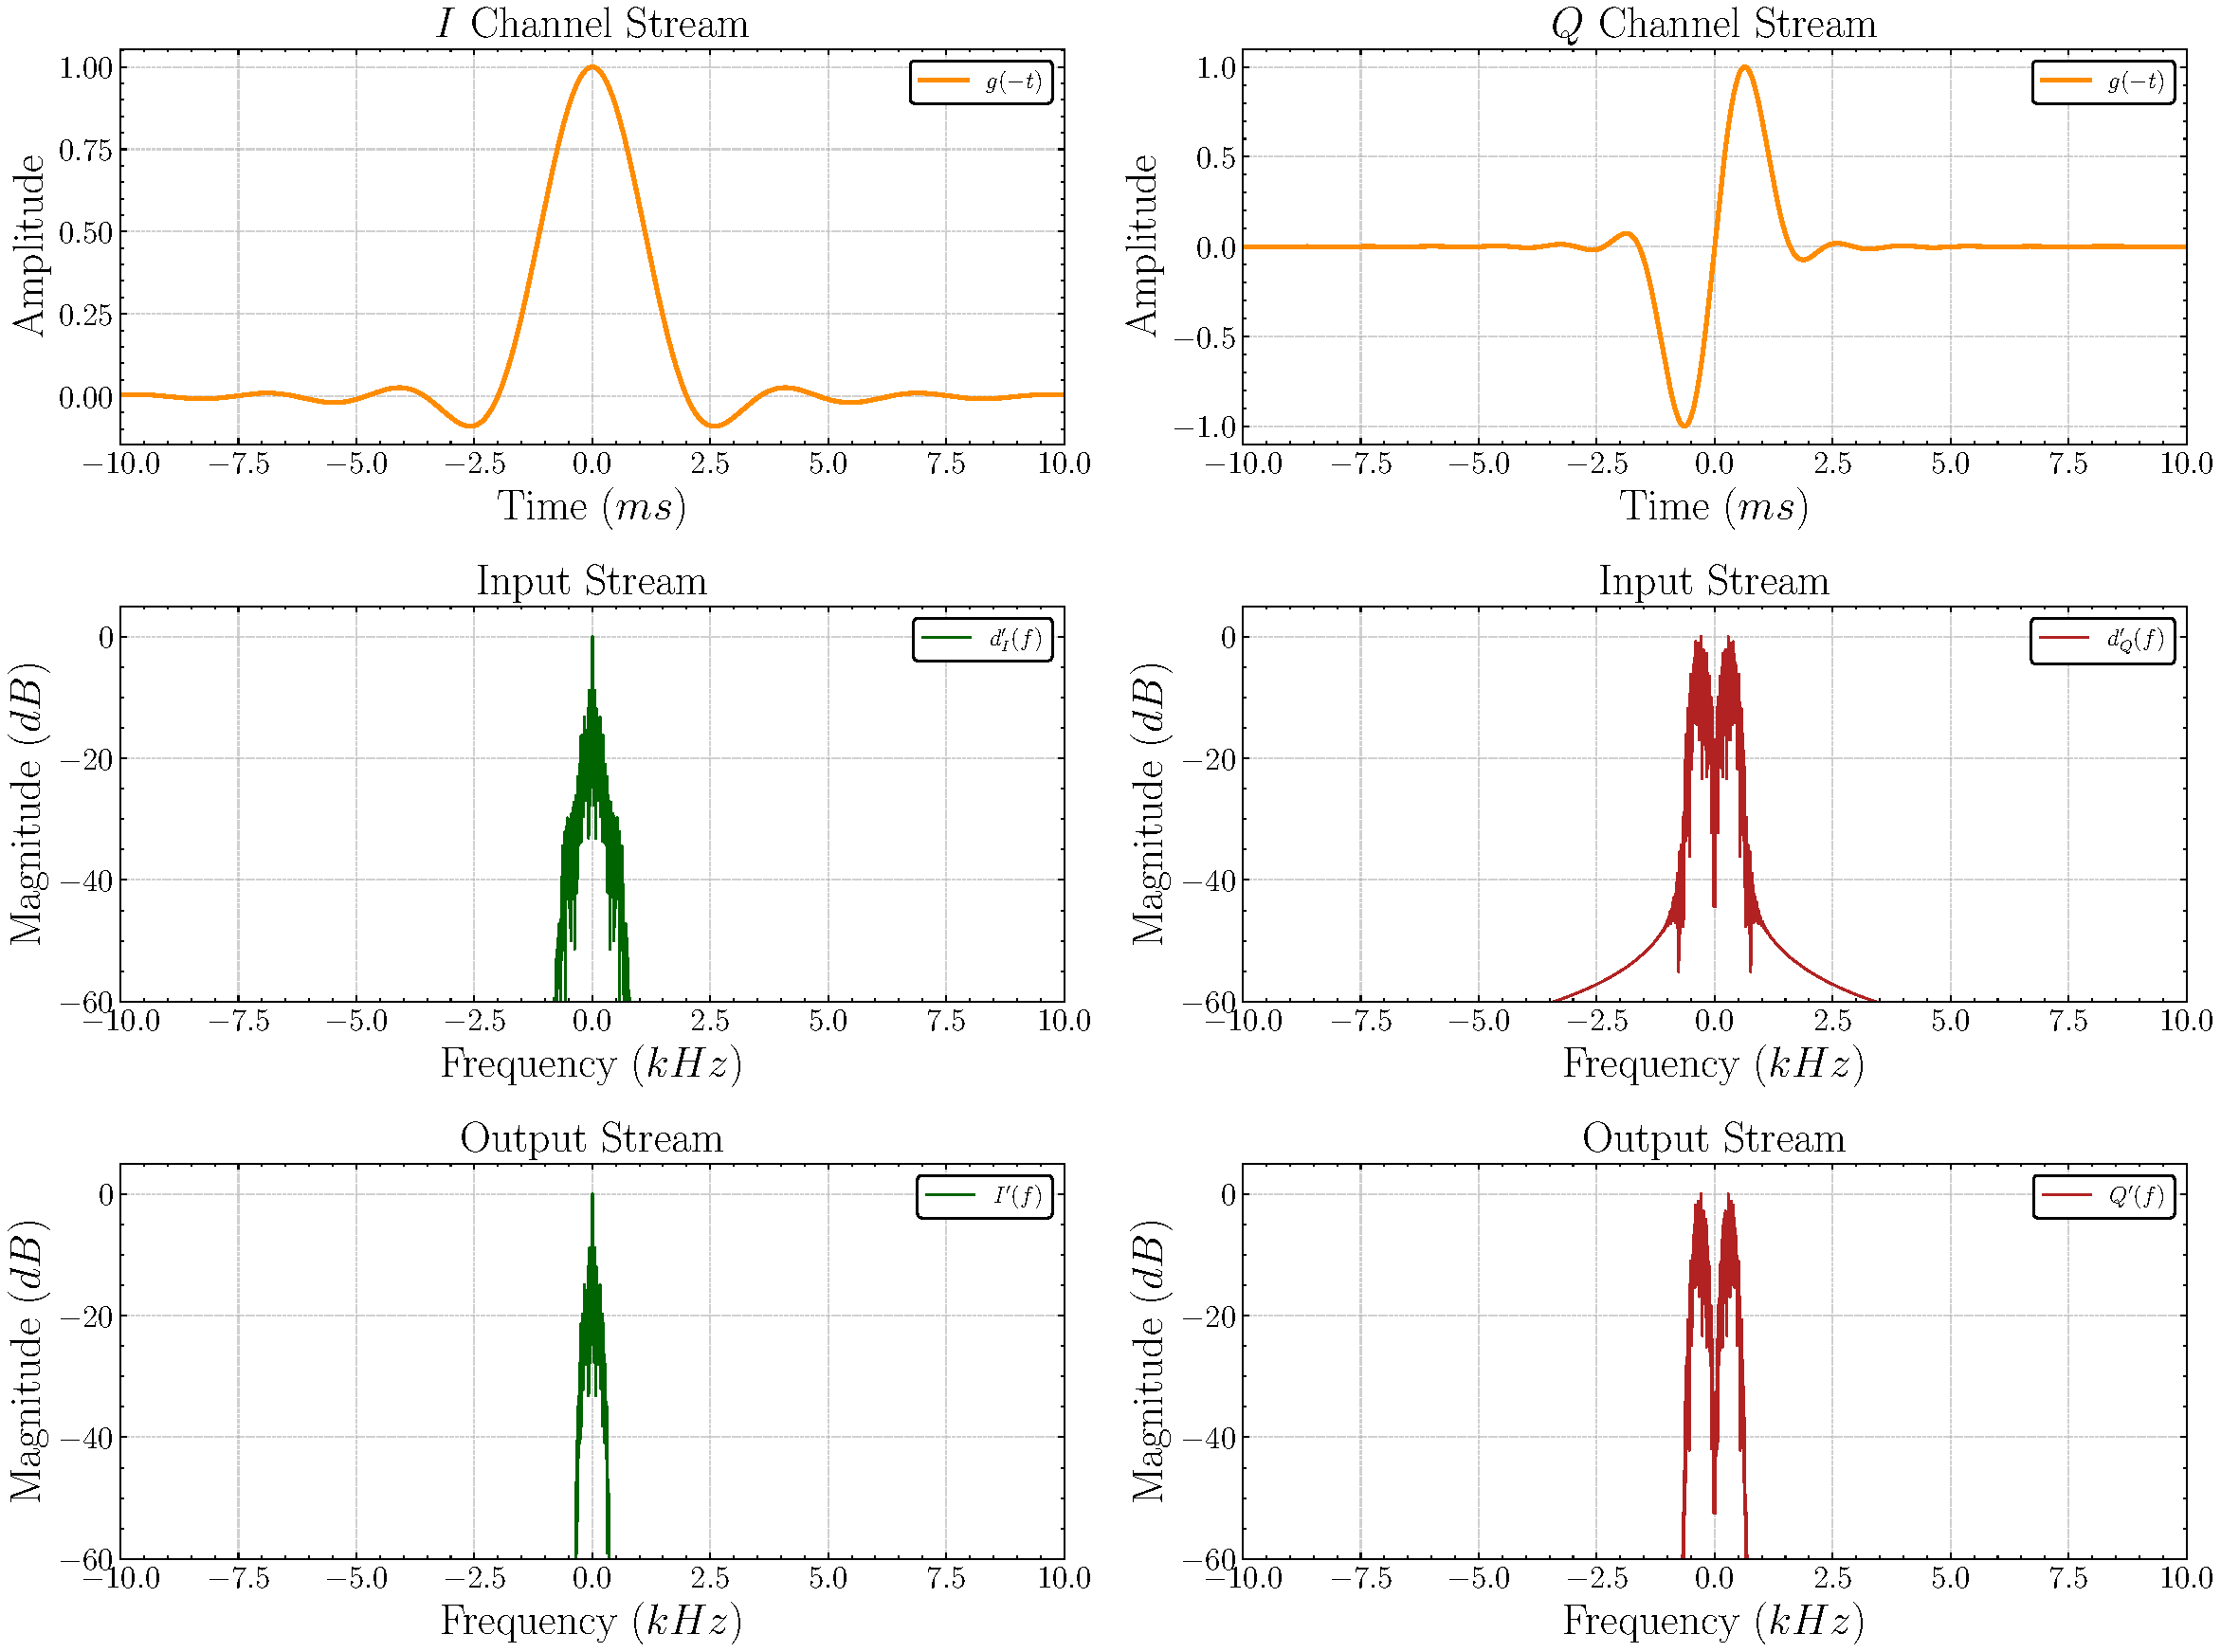
\includegraphics[width=\linewidth]{assets/cap3/receiver_mf_freq.pdf}
\end{figure}

Assim, os sinais \gls{Iprime} e \gls{Qprime} estão prontos para a sincronização de símbolos, conforme detalhado na seção \ref{sec:sincronizacao}.

\subsection{Sincronização de símbolos}\label{sec:sincronizacao}

Para poder recuperar os bits transmitidos, é necessário realizar a sincronização de símbolos para saber o delay inicial de amostragem \gls{tau}, e então utilizar esse valor para iniciar a amostragem com tempo de \gls{Tb} até o fim do sinal. Para a sincronização ocorrer, precisa-se iniciamente saber qual sequência esperar, e para isso deve-se montar o vetor de amostras esperadas para o sincronismo, esse processo é ilustrado na \autoref{fig:receiver_sync_diagram}.

\begin{figure}[H]
	\centering
	\caption{Diagrama de blocos para montagem do vetor de sincronismo}\label{fig:receiver_sync_diagram}
	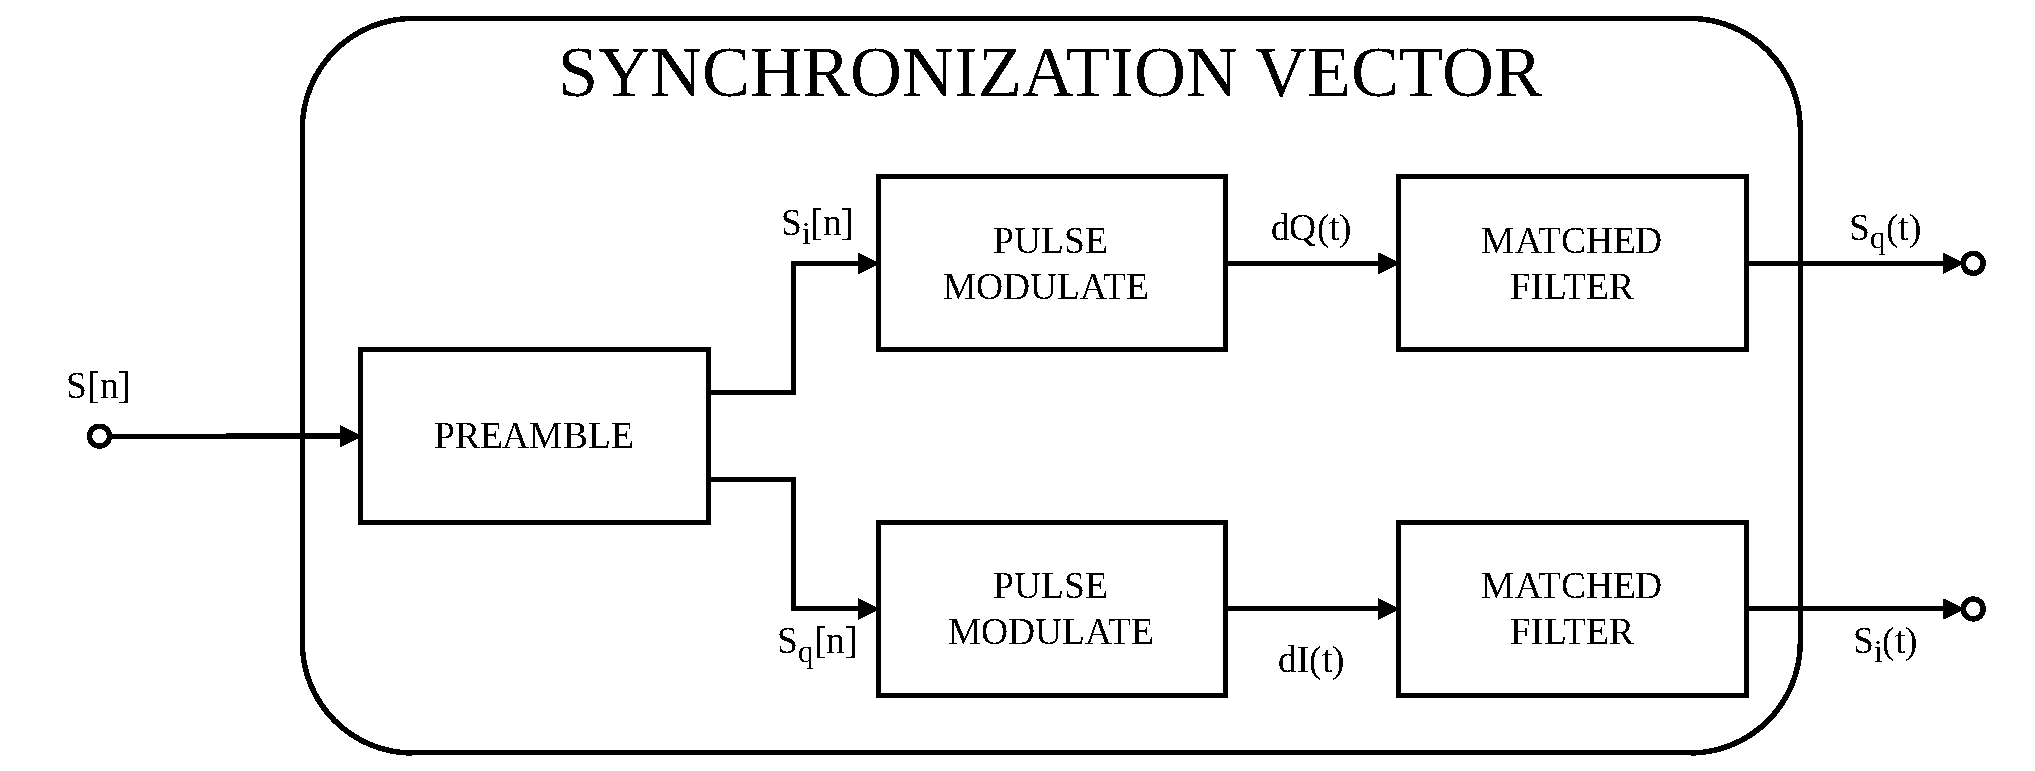
\includegraphics[width=\linewidth]{assets/diagrams/sync.pdf}
\end{figure}

Após a montagem do vetor de amostras esperadas para o sincronismo, que consiste em, gerar a sequência, superamostra-la, aplicar formatação de pulso nos canais \gls{cI} e \gls{cQ}, e em seguida filtragem casada, obtem-se o vetor de amostras esperadas para o sincronismo de cada canal, conforme ilustrado na \autoref{fig:receiver_sync_word}.

\begin{figure}[H]
	\centering
	\caption{Vetor de amostras esperadas para sincronismo com $I$ e $Q$}\label{fig:receiver_sync_word}
	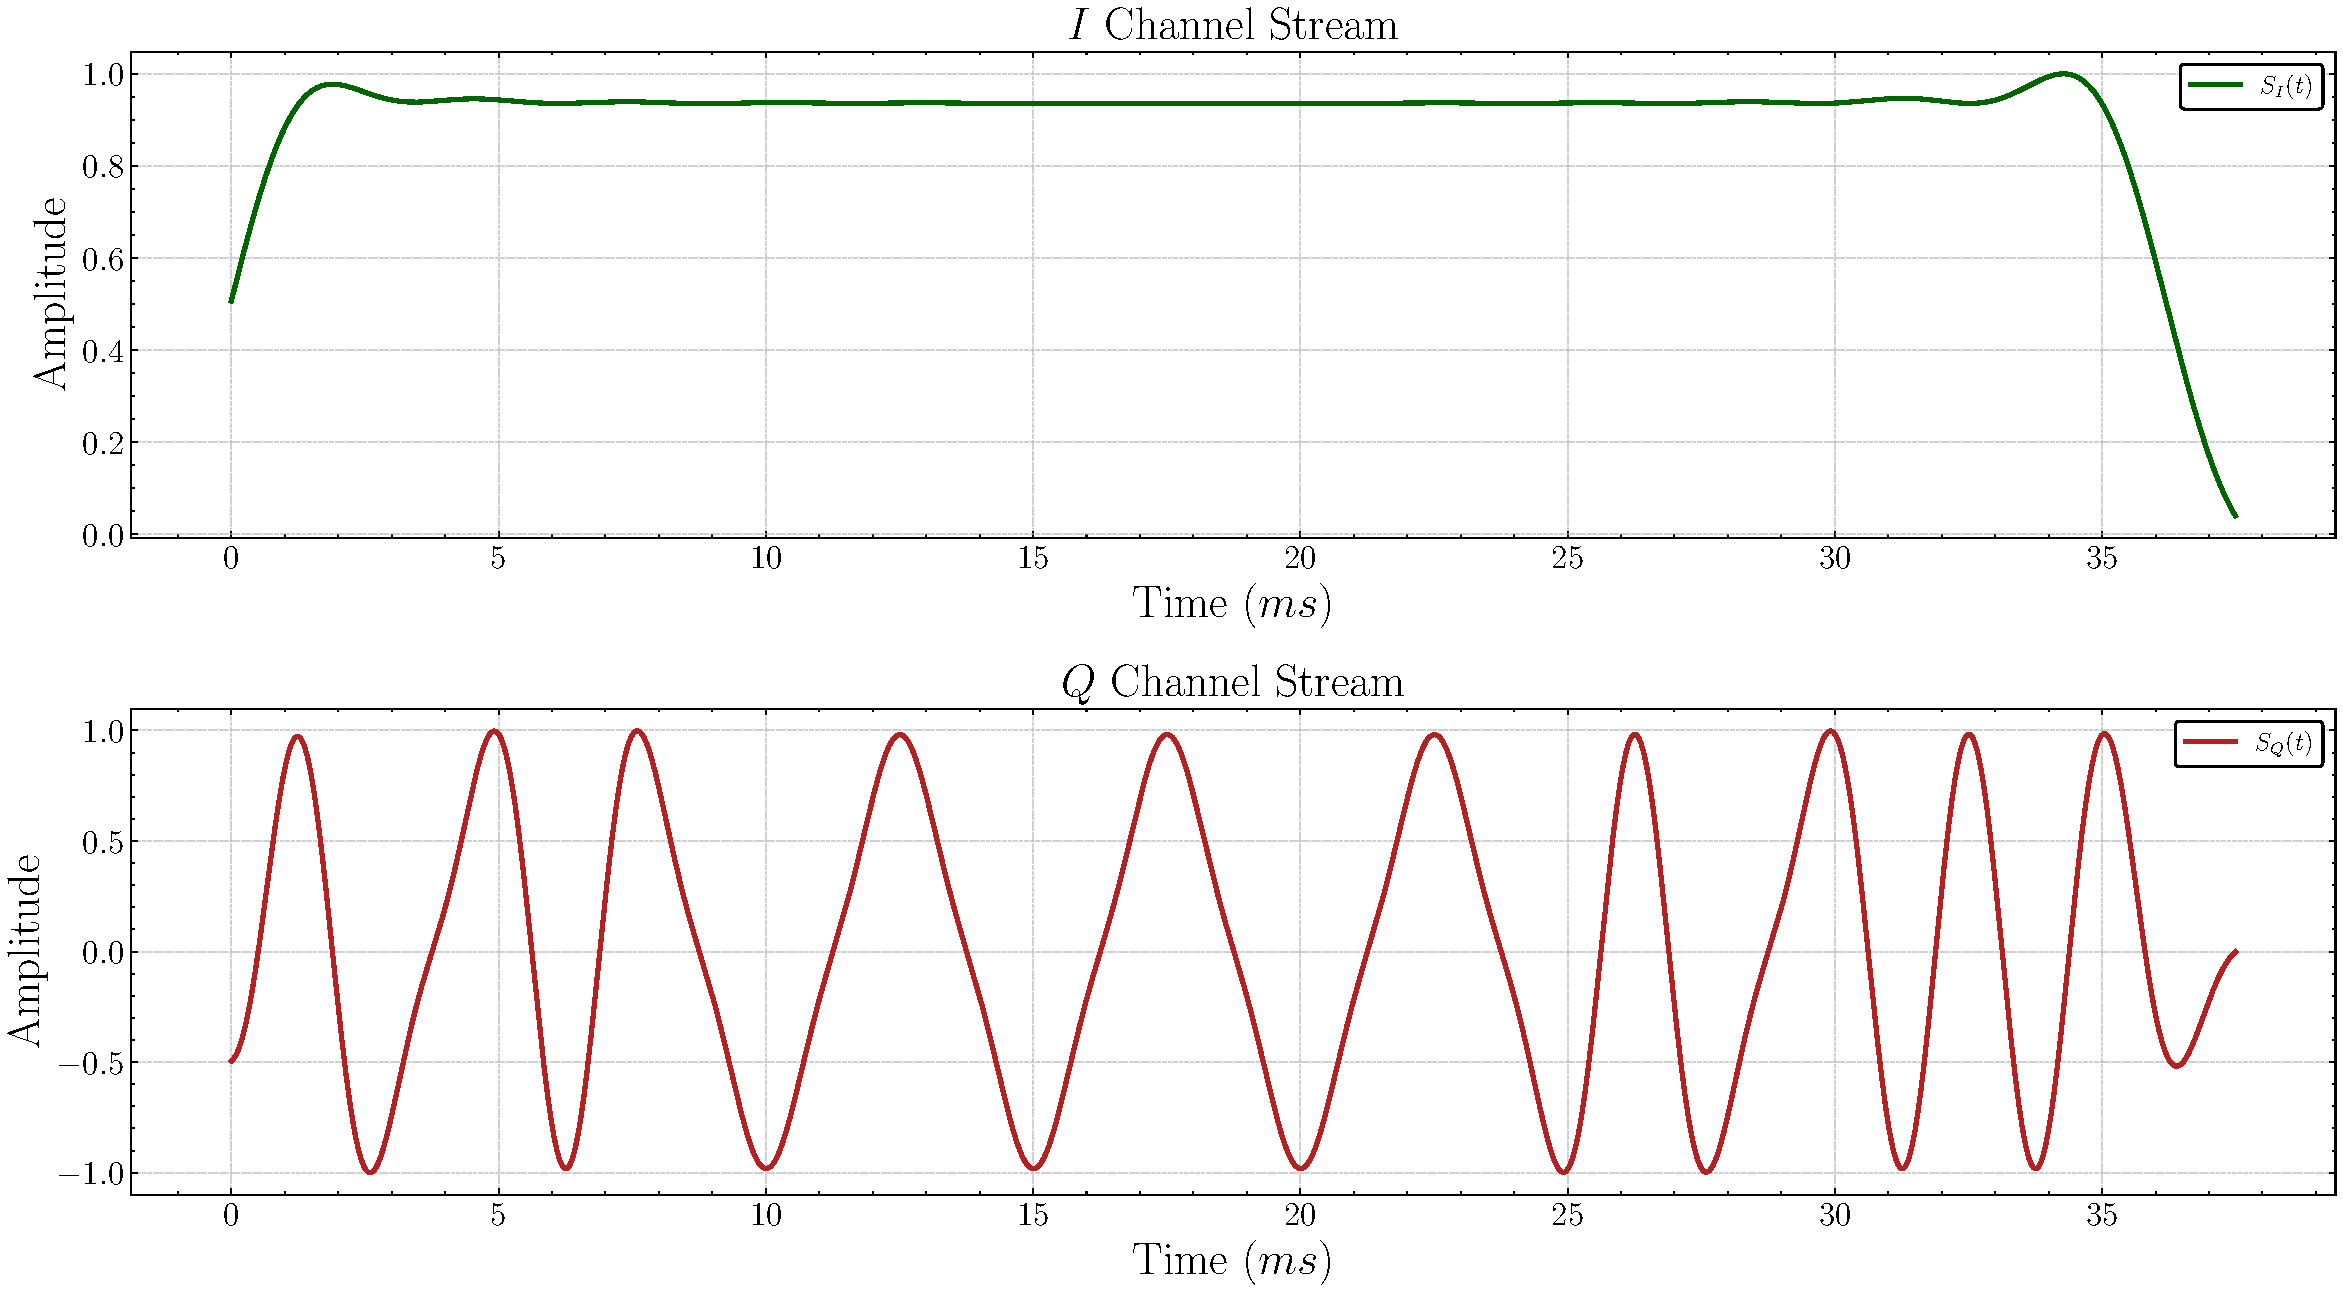
\includegraphics[width=\linewidth]{assets/cap3/example_synchronizer_word.pdf}
\end{figure}

Com o vetor de amostras esperadas para o sincronismo, é possível realizar a correlação, isto é, comparar o quanto se parece uma seção dos canais \gls{cI} e \gls{cQ} com o vetor de sincronismo, resultando no módulo de correlação, onde o pico máximo do módulo de correlação \gls{kmax} indica o ponto de início da transmissão. O processo de correlação para encontrar a amostra de máxima correlação é ilustrado nas \autoref{fig:receiver_corr} e \autoref{fig:receiver_sync}.

\begin{figure}[H]
	\centering
	\caption{Módulo de correlação entre $I$ e $Q$ e vetor de sincronismo}\label{fig:receiver_corr}
	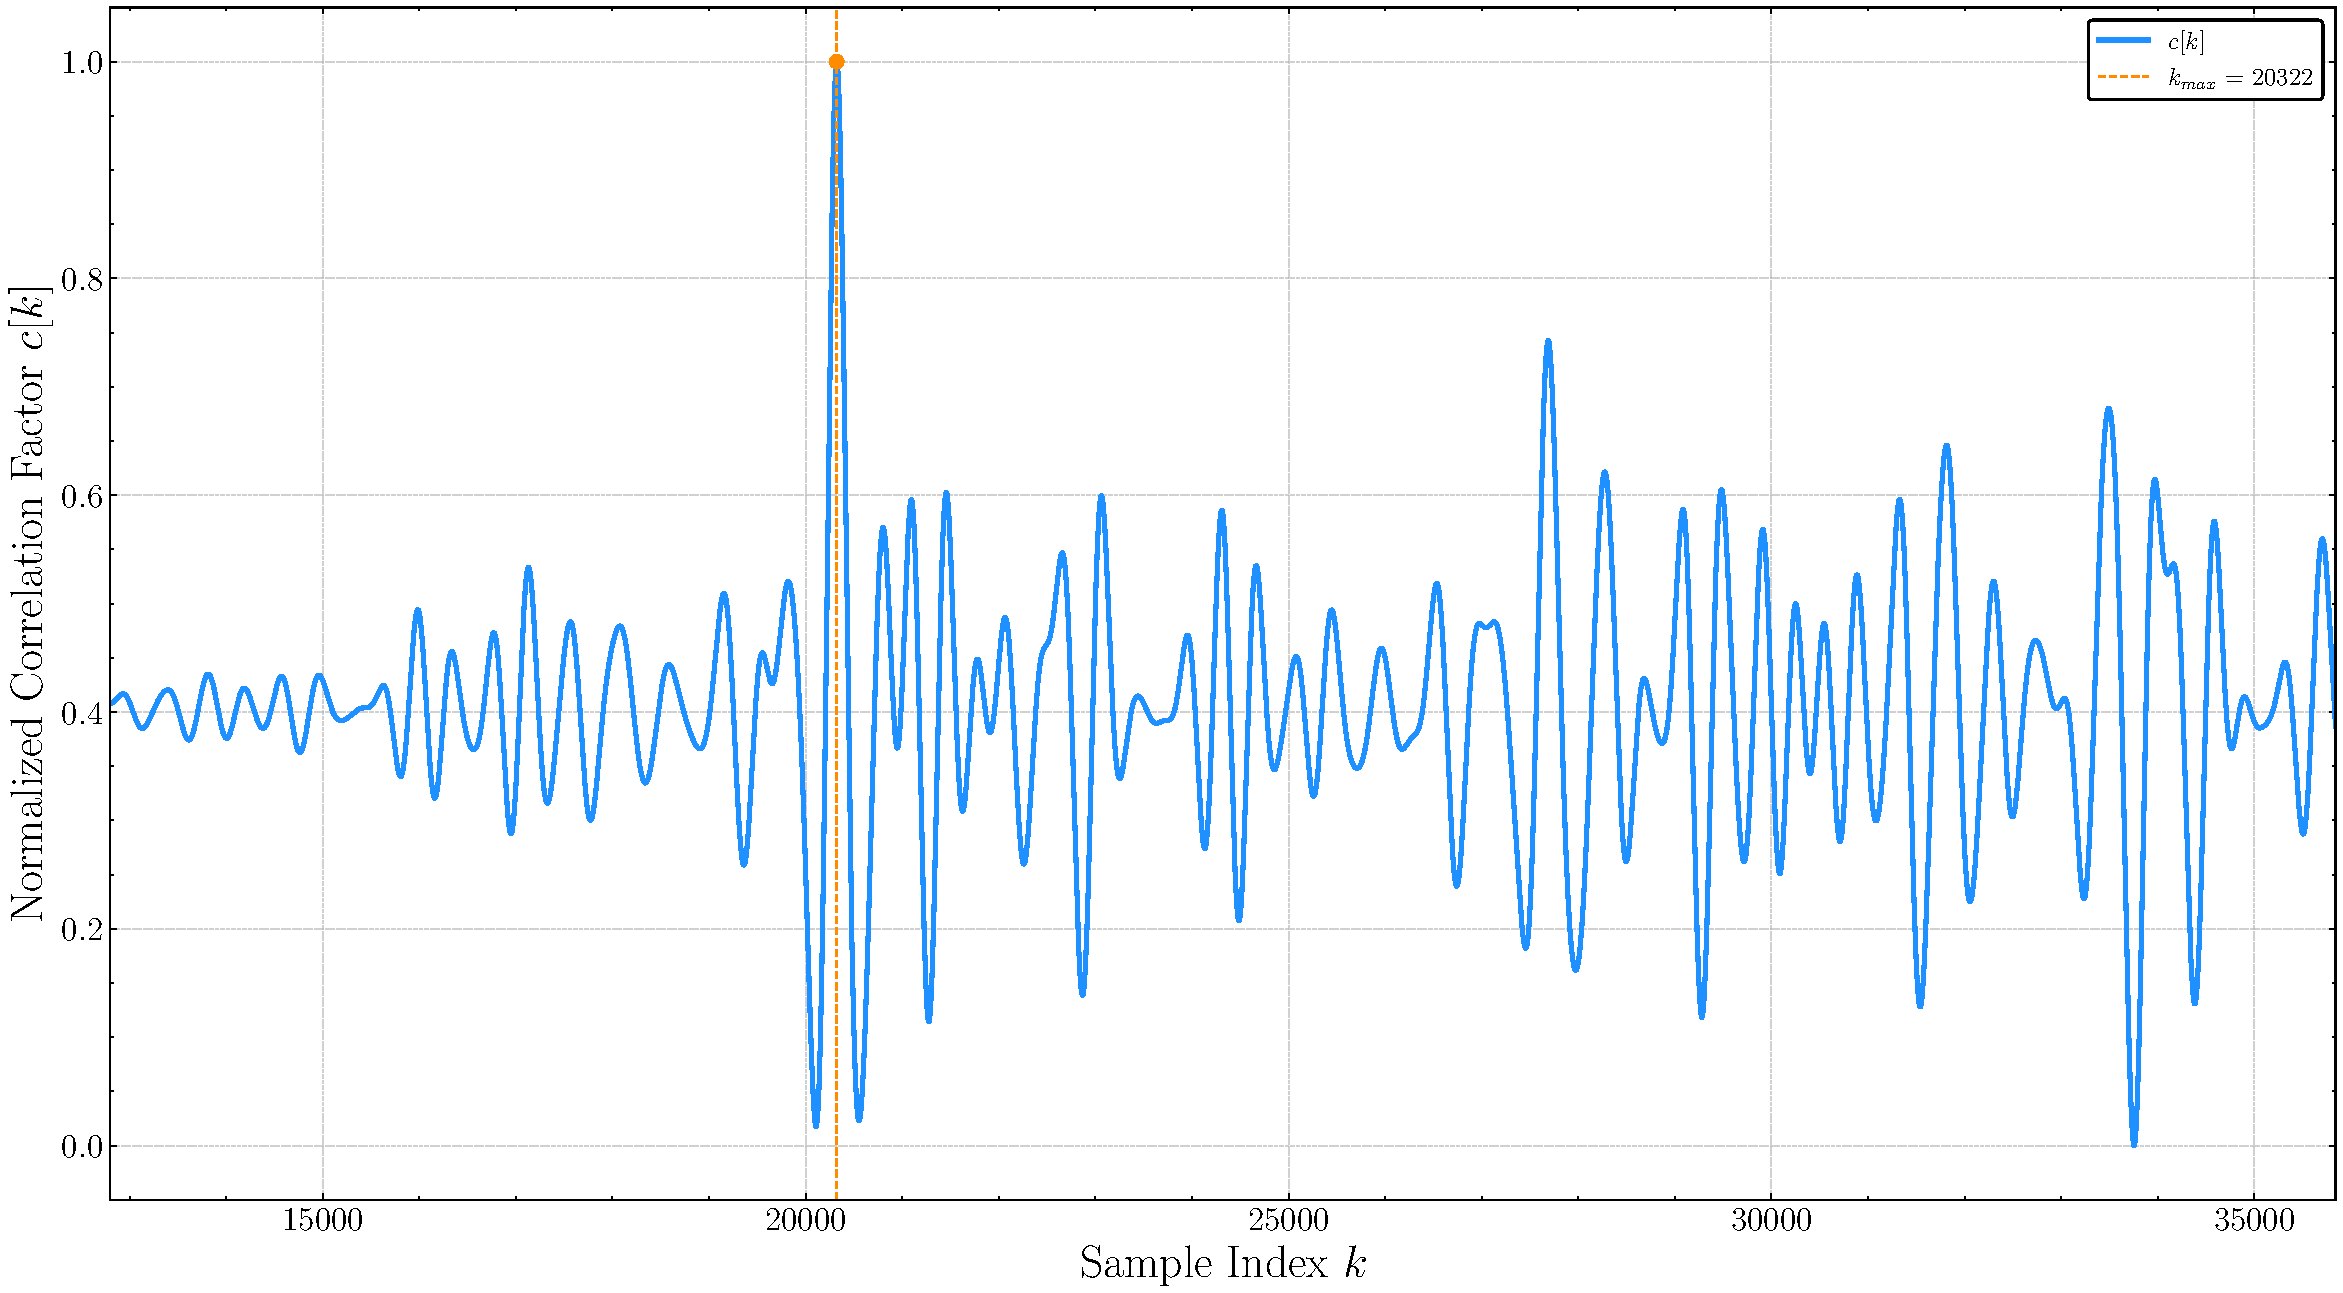
\includegraphics[width=\linewidth]{assets/cap3/receiver_sync_corr.pdf}
\end{figure}

Uma vez com o fator máximo de correlação, podemos facilmente determinar o delay inicial de amostragem como $\tau = f_s / k_{\text{max}}$, visto que a \gls{fs} é conhecida. Com o valor de \gls{tau} determinado, os canais \gls{cI} e \gls{cQ} estão prontos para serem amostrados a cada \gls{Tb} a partir do ponto inicial \gls{tau}. O processo de sincronização de símbolos é ilustrado na \autoref{fig:receiver_sync}.

\begin{figure}[H]
	\centering
	\caption{Sicronização de $I$ e $Q$ com vetor de sincronismo}\label{fig:receiver_sync}
	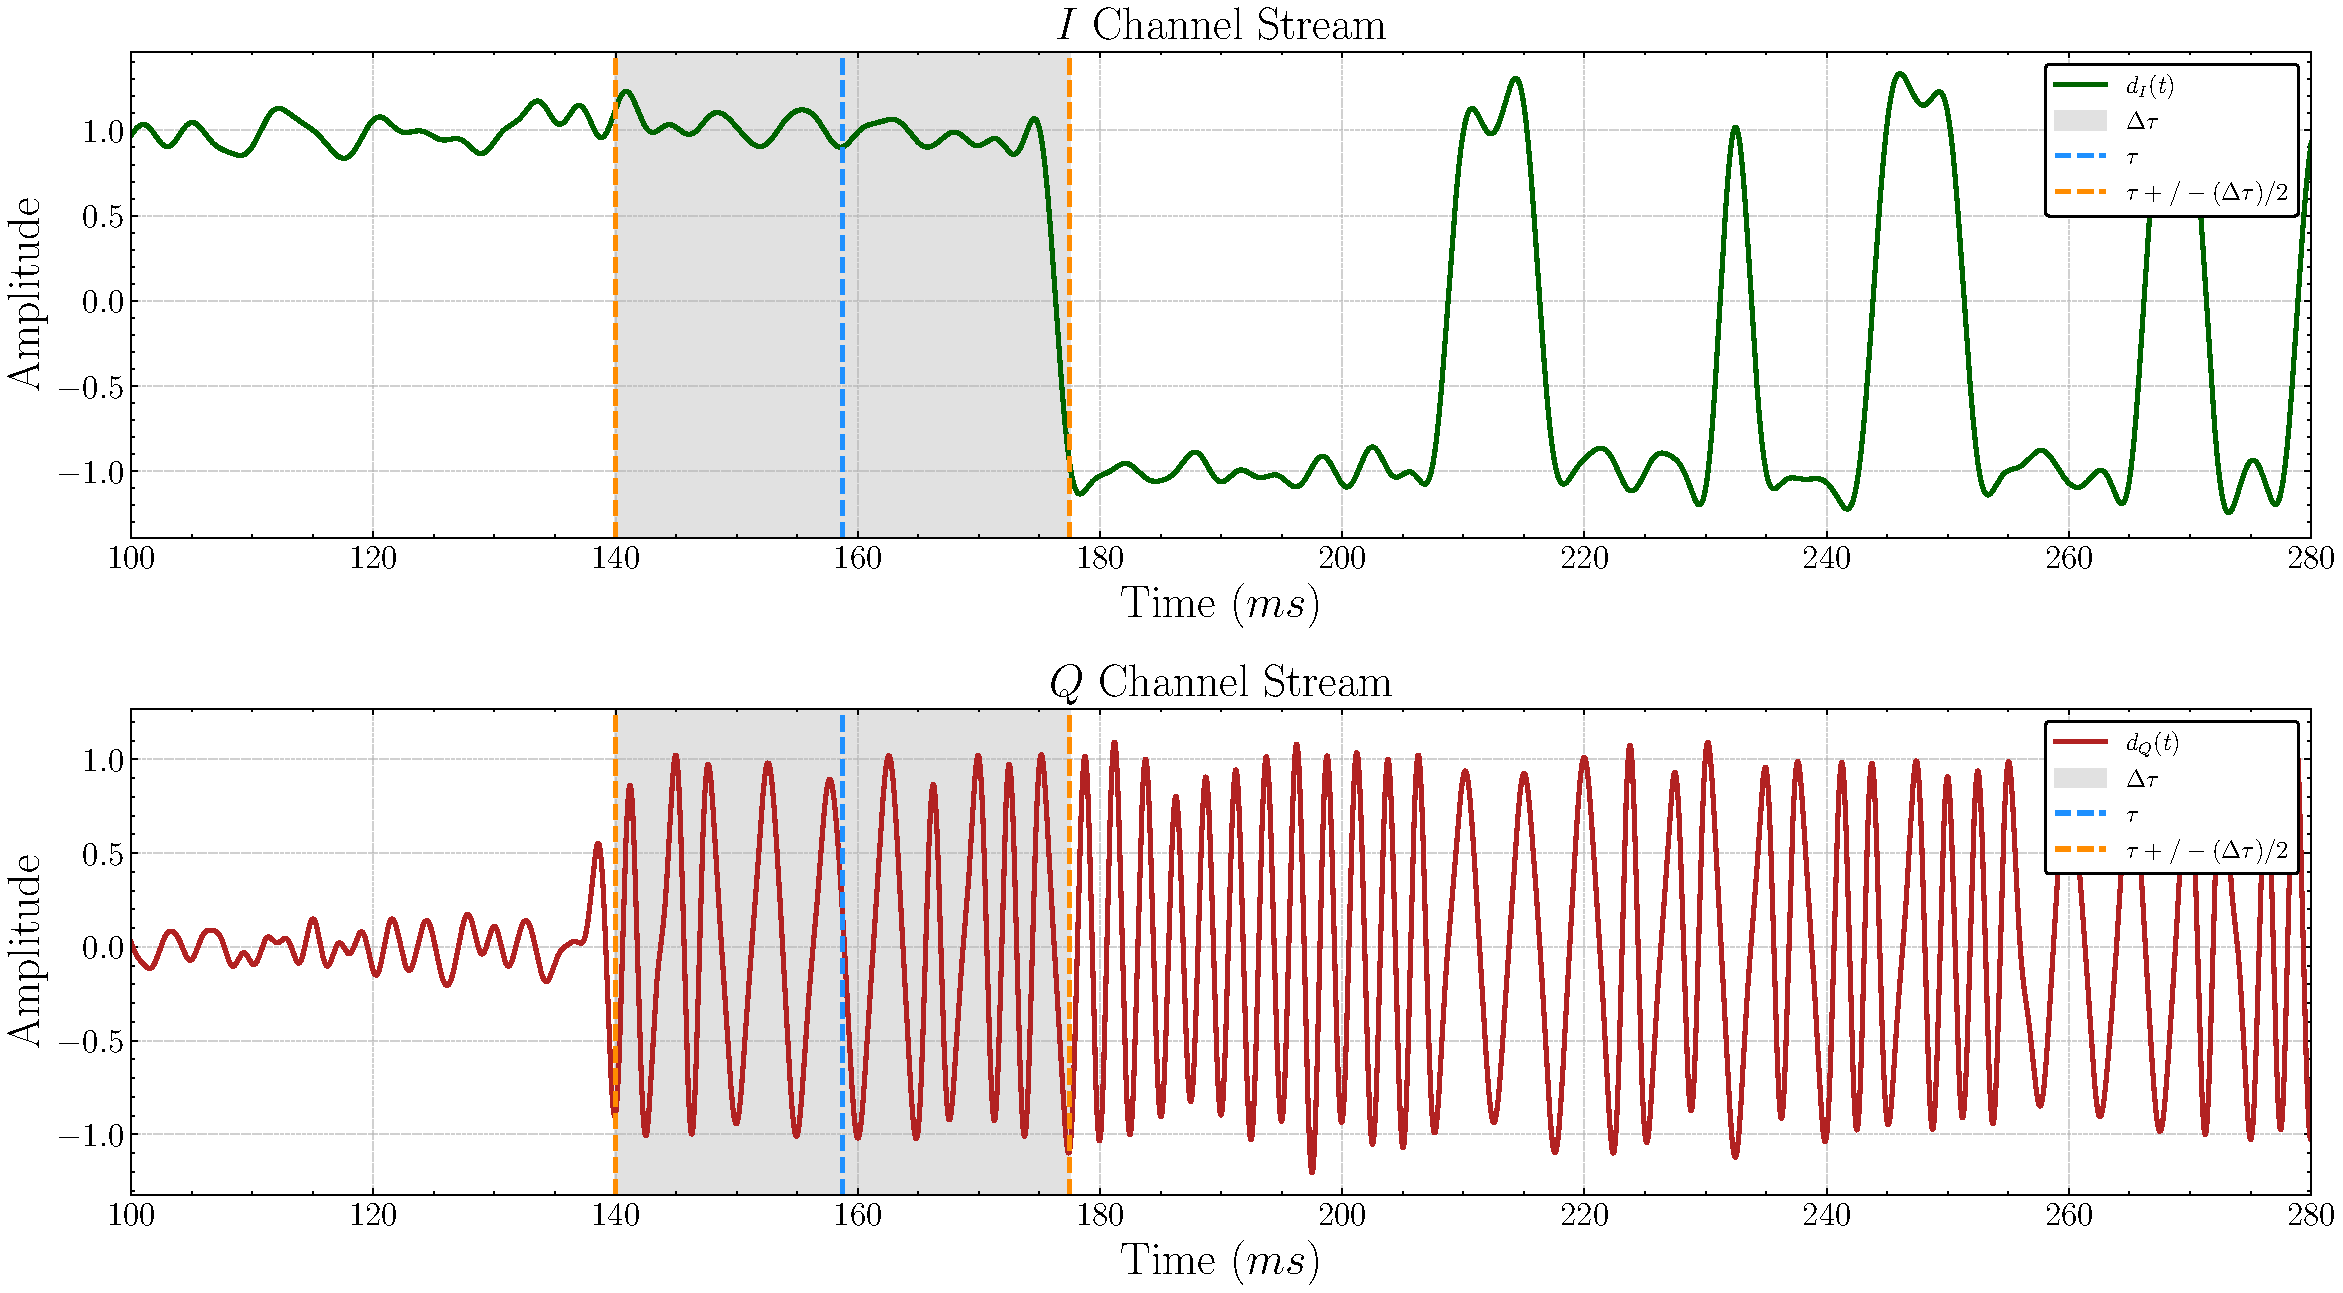
\includegraphics[width=\linewidth]{assets/cap3/receiver_sync_time.pdf}
\end{figure}

Na \autoref{fig:receiver_sync} a região em cinza representa o período de preâmbulo, onde é possível observar que o pico máximo de correlação ocorre exatamente na metade do preâmbulo, ou seja, deve-se iniciar a amostragem a partir de $\tau + (\Delta \tau)/2$, onde $\Delta \tau$ é o comprimento do preâmbulo em amostras ($\Delta \tau = \text{\gls{Lsync}} \cdot f_s/R_b$). 

\subsection{Decisão de símbolos}\label{sec:decisao_simbolos}

Com o valor de \gls{tau} determinado, os canais \gls{cI} e \gls{cQ} estão prontos para serem amostrados a cada \gls{Tb} a partir do ponto inicial \gls{tau}, resultando nos vetores de amostras \gls{Inprime} e \gls{Qnprime}. A decisão de símbolos é realizada através da comparação das amostras com um limiar definido, onde valores positivos são interpretados como $`1`$ e valores negativos como $`0`$. O processo de amostragem e decisão de símbolos é ilustrado nas \autoref{fig:receiver_sampler} e \autoref{fig:receiver_const}.

\begin{figure}[H]
	\centering
	\caption{Amostragem dos canais $I$ e $Q$ em $T_b$ a partir de \gls{tau}}\label{fig:receiver_sampler}
	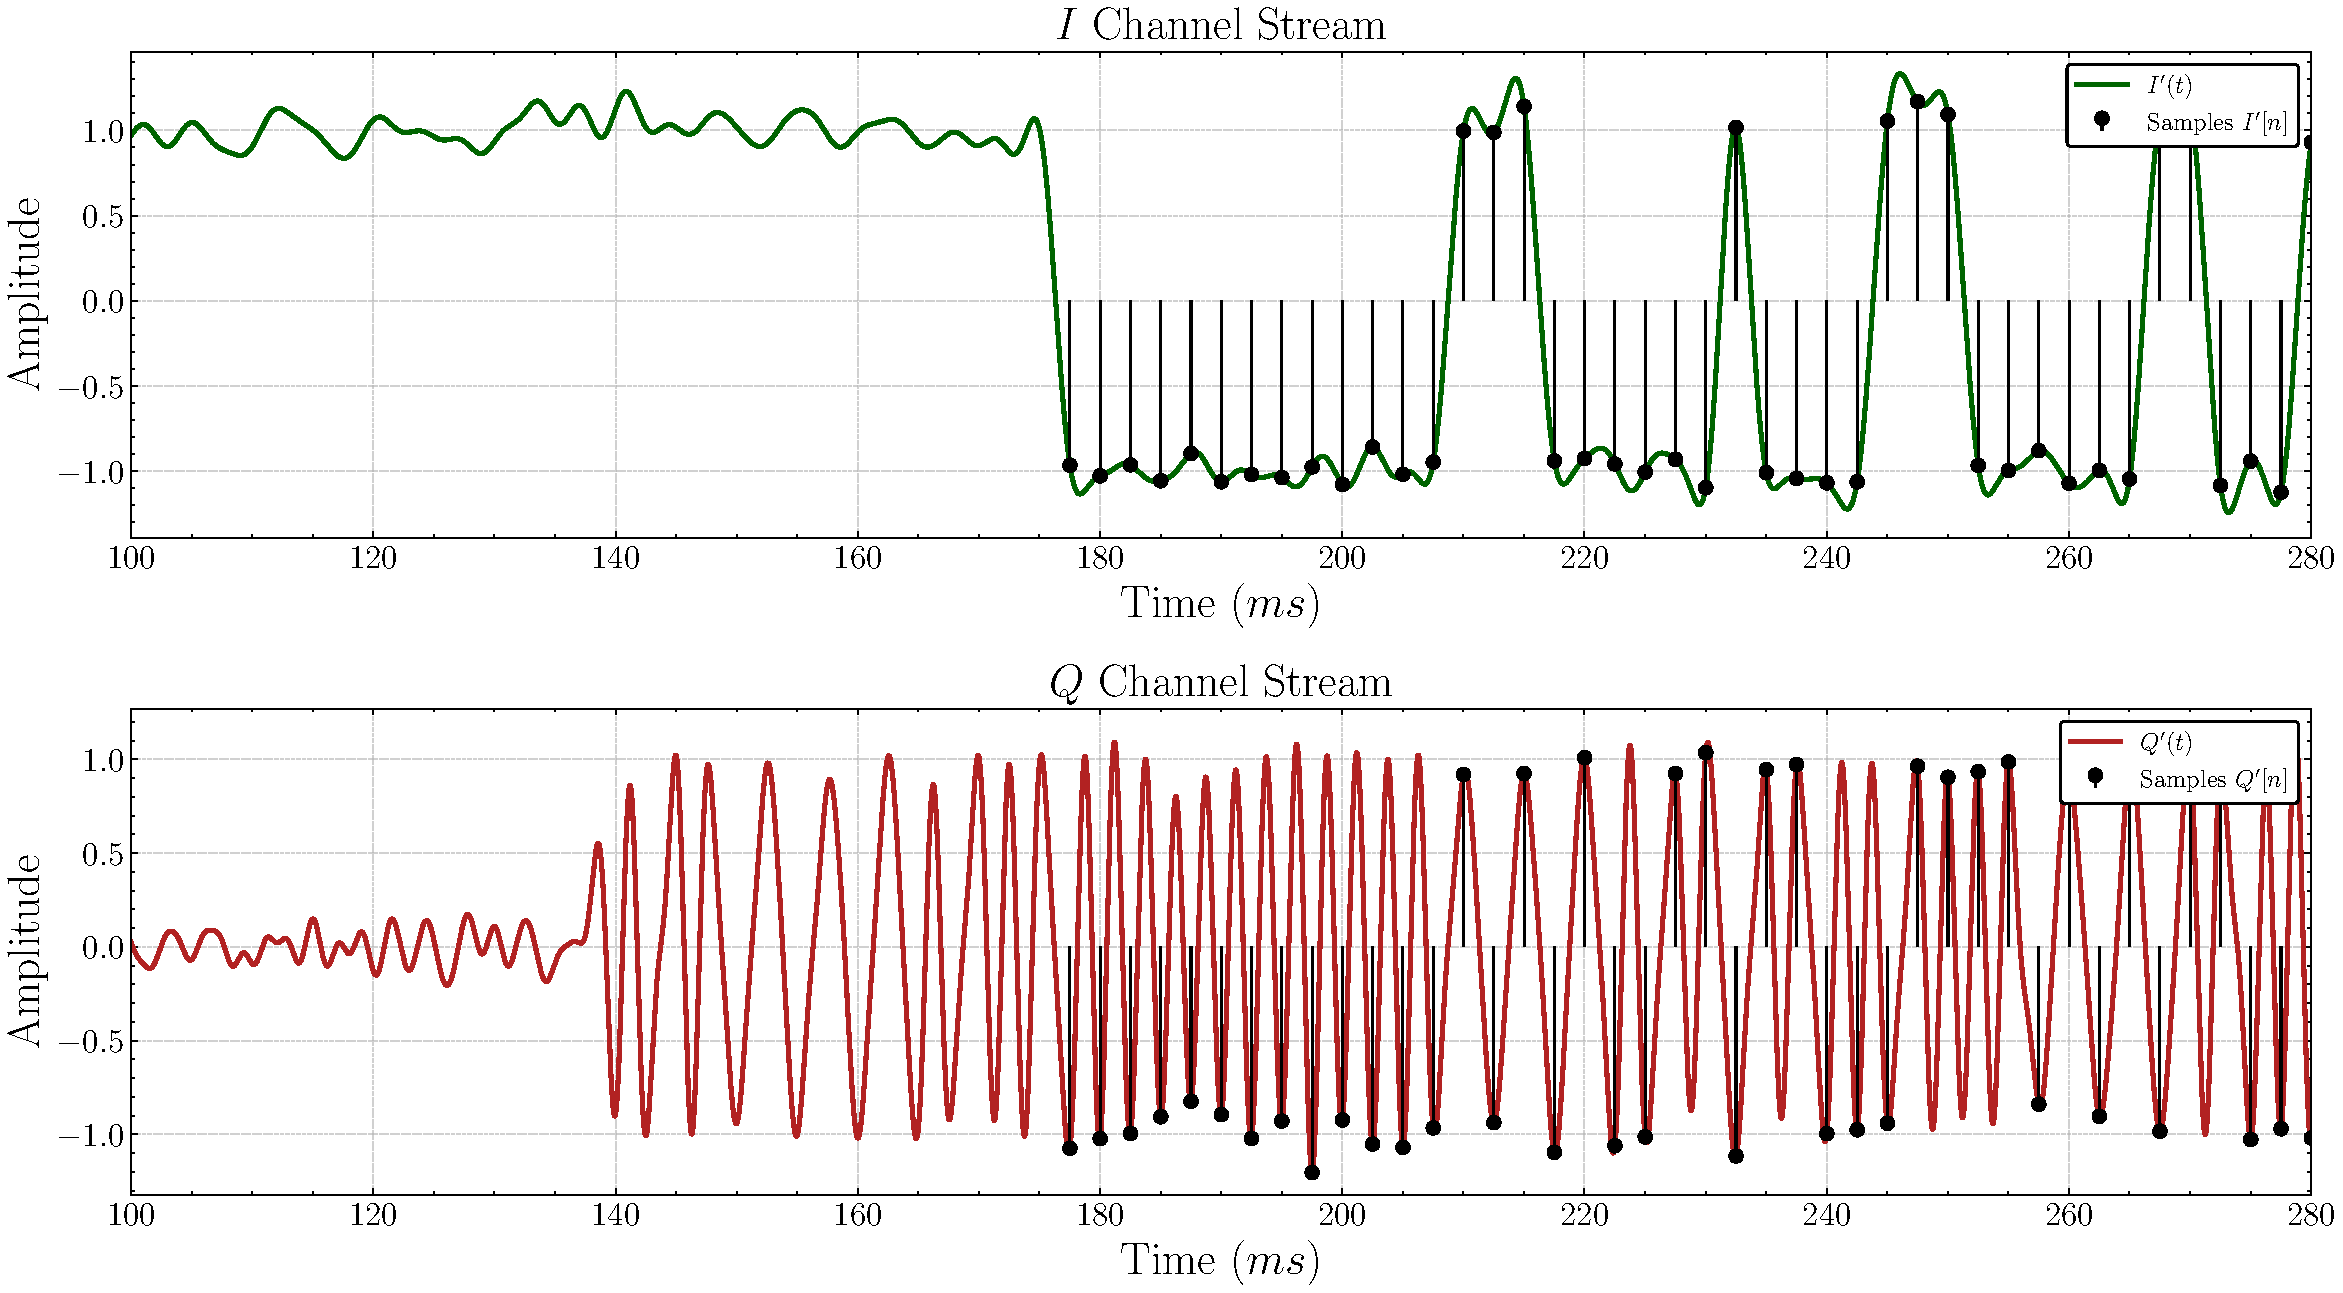
\includegraphics[width=\linewidth]{assets/cap3/receiver_sampler_time.pdf}
\end{figure}

Tendo os sinais \gls{dIprime} e \gls{dQprime} e seus correspondentes vetores de amostras \gls{Inprime} e \gls{Qnprime}, é possível observar a constelação dos canais \gls{cI} e \gls{cQ} no \gls{iqplane}, antes e após a amostragem, conforme ilustrado na \autoref{fig:receiver_const}, nota-se que na direita da imagem, a constelação é plotada de maneira contínua, ou seja, cada ponto representa um instante de tempo \gls{t}, enquanto que na esquerda da imagem, a constelação é plotada apenas com os pontos amostrados, ou seja, cada ponto representa um símbolo sobre o tempo \gls{Tb}. 

\begin{figure}[H]
	\centering
	\caption{Constelação dos canais $I$ e $Q$ filtrados e amostrados}\label{fig:receiver_const}
	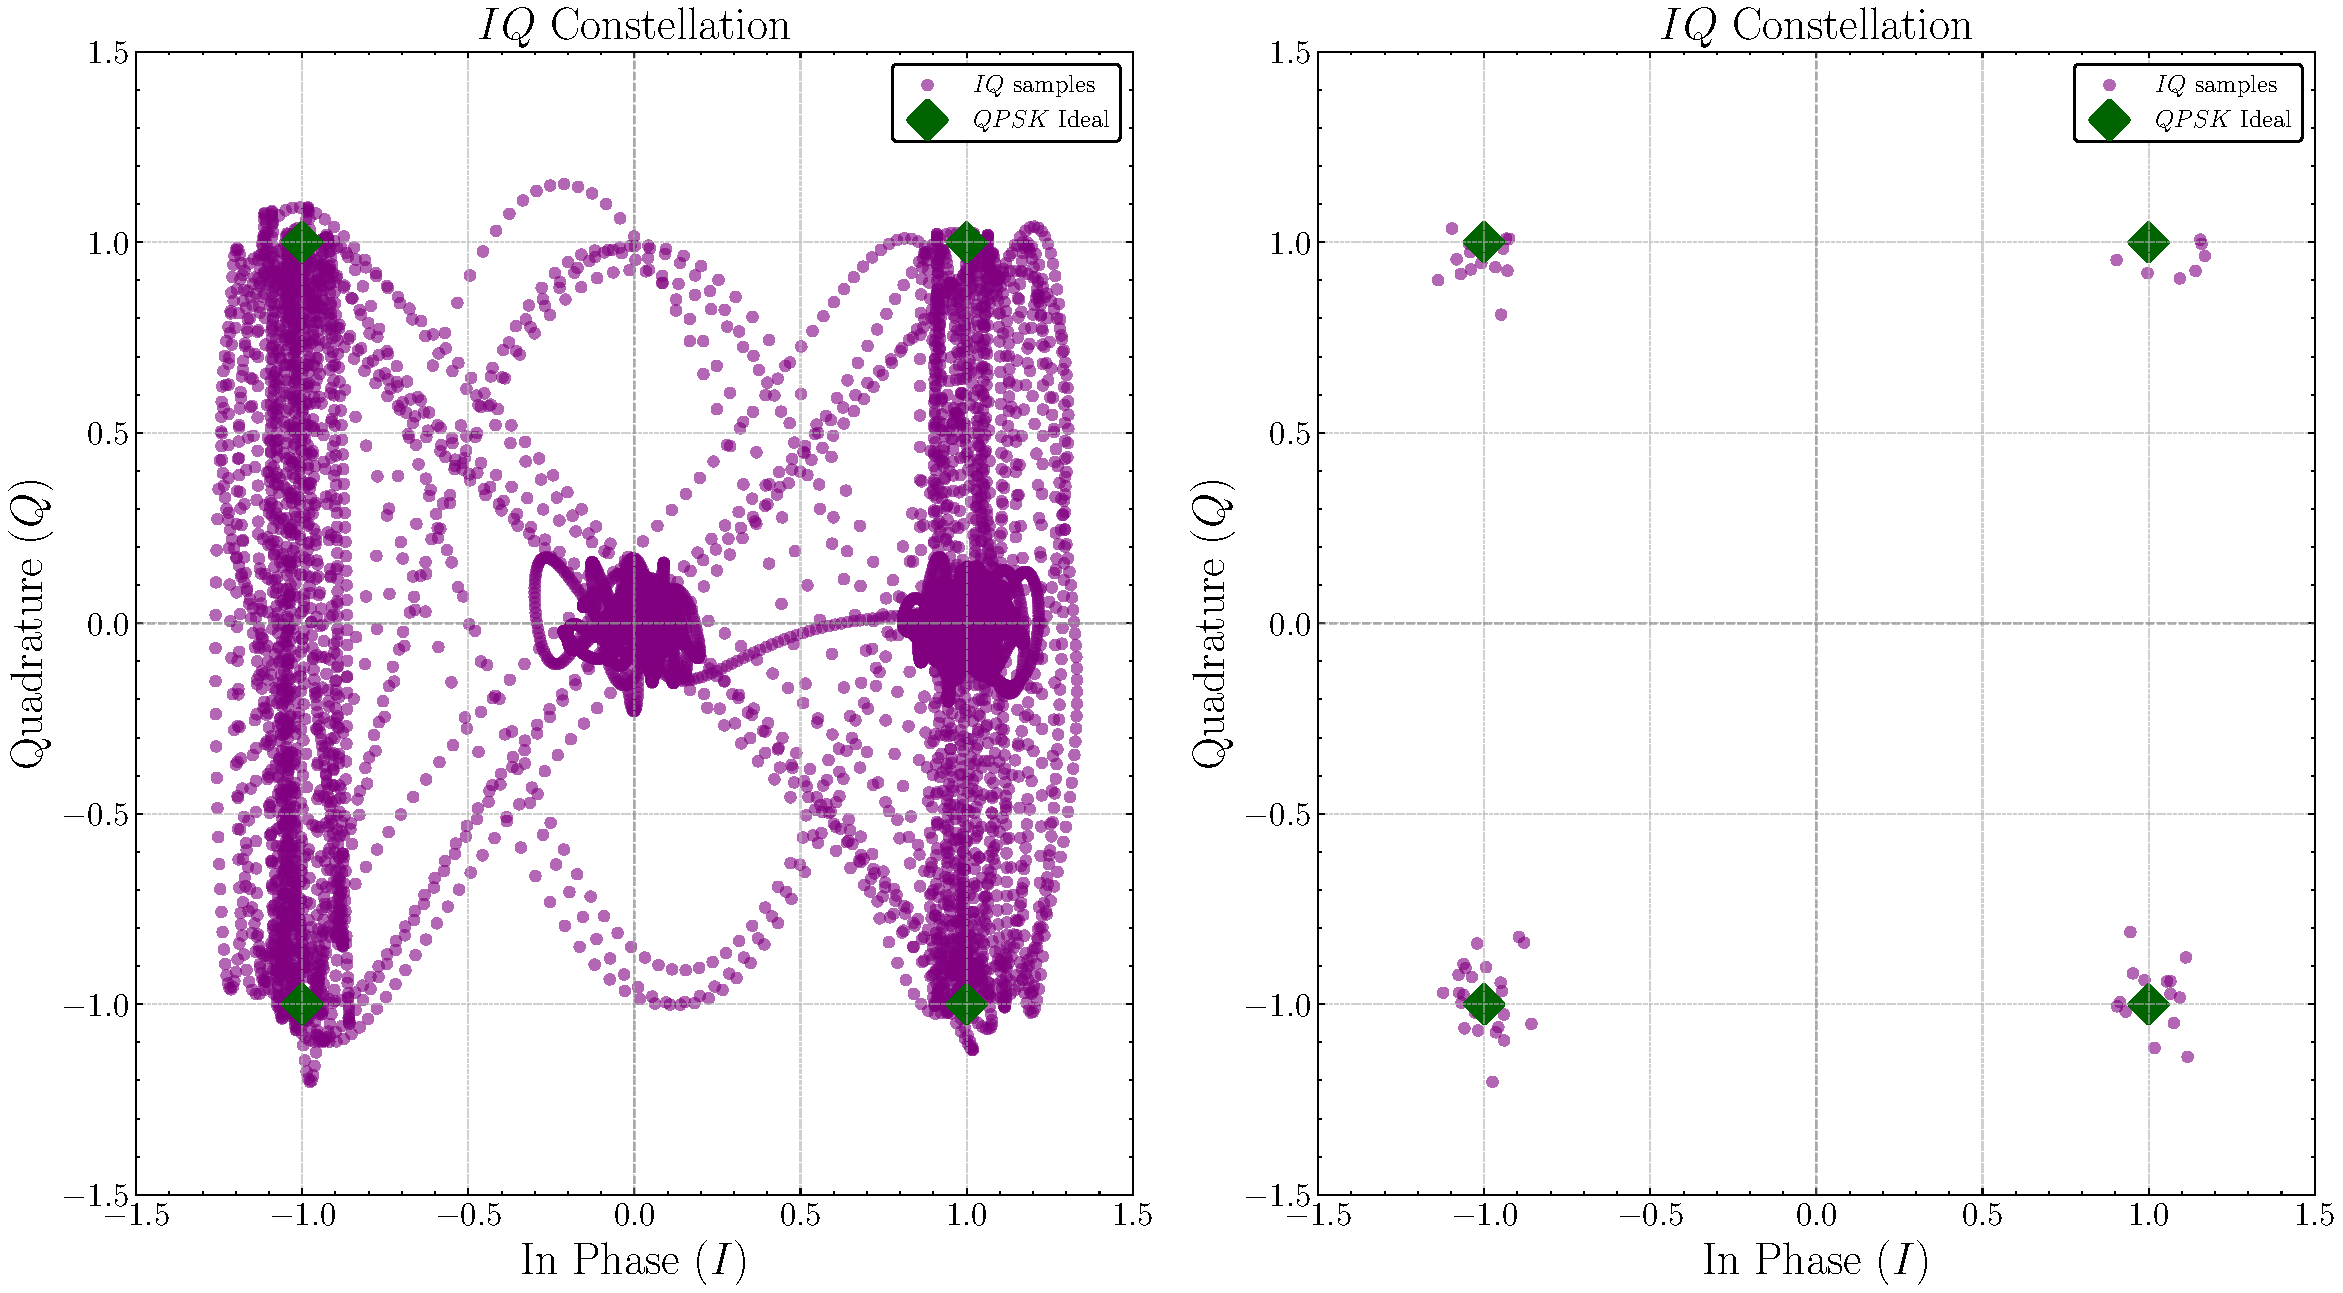
\includegraphics[width=\linewidth]{assets/cap3/receiver_sampler_const.pdf}
\end{figure}

Os vetores de amostras \gls{Inprime} e \gls{Qnprime} estão agora prontos para a recuperação do datagrama, conforme detalhado na seção \ref{sec:decodificacao_convolucional}.

\subsection{Recuperação do Datagrama}\label{sec:decodificacao_convolucional}

O último passo na cadeia de recepção é a recuperação do datagrama transmitido a partir dos vetores de amostras \gls{Inprime} e \gls{Qnprime}. O primeiro passo é o descodificador de linha, onde os vetores de amostras são convertidos de volta para bits, utilizando a técnica inversa da codificação de linha aplicada na transmissão, conforme detalhado na seção \ref{sec:line_coding}, resultando nos vetores de bits \gls{Xnprime} e \gls{Ynprime}, que precisam ser desembaralhados, conforme ilustrado na \autoref{fig:receiver_unscrambler}.

\begin{figure}[H]
	\centering
	\caption{Desembaralhamento dos canais $I$ e $Q$}\label{fig:receiver_unscrambler}
	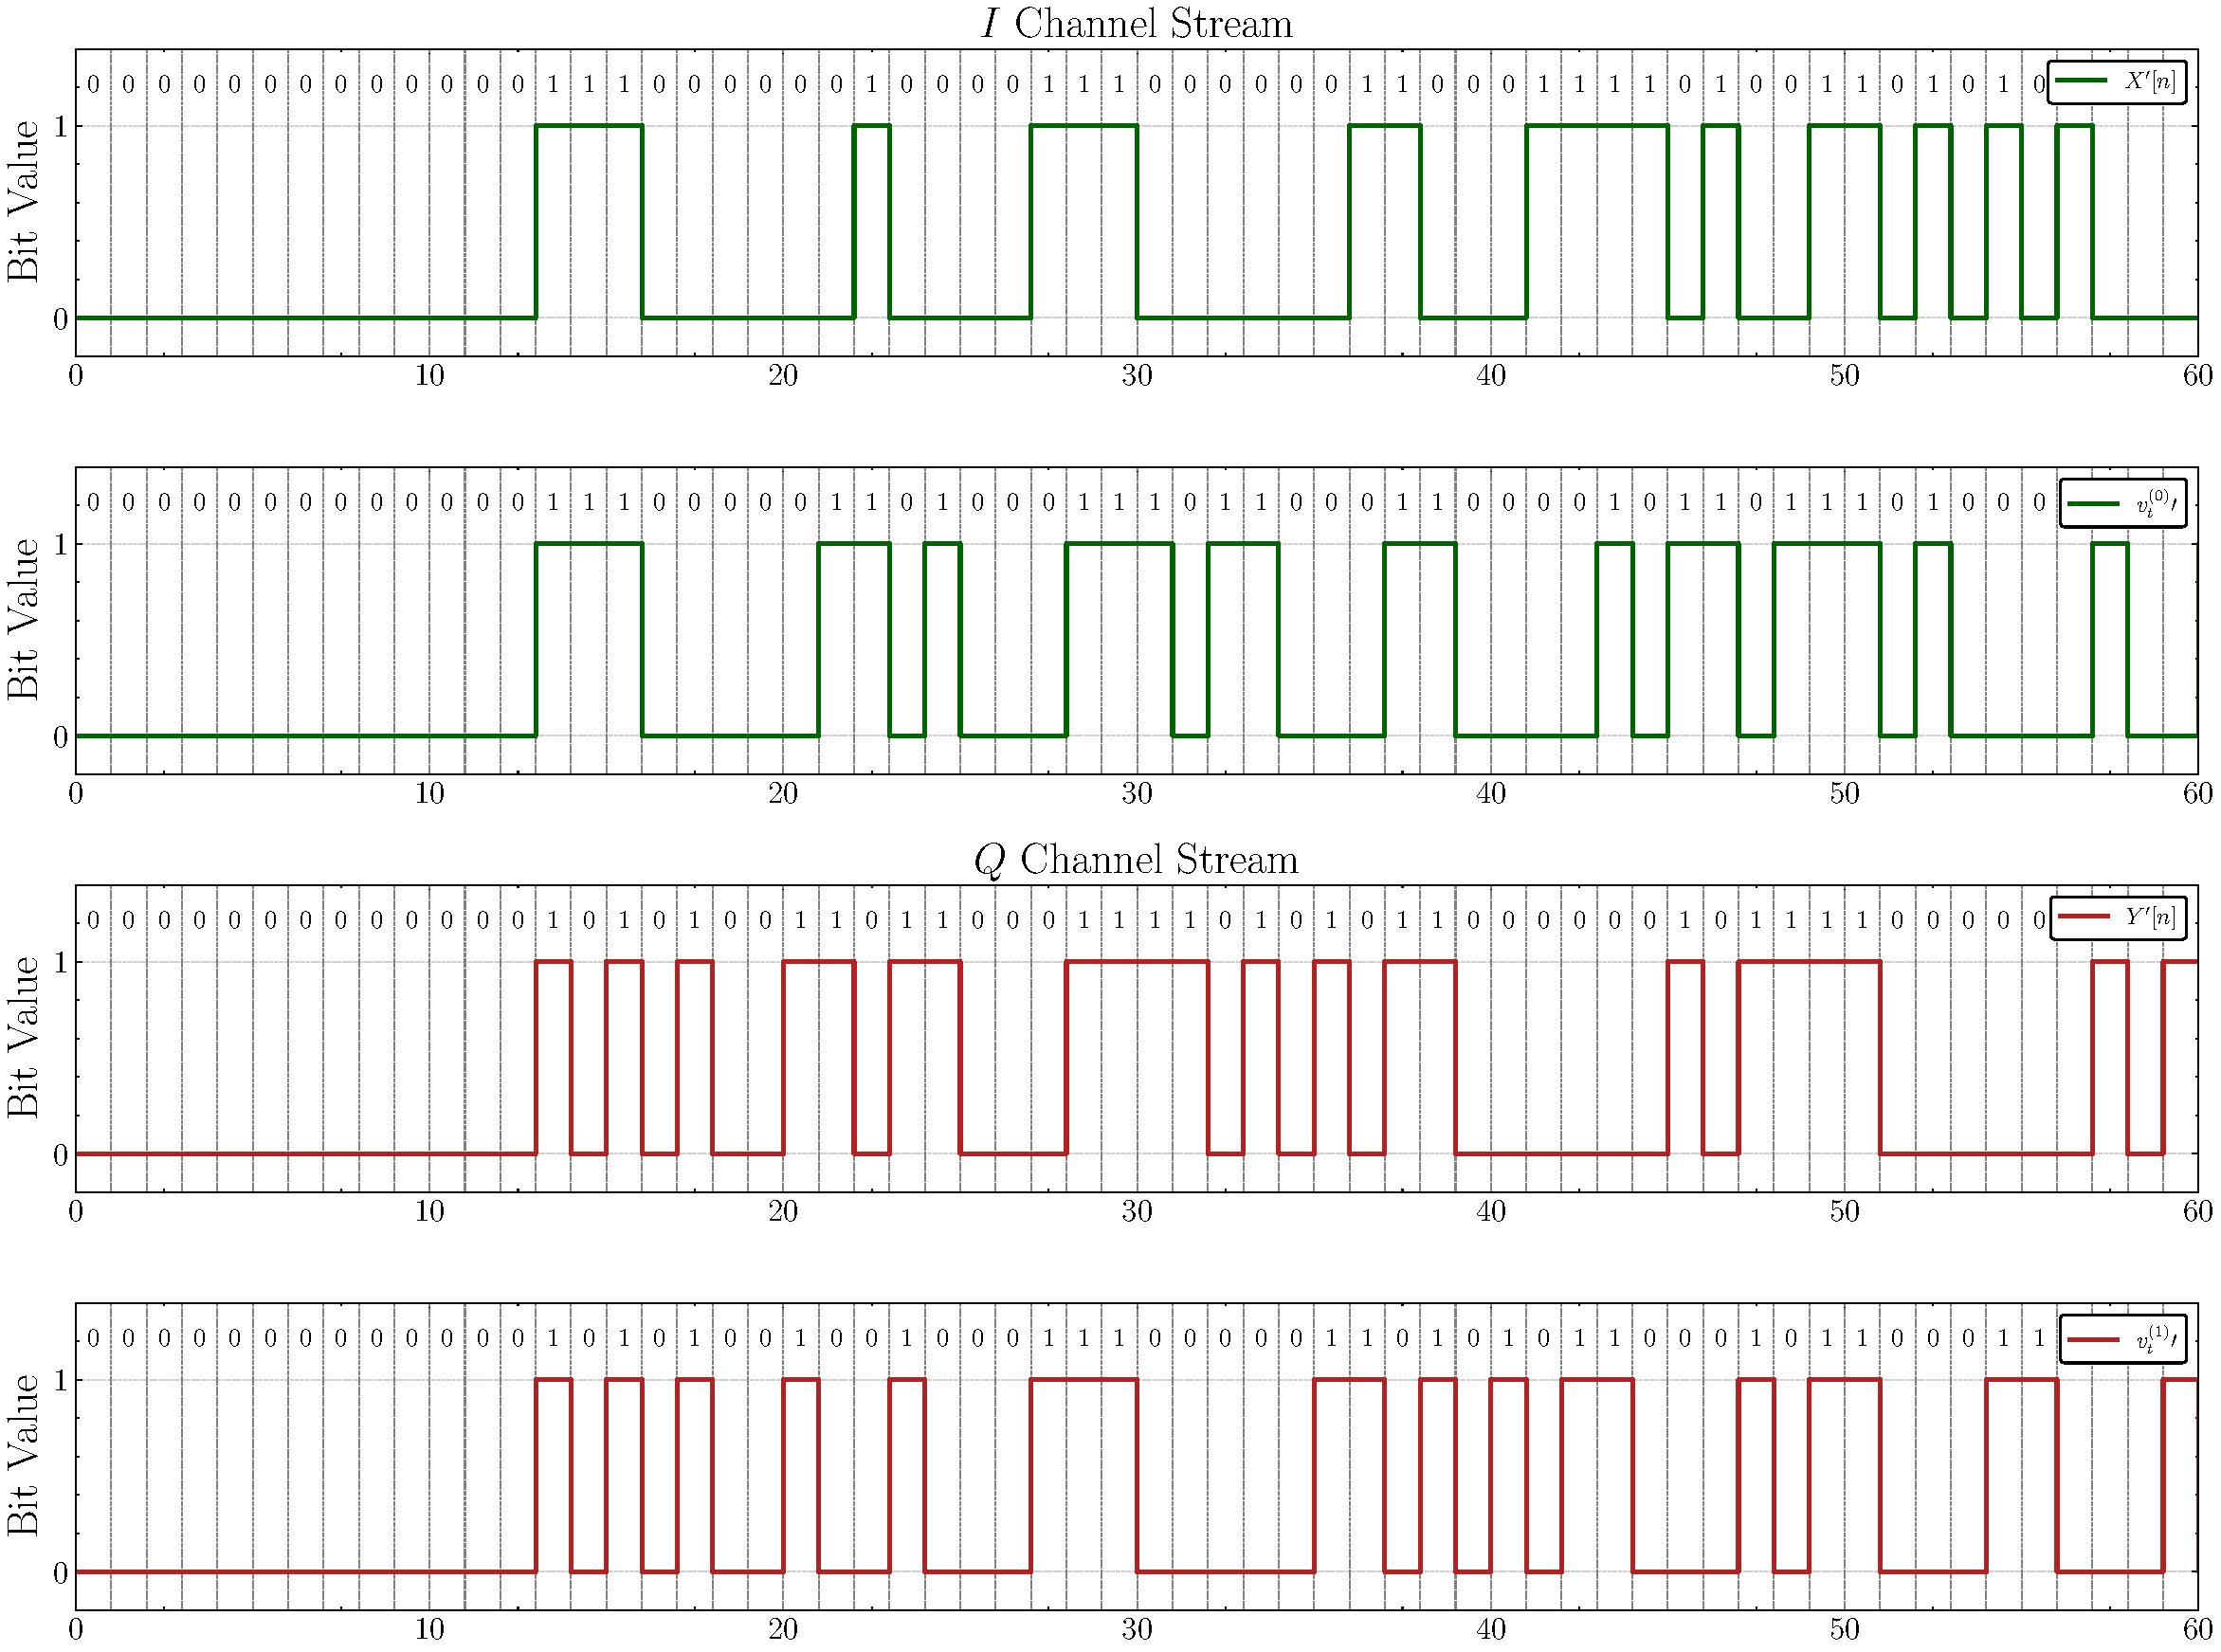
\includegraphics[width=\linewidth]{assets/cap3/receiver_descrambler_time.pdf}
\end{figure}

Os vetores de bits \gls{Xnprime} e \gls{Ynprime} desembaralhados, são então decodificados utilizando o decodificador Viterbi, conforme detalhado na seção \ref{sec:conv_coding}, resultando no vetor de bits \gls{utprime}, que representa o datagrama recuperado. O processo de decodificação convolucional é ilustrado na \autoref{fig:receiver_conv}.

\begin{figure}[H]
	\centering
	\caption{Decodificação convolucional dos canais $I$ e $Q$}\label{fig:receiver_conv}
	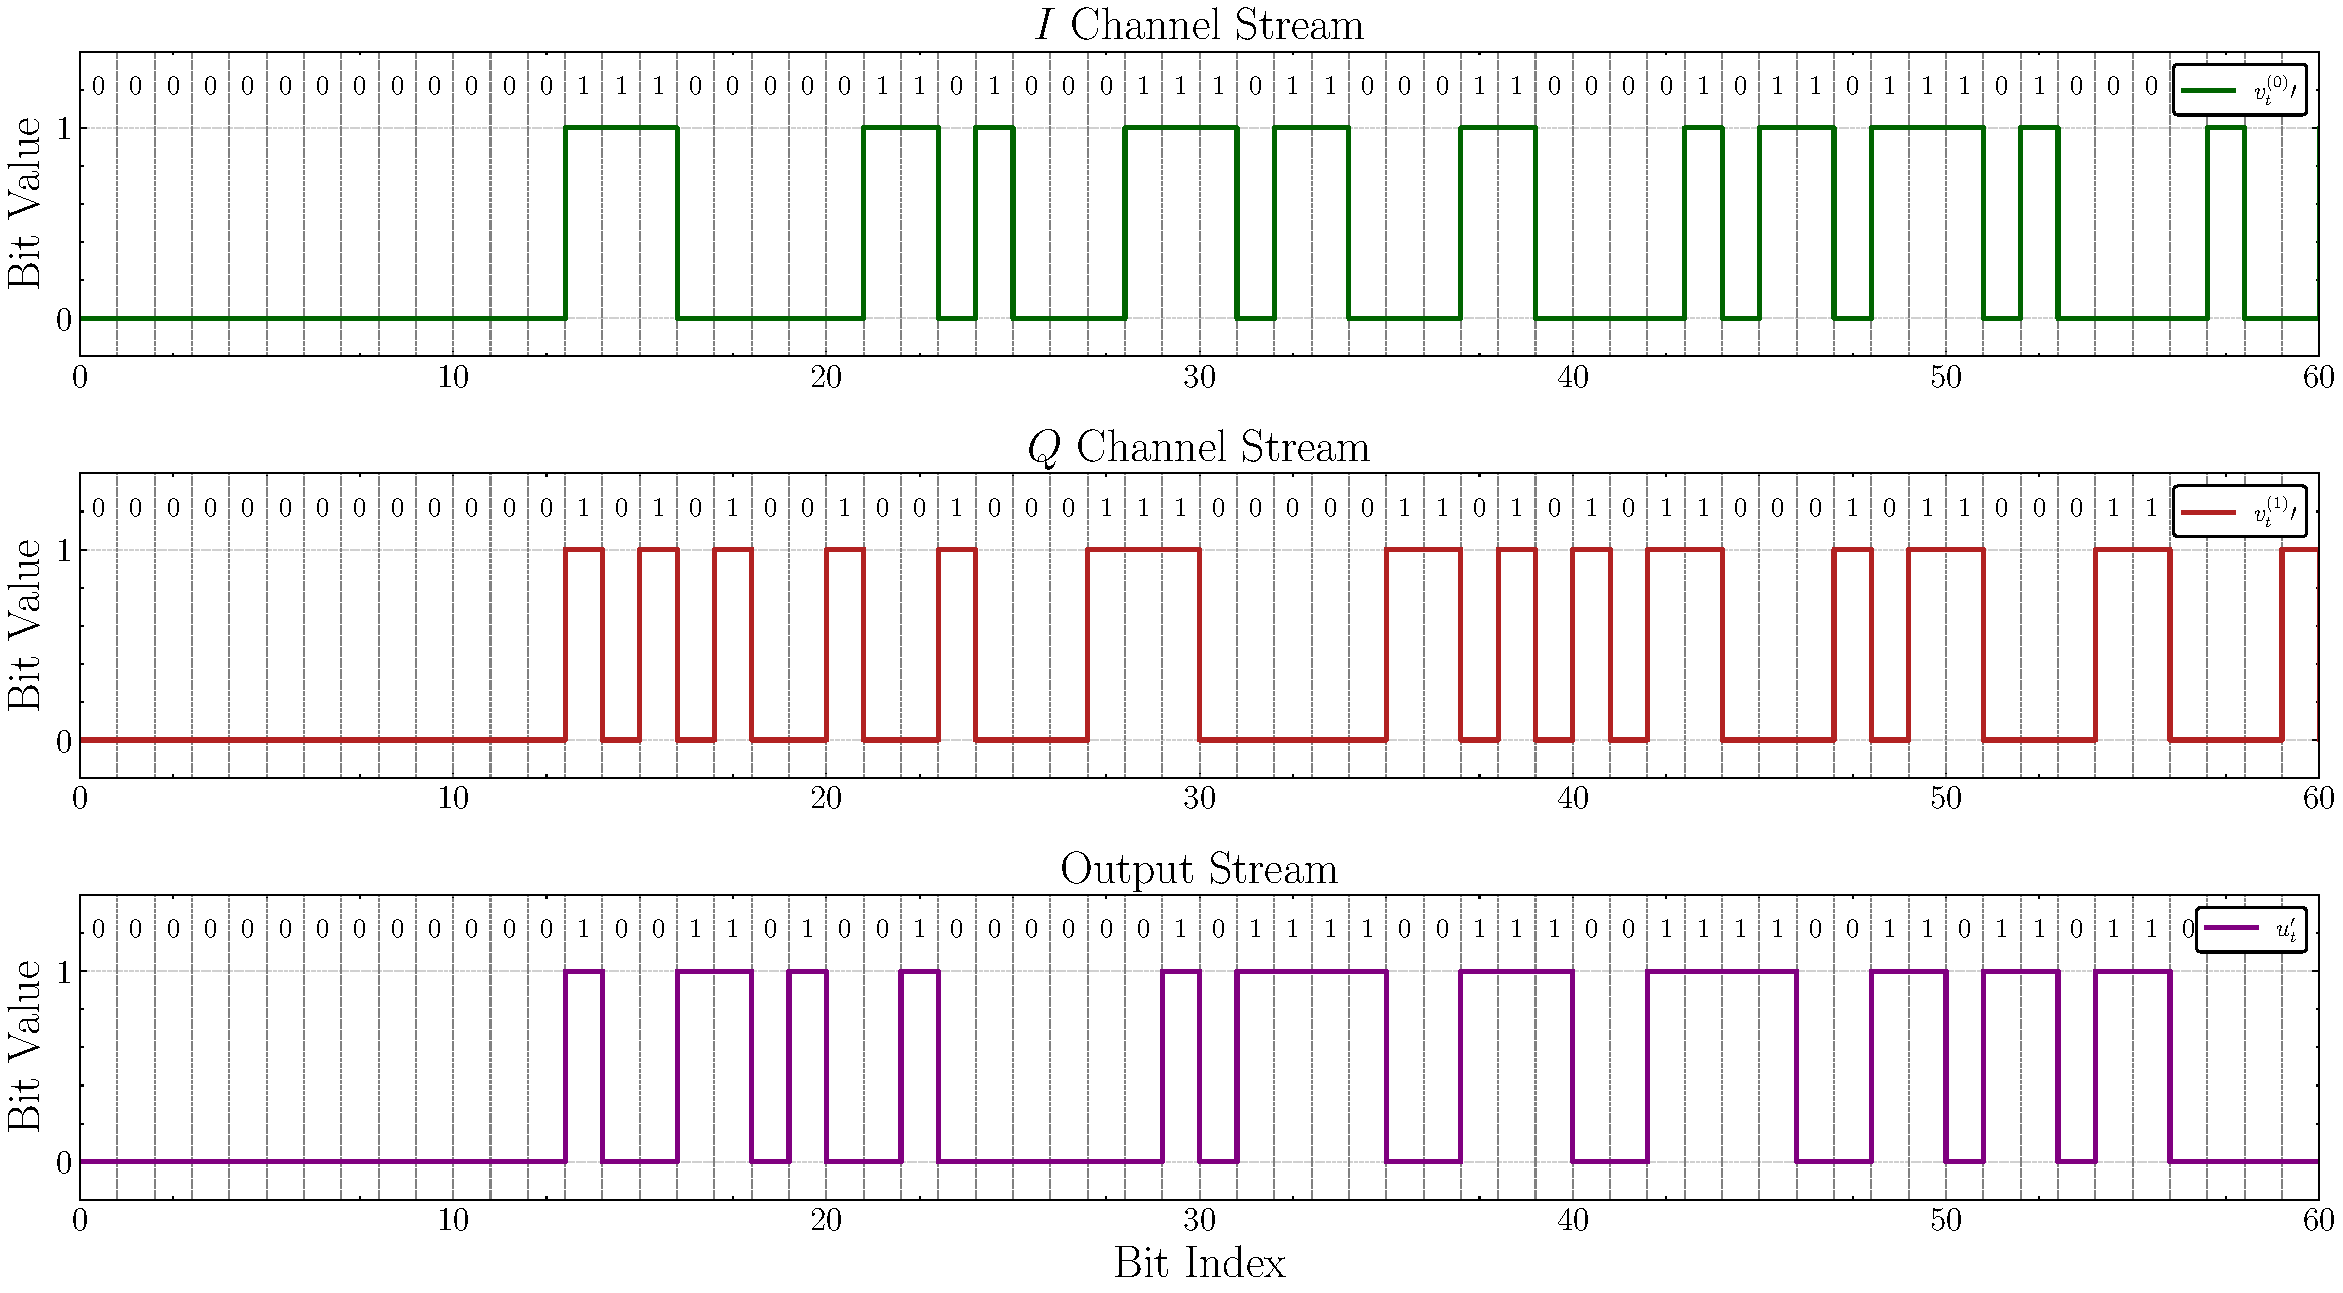
\includegraphics[width=\linewidth]{assets/cap3/receiver_conv_time.pdf}
\end{figure}

Finalmente, o vetor de bits \gls{utprime} é processado para extrair o datagrama, verificando a integridade dos dados através do campo de verificação \gls{CRC}, e então extraindo os campos de interesse, como o número de identificação da PCD \gls{pcdid} e o payload. O processo de recuperação do datagrama é apresentado no código de exemplo \ref{cod:reception}.

\lstinputlisting[language=python,caption={Parse do datagrama de $s'(t)$},label=cod:reception]{codigo/receiver.py}
